%-*-LaTeX-*-
\documentclass[11pt]{report}
%%%%%%%%%%%%%%%%%%%%%%%%%%%%%%%%%%%%%%%%
% Use the approved methods for setting lengths
%\oddsidemargin  0.0in
%\evensidemargin 0.0in
%\textwidth      6.5in
%\textheight     9.0in
\setlength{\oddsidemargin}{0.0in}
\setlength{\evensidemargin}{0.0in}
\setlength{\textwidth}{6.5in}
\setlength{\textheight}{8.7in}
% Based on document style, and taller text body height, set
% weird LaTex margin/header (box heights).  This fixes
% the disappearing page numbers (which never disappeared; they
% just got printed beyond the borders of the physical paper)
\setlength{\voffset}{0pt}
\setlength{\topmargin}{0pt}
\setlength{\headheight}{10pt}
\setlength{\headsep}{25pt}
%%%%%%%%%%%%%%%%%%%%%%%%%%%%%%%%%%%%%%%%
%\usepackage{html}
\usepackage{makeidx}
%\usepackage{times}
\usepackage{hyperref}
\usepackage{verbatim}
\usepackage{graphicx}
%\usepackage{eufrak}
\usepackage{amsmath}

\makeindex

\tolerance=600

\newcommand{\Fb}{{\bf F}}
\newcommand{\Lb}{{\bf L}}
\newcommand{\gb}{{\bf g}}
\newcommand{\nb}{{\bf n}}
\newcommand{\ub}{{\bf u}}
\newcommand{\xb}{{\bf x}}
\newcommand{\p}{\partial}
\renewcommand{\div}{{\rm div}}
\renewcommand{\arraystretch}{1.3}

\markboth{}{N. A. PETERSSON AND B. SJOGREEN; USER'S GUIDE TO SW4, v-1.0
(DRAFT)}

\begin{document}

\title{\LARGE User's guide to SW4 version 1.0 (DRAFT)} 

\author{ N. Anders Petersson$^1$ \and Bj\"orn Sj\"ogreen\thanks{Center for Applied Scientific
     Computing, Lawrence Livermore National Laboratory, PO Box 808, Livermore CA 94551. This is
     contribution LLNL-SM-XXXYYY.}}
\date{\today} 
\maketitle

%\thispagestyle{plain}

%\pagebreak
\paragraph {Disclaimer} 
This document was prepared as an account of work sponsored by an agency of the United States
government. Neither the United States government nor Lawrence Livermore National Security, LLC, nor
any of their employees makes any warranty, expressed or implied, or assumes any legal liability or
responsibility for the accuracy, completeness, or usefulness of any information, apparatus, product,
or process disclosed, or represents that its use would not infringe privately owned
rights. Reference herein to any specific commercial product, process, or service by trade name,
trademark, manufacturer, or otherwise does not necessarily constitute or imply its endorsement,
recommendation, or favoring by the United States government or Lawrence Livermore National Security,
LLC. The views and opinions of authors expressed herein do not necessarily state or reflect those of
the United States government or Lawrence Livermore National Security, LLC, and shall not be used for
advertising or product endorsement purposes. 

\paragraph{Auspices Statement}
This work performed under the auspices of the U.S. Department of Energy by Lawrence Livermore
National Laboratory under contract DE-AC52-07NA27344.
%\pagebreak
\tableofcontents


\chapter{Introduction}


\emph{SW4} is a program for simulating seismic wave propagation on parallel computers. It shares
many features with our previous seismic wave propagation code~\emph{WPP}~\cite{WPP2}. Both
\emph{WPP} and \emph{SW4} solve the seismic wave equations in second order formulation using a
node-based finite difference approach. The underlying numerical method satisfies the principle of
summation by parts, which guarentees energy stability of the numerical solution. The major
difference between \emph{WPP} and \emph{SW4} is that the latter implements a fourth order accurate spatial
discretization, complemented by a fourth order explicit time integrator~\cite{SjoPet-12}. \emph{SW4}
is therefore significantly more efficient than the second order accurate \emph{WPP} code. Compared
to a second order accurate method, the advantages of a fourth order method are more pronounced when
the solution needs to be more accurate, because the error diminishes faster as the grid size is
reduced. A fourth order method is also more efficient when the solution needs to remain accurate for
longer times, because the phase error grows as $t^{1/p}$ in a $p$th order accurate numerical
method~\cite{Gustafsson-Kreiss-Oliger}. The fourth order method is also significantly more accurate
for calculating surface waves, in particular when the ratio between the compressional and shear wave
speeds is large, i.e.~$C_p/C_s\gg 1$, see~\cite{KrePet-12}.

%% WHERE TO PUT THIS?  We have compared \emph{SW4} and \emph{WPP} on problems where the exact solution
%% is known. Compared to \emph{WPP}, \emph{SW4} gives similar accuarcy with significantly fewer grid
%% points per wave length. This means that waves with the same frequency can be resolved on a grid that
%% is coarser both in space and time. For materials with $C_p/C_s\approx 2$ and an accuracy of about 10
%% percent, the \emph{SW4} code calculates the solution about eight times faster than \emph{WPP}, using
%% about one eighth of the memory. When both codes use the same grid size, \emph{SW4} can capture waves
%% with approximately twice as high frequency.

\emph{SW4} implements substantial capabilities for 3-D seismic modeling, with a free surface
condition on the top boundary, absorbing super-grid conditions on the far-field
boundaries~\cite{PetSjo-13}, and an arbitrary number of point force and/or point moment tensor
source terms. Each source time function can have one of many predefined analytical time dependencies,
or interpolate a user defined discrete time series. \emph{SW4} supports a fully 3-D heterogeneous
material model that can be specified in several formats. It uses a curvilinear mesh near the free
surface to honor the free surface boundary condition on a realistic topography. The curvilinear mesh
is automatically generated from the description of the topography. Below the curvilinear grid, the
seismic wave equations are discretized on a Cartesian mesh, which leads to a more computationally
efficient algorithm.

\emph{SW4} solves the seismic wave equations in Cartesian coordinates. It is therefore appropriate
for regional simulations, where the curvature of the earth can be neglected. Locations can be
specified directly in Cartesian coordinates, or through geographic (latitude, longitude)
coordinates. \emph{SW4} can be built to use the Proj.4 library~\cite{Proj4} for calculating the
mapping between geographic and Cartesian coordinates, or use an approximate spheroidal
mapping. \emph{SW4} can output synthetic seismograms in an ASCII text format, or in the \emph{SAC}
format~\cite{Goldstein-et-al}. It can also present simulation information as
\emph{GMT}~\cite{WesselSmithGMT} scripts, which can be used to create annotated maps. Furthermore,
\emph{SW4} can output the solution as well as the material model along 2-D grid planes.

%In version 2.1 of \emph{SW4}, Cartesian local mesh refinement can be used to make the computational
%mesh finer near the free surface, where more resolution often is needed to resolve short wave
%lenghts in the solution, for example in sedimentary basins. The mesh refinement is performed in the
%vertical direction and each Cartesian grid is constructed from user specified refinement levels. In
%this approach, the grid size in all three spatial directions is doubled across each mesh refinement
%interface, leading to substantial savings in memory and computational effort. The energy conserving
%mesh refinement coupling method described in~\cite{PetSjo-10} is used to handle the
%hanging nodes along the refinement interface.

Visco-elastic behavior can be important when modeling the dissipative nature of realistic materials,
especially for higher frequencies. \emph{SW4} uses the rheological model of standard linear solid
(SLS) elements, coupled in parallel. The coefficients in each SLS are determined such that the
resulting quality factors $Q_p$ and $Q_s$, for the attenuation of P- and S-waves, become
approximately constant as function of frequency. These quality factors can vary from grid point to
grid point over the computational domain and are read in the same way as the elastic properties of
the material model. The numerical method for solving the visco-elastic wave equation is
based on the technique described in~\cite{PetSjo-10b}.

While most of the \emph{SW4} code is written in C++, almost all numerical computations are
implemented in Fortan-77. \emph{SW4} uses a distributed memory programming model, implemented with
the C-bindings of the MPI library. Compatible versions of the C++ and Fortran-77 compilers as well
as the MPI library must therefore be available to build the code. We have built and tested
\emph{SW4} on a variety of machines, ranging from single processor laptops to large super-computers
with ${\cal O}(10,000)$ cores.

With the exception of some minor details, the syntax of the \emph{SW4} command file is the same as
in \emph{WPP}. Most of the input and output files also use the same formats, but we have taken the
opportunity to improve the image file format (see Chapter~\ref{chap:formats} for details). With the
exception of mesh refinement, version 1.0 of \emph{SW4} supports most of the functionality of
\emph{WPP} (version 2.2). We hope to add the remaining features in the future.

The {\tt examples} subdirectory of the \emph{SW4} source distribution contains several examples and
validation tests that are used in this document. Many Matlab/octave scripts are are provided in the
{\tt tools} directory.
%and described in Chapter~\ref{chap:scripts}.

\section*{Acknowledgments} 
The \emph{SW4} code was developed under financial support from Lawrence Livermore National
Laboratory. The underlying numerical method was developed under financial support from
the Office of Science at the U.S.~Department of Energy.


%%%%%%%%%%%%%%%%%%%%%%%%%%%%%%%%%%%%%%%%%%%%%%%%
\chapter{Getting started}
\index{srun}\index{parallel execution}
%%%%%%%%%%%%%%%%%%%%%%%%%%%%%%%%%%%%%%%%%%%%%%%%

\section{Running \emph{SW4}}
This section assumes that \emph{SW4} has already been installed on your system. For instructions on
how to build \emph{SW4} from the source code distribution, see Appendix~\ref{cha:installing-sw4}.

\emph{SW4} can be executed from the command prompt or from a script. The simulation is specified by
the input file, and the name of the input file is given on the command line. The input file is an
ASCII text file that contains a number of commands specifying the properties of the simulation, such
as the dimensions of the computational domain, grid spacing, the duration of the simulation, the
material properties, the source model, as well as the desired output. To improve readability of this
document we have used the continuation character ``$\backslash$" to extend long commands to the
subsequent line. There is however no support for continuation characters in \emph{SW4}, so each
command must be given on one (sometimes long) line in the input file.

Since \emph{SW4} is a parallel code, it is required to be run under a parallel execution environment
such as mpiexec, mpirun, openmpirun, or srun. The srun command is currently always used on the
parallel machines at Livermore computing. On other machines, it is important to start \emph{SW4}
with the correct parallel execution tool. For example, if you build \emph{SW4} with the openmpi
compilers, you should use the openmpirun environment. Also note that some systems require you to
start an \verb+mpd+ daemon before running any parallel programs. Chances are high that somebody else
has already figured out how to run parallel programs on your system, and we recommend talking to
your local system administrator, or somebody else with experience running MPI programs on your system.

Throughout this document we use the convention that input files have the file suffix {\tt
  .in}. However, \emph{SW4} will attempt to read any input file, regardless of its extension.

If your system is setup for using \verb+mpiexec+, the command
\begin{verbatim}
	shell> mpiexec -np 2 sw4 test.in
\end{verbatim}
runs \emph{SW4} on 2 processes, and tells it to read input from a file named {\tt test.in}.  If you
are using \verb+mpirun+, you would instead use the command
\begin{verbatim}
	shell> mpirun -np 2 sw4 test.in
\end{verbatim}
{\bf Remark: }
If \emph{SW4} produces strange looking outputs, for example where the same text is repeated several times (e.g. once
per processor), you are probably running \emph{SW4} under the wrong parallel execution
environment. Make sure you are running \emph{SW4} under an environment which is compatible with the
compiler that was used to build \emph{SW4}.
%

\subsection{Version information (-v)}
\index{command line options!-v version info}

Version information for the \emph{SW4} executable can be obtained through {\tt -v} flag:
\begin{verbatim}
[yorkville:~/src/sw4/src] petersson1% openmpirun -np 2 ./sw4 -v
----------------------------------------------------------------
            sw4 version 1.0

 This program comes with ABSOLUTELY NO WARRANTY; released under GPL.
 This is free software, and you are welcome to redistribute     
 it under certain conditions, see LICENSE.txt for more details  
----------------------------------------------------------------
  Compiled on: Fri Feb 22 08:31:41 PST 2013
  By user:     petersson1
  Machine:     yorkville.llnl.gov
  Compiler:    /opt/local/bin/openmpicxx
  3rd party software include directory: /Users/petersson1/include
  3rd party software library directory: /Users/petersson1/lib
-----------------------------------------------------------------
\end{verbatim}
Note that the same information is by default printed to standard out (your screen, or log file when
running in batch mode) at the beginning of every run.

\subsection{Running on the Livermore Computing parallel linux clusters}
%
The srun command is currently used to run parallel jobs on LC machines. For example, the command
\begin{verbatim}
	shell> srun -ppdebug -n 32 sw4 xxx.in
\end{verbatim}
runs \emph{SW4} on 32 processors on the debug parition using xxx.in as the input file. Note that the
pdebug partition is intended for shorter jobs. It is subject to both a CPU time limit and a limit on
the number of processors per job. Jobs requiring more computer resources must be submitted through
the batch system, currently using the msub command. Refer to the Livermore Computing web pages for
detailed information (https://computing.llnl.gov).

%\section{Warning and error messages}

%Warning and error messages are stored in separate log files...

%%%%%%%%%%%%%%%%%%%%%%%%%%%%%%%%%%%%%%%%%%%%%%%
\chapter{Governing equations, coordinate system, and units}
\index{coordinate system}\index{units}
%%%%%%%%%%%%%%%%%%%%%%%%%%%%%%%%%%%%%%%%%%%%%%%
%
\emph{SW4} simulates the motion due to a seismic event by solving the elastic (or visco-elastic) 
wave equation in second order formulation. The equations are solved in the spatial domain 
${\bf x}\in\Omega$ during the time interval $0\leq t\leq T$. By default, the motion starts from rest and is driven by
a forcing function ${\bf F}({\bf x},t)$,
\begin{alignat}{3}
\rho {\bf u}_{tt} &= \nabla\cdot{\cal T} + {\bf F}({\bf x},t),&\quad\mbox{${\bf x}$ in
  $\Omega$},\ 0\leq t\leq T,\label{eq:elastic-we}\\ 
{\bf u}({\bf x},0)&=0,\quad {\bf u}_t({\bf x},0) = 0, &\quad\mbox{${\bf x}$ in $\Omega$}.
\end{alignat}
Here, $\rho$ is the density, ${\bf u}({\bf x},t)$ is the displacement vector, and ${\cal T}$ is the
stress tensor. The computational domain $\Omega$ is a box shaped region where one side optionally
follows the shape of the topography. By default, a free surface (zero traction, or normal stress)
boundary condition is enforced along the top boundary,
\[
{\cal T} \cdot \nb = 0,\quad z=\tau(x,y),\ t\geq 0.
\]
Here $\nb$ is the unit normal of the $z=\tau(x,y)$ surface. By default, a super-grid damping layer
surrounds the computational domain on all other sides of the computational domain.

\emph{SW4} uses a right-handed Cartesian coordinate system with the z-direction pointing
downwards into the medium, see figure~\ref{fig:coordsys}. 
\begin{figure}[th]
\begin{centering}
 \includegraphics[width=0.6\linewidth]{coords.png}
  \caption{\emph{SW4} uses a right handed coordinate system with the z-axis pointing
  downwards.}
  \label{fig:coordsys}
\end{centering}
\end{figure}
\emph{SW4} employs MKS (meters-kilograms-seconds) units. All distances (e.g.,~grid dimensions,
spacing, and displacements) are in meters (m), time is in seconds (s), seismic P- and S-wave
velocities are in meters per second (m/s), densities are in kilogram per cubic meter (kg/m$^3$),
forces are in Newton (N), and seismic moment (torque) is in Newton-meters (Nm). All angles
(e.g. latitude, longitude, azimuth, strike, dip and rake) are in degrees. 
%The quality factors $Q_P$ and $Q_S$ are dimensionless.

In \emph{SW4} the computational domain is rectangular in the horizontal plane and the vertical extent
is defined by the topography surface
\[
z=\tau(x,y),
\]
which defines the shape of the free surface. \emph{SW4} can also be run with flat topography, in
which case $\tau(x,y)=0$ and the $z$-coordinate is the depth below the free surface. In the general
case, the computational domain is given by
\begin{equation}\label{eq:domain}
0\leq x\leq x_{max},\quad 0\leq y\leq y_{max},\quad \tau(x,y) \leq z \leq z_{max}.
\end{equation}

The grid command in the input file specifies the extent of the computational domain and the grid
size $h$. When topography is enabled, the grid size in the curvilinear grid equals $h$ in the
horizontal directions, but varies in the vertical direction to allow the curvilinear grid to follow
the shape of the free surface. In this case, the number of grid points in the vertical direction is
chosen such that the average of the vertical grid size approximately equals $h$.
%When mesh refinement is enabled, this is the grid size in the
%coarsest grid. 

The most obvious way of specifying the grid is by providing the number of grid points in each
direction as well as the grid size,
%
\begin{verbatim}
	grid nx=301 ny=201 nz=101 h=500.0 
\end{verbatim}
%
This command gives a grid with grid size 500 meters, which extends 150 km in $x$, 100 km in $y$ and
50 km in the $z$-direction. Alternatively, the grid can be specified by giving the spatial range in
each of the three dimensions and explicitly specifying the grid spacing. For example, the command
%
\begin{verbatim}
	grid x=30e3 y=20e3 z=10e3 h=500.0 
\end{verbatim}
%
results in a grid which spans 30,000 meters in $x$, 20,000 meters in $y$, and 10,000
meters in the $z$-direction.  The grid spacing is 500 meters, which is used to compute the
number of grid points in each direction: nx=61, ny=41, and nz=21, for a total of
52,521 grid points. Note that the number of grid points in the different directions will be
rounded to the nearest integer value according to the pseudo C-code
\begin{equation}\label{eq:nx-calculation}
nx = \mbox{(int)} (1.5 + x/h).
\end{equation}
The extent in the $x$-direction is thereafter adjusted to
\begin{equation}\label{eq:x-calculation}
x=(nx-1) h.
\end{equation}
A corresponding procedure is performed in the other coordinate directions.

The third option is to give the spatial range in each of the three dimensions and specify the number
of grid points in a particular direction:
%
\begin{verbatim}
	grid x=30000 y=20000 z=10000 nx=100
\end{verbatim}
%
In this case, the grid spacing is computed as 
\[
h = x/(nx-1)= 303.03.
\]
Note that no rounding needs to take place in this case, since $h$ is a floating point number. Given this
value of $h$, ny and nz are computed using formulas corresponding to
(\ref{eq:nx-calculation}) giving ny=34 and nz=67, for a total of 227,800 grid points. Again,
the extents in the $y$ and $z$-directions are adjusted corresponding to (\ref{eq:x-calculation}). The syntax
for the grid command is given in Section~\ref{keyword:grid}.

The simulation always starts at $t=0$ and runs until $t=T$, where the user must specify $T$ with the
{\tt time} command. For example,
\begin{verbatim}
time t=1.6
\end{verbatim}
sets $T=1.6$ seconds. Alternatively, the simulation time interval can be specified as 
a number of time steps, as in the example
\begin{verbatim}
time steps=1200
\end{verbatim}
Here the number of time steps is set to 1200. The end time will in this case be $T=1200\Delta t$,
where the time step $\Delta t$ is determined automatically by \emph{SW4} to satisfy the CFL time
step restriction. This calculation is based on the ratio between the grid size and the largest
characteristic wave speed, which depends on both the compressional and shear wave speeds. 

The simulation start time can be related to a universal time coordinate (UTC). The option {\tt
  utcstart} sets the UTC that corresponds to simulation time $t=0$, for example,
\begin{verbatim}
time t=1.6 utcstart=01/31/2012:17:34:12.233
\end{verbatim}
The format of the UTC is ``month/day/year:hour:minute:second.millisecond''. When the UTC time
is set, it is saved in the header of all time series files (see the {\tt rec} command). Note that
the UTC can be very useful for aligning simulated and observed time series.
%is also used the inverse problem with \emph{SW4opt}.

\section{Geographical coordinates and projections}
\index{geographical coordinates}
\emph{SW4} supports geographical coordinates as an alternative way of specifying spatial
locations. The geographic location of the origin of the Cartesian coordinte system (lat$_0$,
lon$_0$), see Figure~\ref{fig:geocoord}, is specified in the grid command. 
\begin{figure}
\begin{centering}
  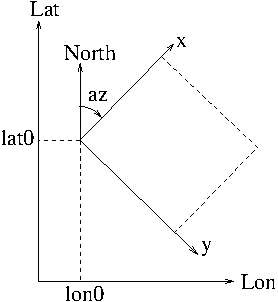
\includegraphics[width=0.5\linewidth]{latlon.png}
%  \includegraphics{LatLonAz.ps}
  \caption{Geographical coordinates in \emph{SW4}.}
  \label{fig:geocoord}
\end{centering}
\end{figure}
If no location is given, the default location is lat$_0$ = 37 degrees (North), lon$_0$ = -118
degrees (West), and the azimuthal angle of the $x$-axis is 135 degrees from North. The vertical
coordinate increases downwards. For the case of general topography, $z=0$ corresponds to mean sea
level. When the topography is flat (no {\tt topography} command in the input file), $z=0$
corresponds to the free surface.

\subsection{Spheroidal mapping}
By default, the latitude (lat) and longitude (lon) are calculated using a spheroidal mapping,
\begin{alignat}{2}
\mbox{lat} &= \mbox{lat$_0$} + \frac{x\cos(\alpha) - y\sin(\alpha)}{M},\quad \alpha =
\mbox{az}\frac{\pi}{180}, \label{eq:lat}\\
\mbox{lon} &= \mbox{lon$_0$} + \frac{x\sin(\alpha ) + y\cos(\alpha)}{M\cos(\phi \pi/180)}.\label{eq:lon}
\end{alignat}
In this formula, lat, lon, az, lat$_0$, and lon$_0$ are all in degrees, and $M = 111,319.5$
meters\footnote{Note that $M/60 = 1,855.325$ meters corresponds to one minute of arc of
  longitude along the Equator on the WGS84 ellipsoid. This distance is also known as a geographical
  mile and is approximately equal to a Nautical mile (1,852 meters).}.  You can change the location
and orientation of the grid by specifying the latitude and longitude of the grid origin, as well as
the azimuthal angle between North and the $x$-axis. For example:
\begin{verbatim}
grid h=500 x=30000 y=20000 z=10000 lat=39 lon=-117 az=150
\end{verbatim}
sets the origin of the grid to latitude 39 degrees (North), longitude -117 degrees
(West), and azimuthal angle 150 degrees.

The default projection is spheriodal as described by equations \eqref{eq:lat}-\eqref{eq:lon}. You
can change the parameter $M$ with the {\bf mlat} keyword in the {\bf grid} command. By using the
{\bf mlon} keyword, you can also modify the projection by replacing $M\cos(\phi\pi/180)$ in
\eqref{eq:lon} by the constant value $M_{lon}$. Using the {\bf mlon} keyword is only recommended if
the computational domain is small and accurate values of both {\bf mlon} and {\bf mlat} are
available.

\subsection{The Proj.4 library}
More accurate projections are available through the Proj4 library (if
\emph{SW4} was built with Proj4 support). These projections are enabled by using the {\bf proj}
and/or {\bf ellps} keywords in the {\bf grid} command. For example,
\begin{verbatim}
grid h=300 x=40e3 y=43e3 z=40e3 lat=45.01 lon=5.52 az=0 proj=utm ellps=WGS84
\end{verbatim}
sets the origin of the grid to latitude 45.01 degrees (North), longitude 5.52 degrees (East), and
azimuthal angle 0. Here we use the UTM projection based on the WGS84 ellipse. Note that the strings
``proj=utm'' and ``ellps=WGS84'' are passed directly to the Proj4 library to initialize the
projection. Many other options are available. See the Proj4 documentation~\cite{Proj4} for further
details.

\section{Super-grid damping layers}

\emph{SW4} implements a super-grid modeling technique to reduce artificial reflections from the
far-field boundaries~\cite{AppCol-09, PetSjo-13}. In this method, a coordinate mapping (stretching
function) is used to map the computational domain onto a much larger physical domain, so that it
takes a very long time for the waves to arrive at the outer boundary. The streching is combined with
a high order artificial dissipation operator that added in the super-grid layers. It damps out waves
that become poorly resolved on the grid, because of the stretching. Note that the dissipative term
is only added in the layers, and should not affect the accuracy in the interior of the domain.

The coordinate stretching compresses the solution inside the layers. This corresponds to a slowing
down of all traveling waves in the direction normal to each far-field boundary. As a result, the
isotropic elastic wave equation becomes anisotropic in the super-grid layers. It is possible to
prove by energy estimates that the super-grid modeling leads to a stable numerical method with
decreasing energy. This estimate is valid for heterogeneous material properties and free surface
boundary conditions on one or more sides of the domain. See the paper by Petersson and
Sjogreen~\cite{PetSjo-13} for more details.

Super-grid layers are included on all sides of the computational domain, except along the
free surface, see Figure~\ref{fig:layout}.
\begin{figure}[th]
\begin{center}
%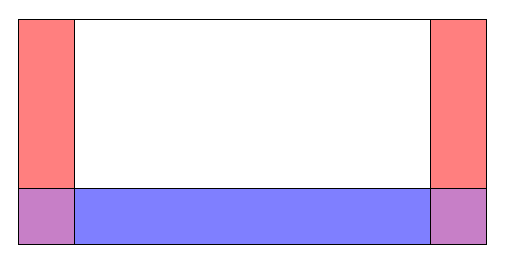
\includegraphics[width=0.65\linewidth]{layout.eps}
\includegraphics[width=0.65\linewidth]{layout.png}
\caption{\em A vertical cross-section through the computational domain with a free surface boundary
  along the top edge. The original seismic wave equation is solved the white region. The wave speed
  is reduced in the normal direction of the surrounding super-grid layers, where also a high order
  damping term is added.}\label{fig:layout}
\end{center}
\end{figure}
The default thickness of the layers (currently) equals 30 grid sizes, but the thickness of the
super-grid layers can be changed with the {\tt supergrid} command, see
Section~\ref{sec:supergrid}. Note that long waves are harder to suppress than short waves. This is
one reason why a thicker super-grid layer leads to smaller artificial reflections.

For practical reasons, the super-grid layers are part of the computational domain as specified by
the grid command. If, for example, each super-grid layer is 30 grid points wide, the solution
should be considered artificial in the first and last 30 points in each horizontal direction, and
the bottom 30 points in the vertical direction. Note that the numerical solution within the layers
do {\em not} approximate the solution of the seismic wave equation. For this reason, it is important
to make the computational domain sufficiently large. If the super grid layers are 30 grid points
wide, the computational grid must be at least 60 grid points wide in the $x$ and $y$-directions, and
30 points wide in the Cartesian part of the $z$-direction. Additional grid points must be added in
the interior of the computational domain for the actual seismic modeling. Note that sources and
receivers should only be placed in the interior of the computational domain, i.e., the white region
of Figure~\ref{fig:layout}.

%%%%%%%%%%%%%%%%%%%%%%%%%%%%%%%%%%%%%%%%%%%%%%%%
\chapter{Sources, time-functions, and grid size}
%%%%%%%%%%%%%%%%%%%%%%%%%%%%%%%%%%%%%%%%%%%%%%%%

%The source time function can be selected from a set of predefined functions, or by spline
%interpolation of a user defined discrete time-series. Each point force or point moment tensor source
%can have a different time function. 

\section{Point force and moment tensor sources in \emph{SW4}}\label{sec:time-functions}
The forcing term ${\bf F}$ in equation \eqref{eq:elastic-we} consists of a sum of point forces and
point moment tensor source terms. For a point forcing we have
\[
{\bf F}({\bf x},t) = g(t,t_0,\omega) F_0 \left(\begin{array}{c}
  F_x\\ F_y\\ F_z\end{array}\right) \delta ({\bf x} - {\bf x_0}),
\]
where ${\bf x}_0=(x_0,y_0,z_0)$ is the location of the point force in space, and $g(t,t_0,\omega)$
is the time function, with offset time $t_0$ and frequency parameter $\omega$. The source time
function can be selected from a set of predefined functions, or by spline interpolation of a user
defined discrete time-series. The $(F_x,F_y,F_z)^T$ vector holds the Cartesian components of the force
vector, which is scaled by the force amplitude $F_0$. 

For a moment tensor source we have
\[
{\bf F}({\bf x},t) = g(t,t_0,\omega)\, {\cal  M} \cdot \nabla \delta ({\bf x} - {\bf
  x_0}), \quad 
{\cal M} = \left(\begin{array}{ccc}
M_{xx} & M_{xy} & M_{xz}\\
M_{xy} & M_{yy} & M_{yz}\\
M_{xz} & M_{yz} & M_{zz}
\end{array}
\right).
\]
The seismic moment of a moment tensor source is defined by 
\[
M_0 = \sqrt{{\cal M}:{\cal M}} = \left[ (M_{xx}^2 + M_{yy}^2 + M_{zz}^2 ) + 2 (M_{xy}^2 + M_{xz}^2 + M_{yz}^2) \right]^{1/2}.
\]
Note that the moment tensor is always symmetric. A moment source term can alternatively be specified
by using $M_0$ and the dip, strike, and rake angles, as defined by Aki and
Richards~\cite{Aki-Richards-02}. The syntax is described in Section~\ref{keyword:source}.

The total seismic moment $\sum M_0$ [Nm] is related to the moment magnitude by the formula
\[
M_W = \frac{2}{3}\left[\log_{10}\left(\sum M_0\right) - 9.1\right].
\]
After parsing all source commands in an input file, \emph{SW4} outputs the moment magnitude using
this formula. This information is given right before the time-stepping is started and looks like this:
\begin{verbatim}
-----------------------------------------------------------------------
  Total seismic moment (M0): 1.7162e+17 Nm 
  Moment magnitude     (Mw): 5.42305
  Number of sources 542
-----------------------------------------------------------------------
\end{verbatim}
Note that the calculation of the total seismic moment and magnitude only take the moment tensor sources into
account, i.e., ignores all point forces.

For moment tensor sources, the function $g(t)$ is called the moment history time function, while its
time derivative $g'(t)$ is known as the moment rate time function. \emph{SW4} calculates the
displacements of the motion corresponding to the moment history time function $g(t)$. Because
the material properties are independent of time, the equations solved by {\emph SW4} also govern the
velocities when the time function is replaced by $g'(t)$, i.e., the corresponding moment rate time
function. For example, if the solution calculated with the {\tt GaussianInt} time function
represents the displacements of the motion, the solution calculated with the {\tt Gaussian} time
function corresponds to the velocities of the same motion. Hence, if you are primarily interested in
calculating velocities, you can reduce the amount of post processing by using the corresponding
moment rate time function in the source term(s). 

If you are interested in comparing results from \emph{SW4} with some other code, keep in mind that
many other seismic wave propagation codes are based on the first order velocity-stress formulation
of the elastic wave equation. Such codes solve for the velocities of the motion. They use the moment
rate time function ($g'(t)$) for moment tensor sources, but the regular time function ($g(t)$) for
point forces.

The forcing function in \emph{SW4} is specified in the input file using at least one {\tt source} or
{\tt rupture} command. These options can be combined. The {\tt rupture} command allows complicated source
mechanisms to be described in a separate file. It is equivalent to at least one (but often many)
{\tt source} command(s). There needs to be at least one source command in the input file in order for
anything to happen during the simulation. Complicated source mechanisms can be described by having
many source commands in the input file. An example with one source command is:
\begin{verbatim}
source x=5000 y=4000 z=600 mxx=1e15 myy=1e15 mzz=1e15 \
       type=RickerInt t0=1 freq=5
\end{verbatim}
The above command specifies an isotropic source (explosion) at the location ${\bf
  x}_0=(5000,4000,600)$ with amplitude $10^{15}$ Nm, using the {\tt RickerInt} time function with
offset time $t_0=1$ s and frequency parameter $\omega=5$ Hz. The off-diagonal moment tensor elements
($M_{xy}$, $M_{xz}$ and $M_{yz}$) are implicitly set to zero (which is the default value).

Note that it is not necessary to place the sources exactly on grid points. The discretization of the
source terms is fourth order accurate for any location within the computational domain, including
the free surface. However, unexpected results may be obtained if the sources are located in the
super-grid far-field layers.


\section{Predefined time functions}\label{sec:predefined}

All pre-defined source time functions start from zero ($\lim_{t\to -\infty} g(t,t_0,\omega) = 0$)
and tend to a constant terminal value, $\lim_{t\to \infty} g(t,t_0,\omega) = g_\infty$. In seismic
applications, time function that have a non-zero terminal value ($g_\infty\ne 0$) lead to a non-zero
steady-state solution after long times. Such time functions are used to solve for the displacement
of the motion. When $g_\infty = 0$, the solution tends to zero for large times. This is
expected from the velocities or accelerations of the motion due to a seismic event.

The Gaussian, Dirac, and Triangle functions integrate to one ($\int_{-\infty}^{\infty}
g(t,t_0,\omega) \, dt = 1$), while the Sawtooth, Smoothwave, and Ricker functions integrate to zero
and have maximum amplitude one. The RickerInt function is the time-integral of the Ricker function
and integrates to zero. The GaussianInt, Brune, BruneSmoothed, and Liu functions tend to one
($\lim_{t\to\infty} g(t,t_0,\omega) = 1$).

The initial conditions are homogeneous when \emph{SW4} is used to calculate the motion due to point
force and moment tensor sources. In other words, the initial displacement and velocity are zero. To
avoid incompatibilities, the source time functions must also start smoothly. Since the Triangle,
Sawtooth, Ramp, Smoothwave, Brune, BruneSmoothed, Liu and VerySmoothBump functions are identically
zero for $t<t_0$, these time functions must have $t_0\geq 0$. More care is required for the
Gaussian, GaussianInt, Ricker, and RickerInt functions, because they are centered around $t=t_0$,
with exponentially decaying tails for $t<t_0$. For these functions, incompatibilty problems can only
be avoided if $t_0$ is positive and of the order ${\cal O}(1/\omega)$, where $\omega$ equals the
{\tt freq} parameter. We recommend choosing $t_0$ such that $g(0,t_0,\omega) \leq 10^{-8}$ for these
functions.

\subsection{Gaussian}\label{gaussian}
  \[
  g(t,t_0,\omega) = \dfrac{\omega}{\sqrt{2 \pi}} e^{-\omega^2 (t - t_0)^2 /2}.
  \] 
Note that the spread of the Gaussian function (often denoted $\sigma$) is related to $\omega$ by
$\sigma = 1 / \omega$. A plot of the Gaussian time-function is shown
in Figure~\ref{fig:gaussians}.
\paragraph{Important:} To avoid artifacts from a sudden startup, use
$t_0 \geq 6/\omega$.
\subsection{GaussianInt (or Erf)}\label{gaussianint}
\[
g(t,t_0,\omega) = \dfrac{\omega}{\sqrt{2 \pi}} \int_{-\infty}^t e^{-\omega^2 (\tau - t_0)^2/2}\,d\tau.
\] 
GaussianInt is the time-integral of the Gaussian. A plot of the
GaussianInt time-function is shown in Figure~\ref{fig:gaussians}.
\paragraph{Important:} To avoid artifacts from a sudden startup, use
$t_0 \geq 6/\omega$.
\begin{figure}
\begin{centering}
  \includegraphics[width=0.4\linewidth]{f1-gaussian.png}
  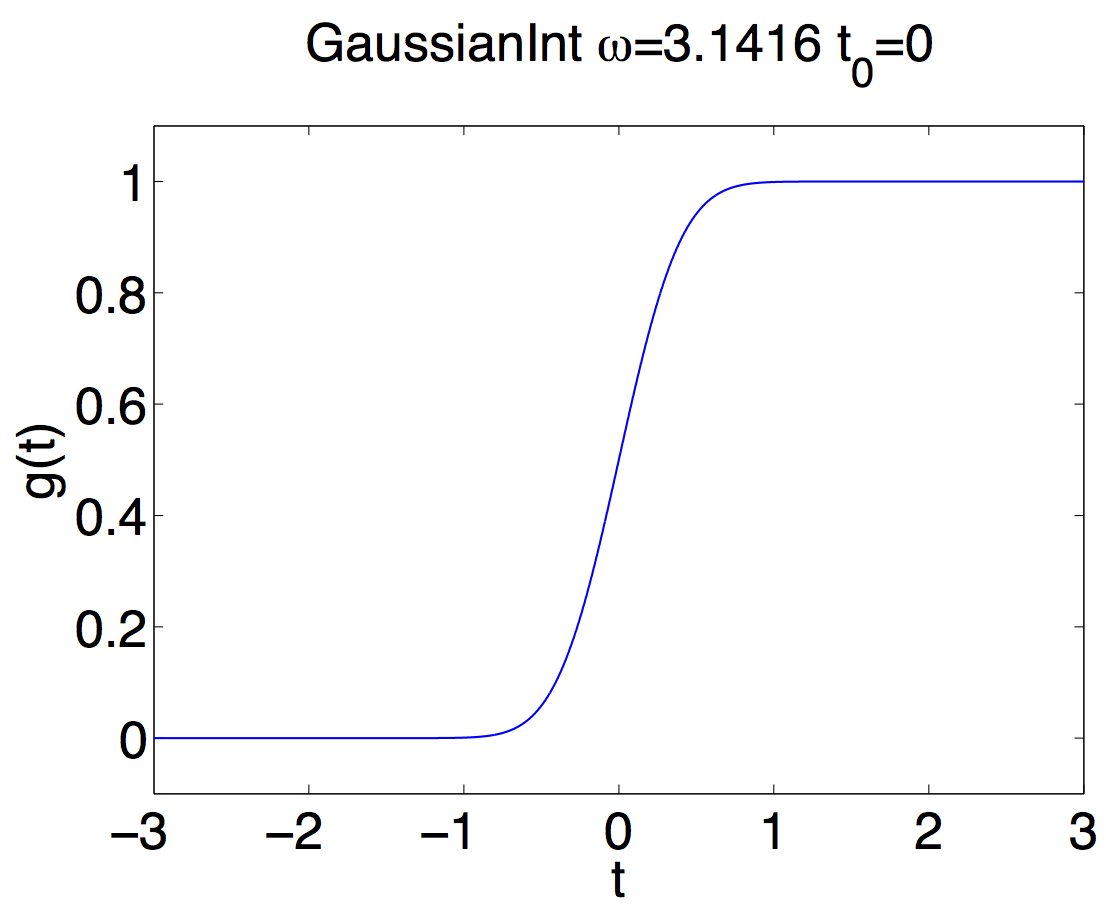
\includegraphics[width=0.4\linewidth]{f2-gaussianint.png}
  \caption{Gaussian (left) and GaussianInt (right) with $\omega=\pi$ and $t_0=0$.}
  \label{fig:gaussians}
\end{centering}
\end{figure}  
%
\subsection{Ricker} \label{ricker}
  \[
  g(t,t_0,\omega) = \left(2 \pi^2 \omega^2 (t - t_0)^2 - 1\right) e^{- \pi^2 \omega^2 (t - t_0)^2}.
  \]
A plot of the Ricker time-function is shown in Figure~\ref{fig:rickers}.

\paragraph{Important:} To avoid artifacts from a sudden startup, use
$t_0 \geq 1.35/\omega$.

\subsection{RickerInt}\label{rickerint}
  \[
  g(t,t_0,\omega) = (t - t_0) e^{- \pi^2 \omega^2 (t - t_0)^2}.
  \]
RickerInt is the time integral of the Ricker function, and is proportional to the time-derivative of
the Gaussian function. Since the RickerInt function tends to zero for large times, it does not lead
to any permanent displacements. A plot of the RickerInt time-function is shown in
Figure~\ref{fig:rickers}.
\paragraph{Important:} To avoid artifacts from a sudden startup, use
$t_0 \geq 1.35/\omega$.
\begin{figure}
\begin{centering}
  \includegraphics[width=0.4\linewidth]{f3-ricker.png}
  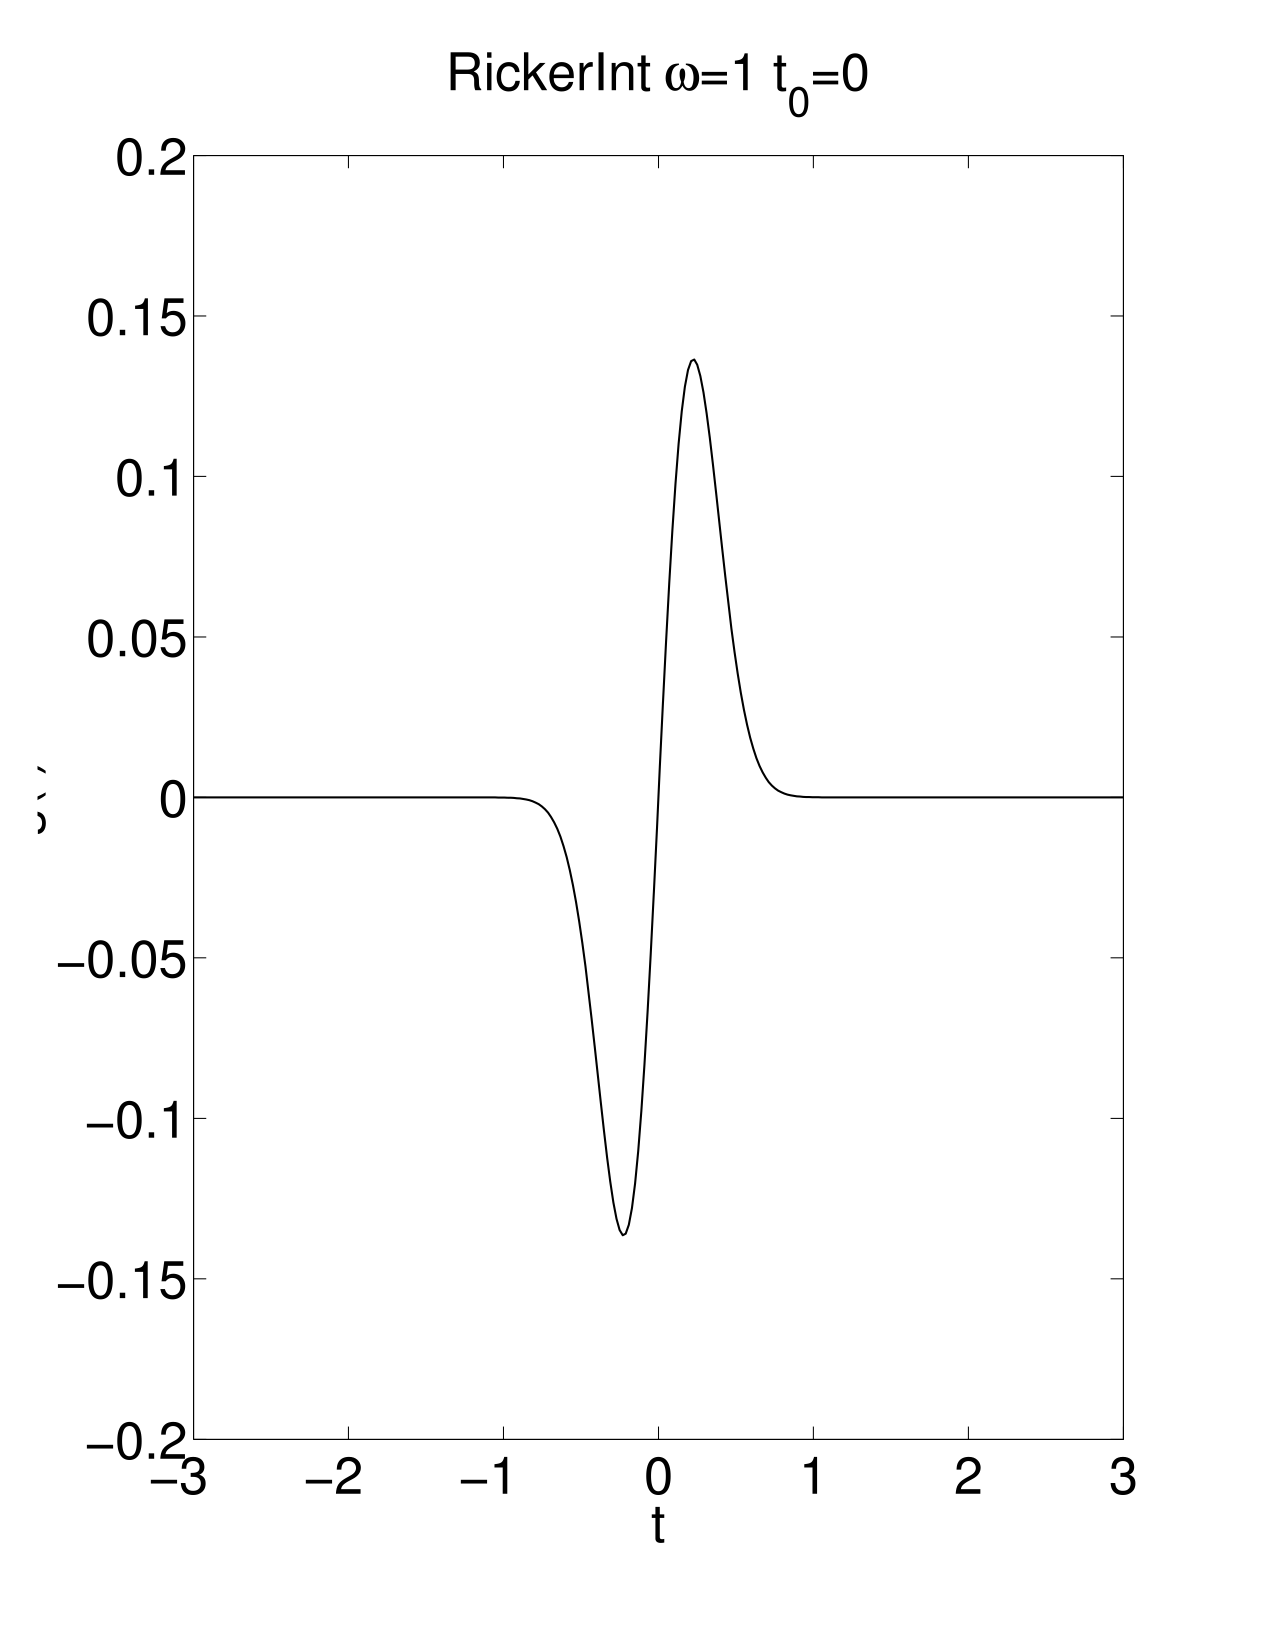
\includegraphics[width=0.4\linewidth]{f4-rickerint.png}
  \caption{Ricker (left) and RickerInt (right) with $\omega=1$ and $t_0=0$.}
  \label{fig:rickers}
\end{centering}
\end{figure}  
%
\subsection{Brune} 
 \label{brune}
\[
 g(t,t_0,\omega) = \left\{
\begin{array}{ll} 
0, & t < t_0, \\ 
1 - e^{-\omega(t-t_0)}( 1+\omega(t-t_0) ), & t \geq t_0.
\end{array}
\right.
\]
Note that the Brune function only has one continuous derivative. Because its second derivative is discontinuous at
$t=t_0$, this function can generate noisy numerical solutions. We recommend filtering all computed time
series, or using the {\bf prefilter} command to remove any unresolved motions.

\subsection{BruneSmoothed}
The BruneSmoothed function has three continuous derivatives at $t=t_0$, but is otherwise similar to
the Brune function,
\[
 g(t,t_0,\omega) = \left\{
\begin{array}{ll} 
0, & t < t_0, \\ 
1 - e^{-\omega(t-t_0)}\left[ 1+\omega(t-t_0) + \dfrac{1}{2}(\omega(t-t_0))^2\right. & \\
\quad \left.-\,\dfrac{3}{2\tau_0}( \omega(t-t_0))^3  + \dfrac{3}{2\tau_0^2}( \omega(t-t_0))^4 -
 \dfrac{1}{2\tau_0^3}( \omega(t-t_0))^5 \right], & 0< \omega (t-t_0) < \tau_0,\\
1 - e^{-\omega(t-t_0)}( 1+\omega(t-t_0) ), & \omega (t-t_0) > \tau_0.
\end{array}
\right.
\]
The parameter $\tau_0$ in the above formula is fixed to the value $2.31$. Plots of the Brune and
BruneSmoothed time-functions are shown in Figure~\ref{fig:brunes}. Since the BruneSmoothed function
has three continuous derivatives, it generates less high frequency noise than the Brune function and
gives better accuracy for a given grid resolution.
\begin{figure}
\begin{centering}
  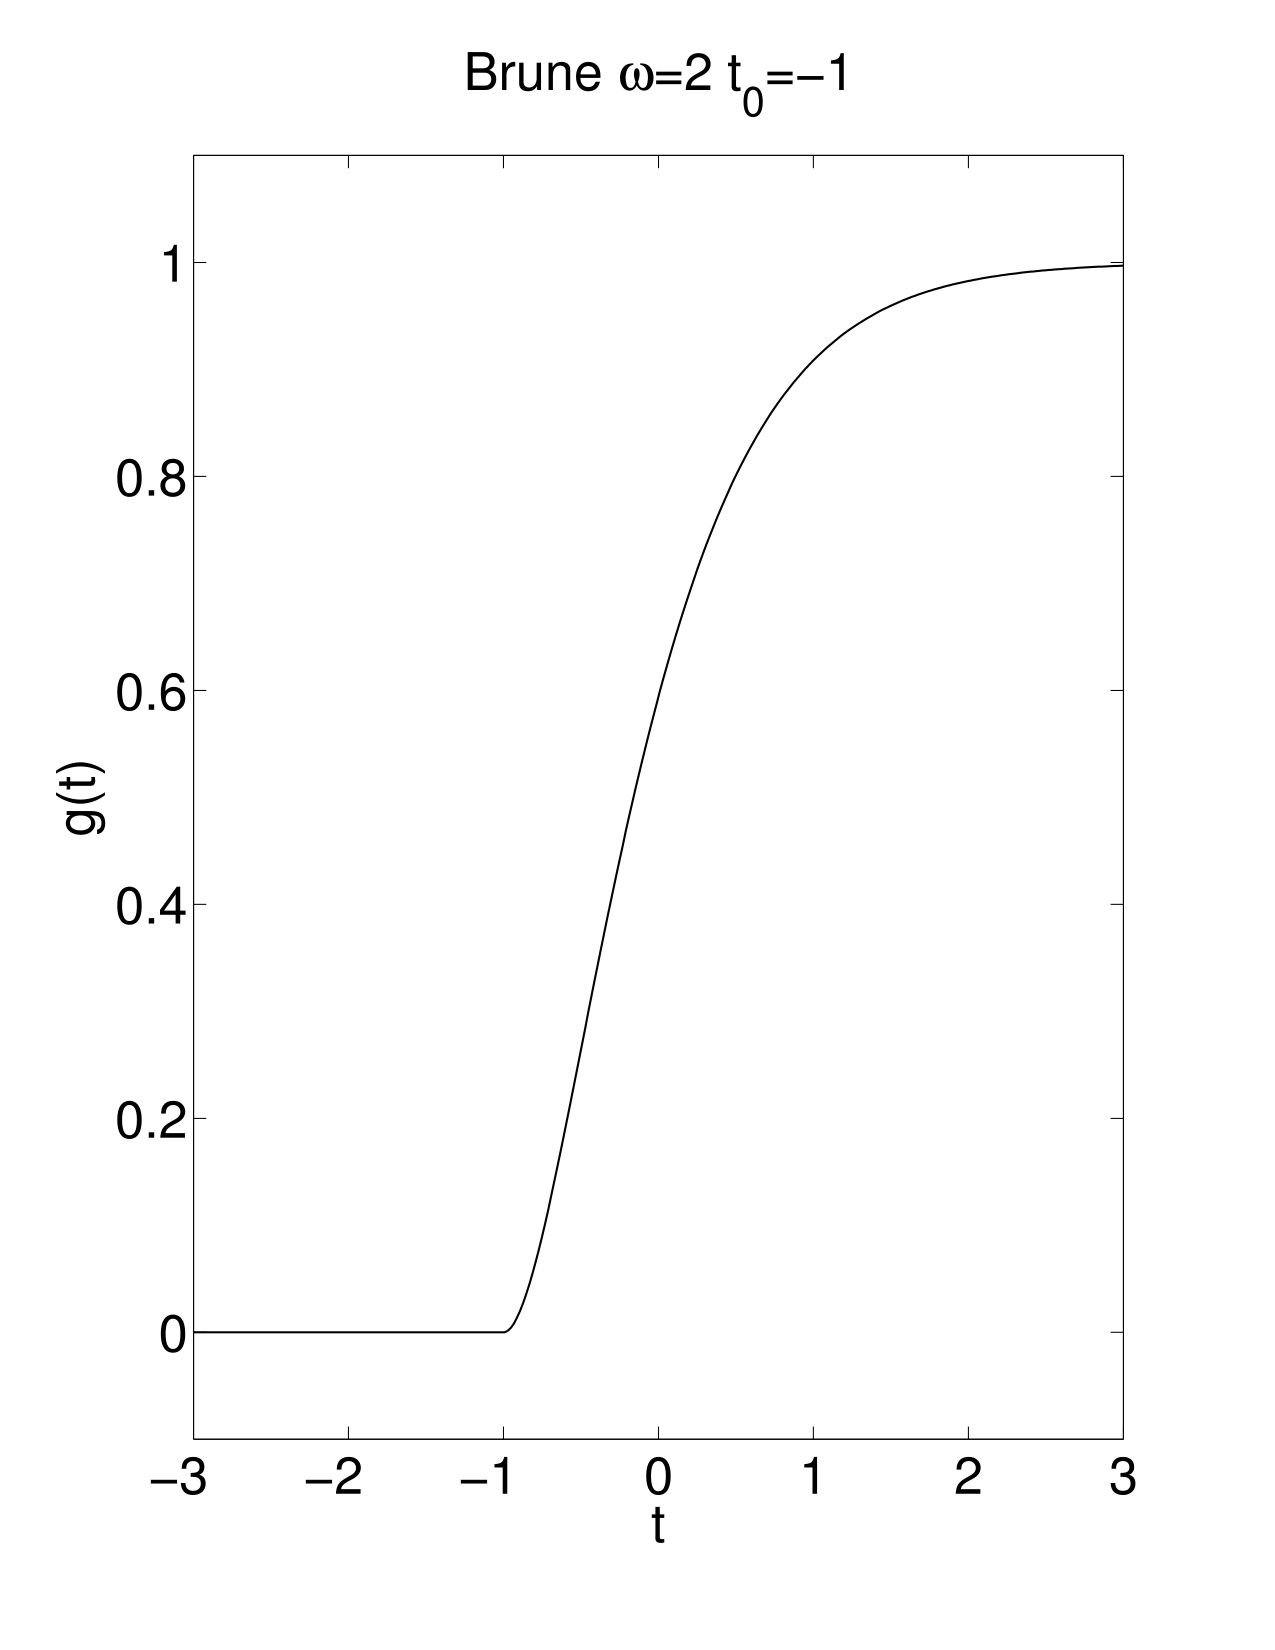
\includegraphics[width=0.4\linewidth]{f9-brune.png}
  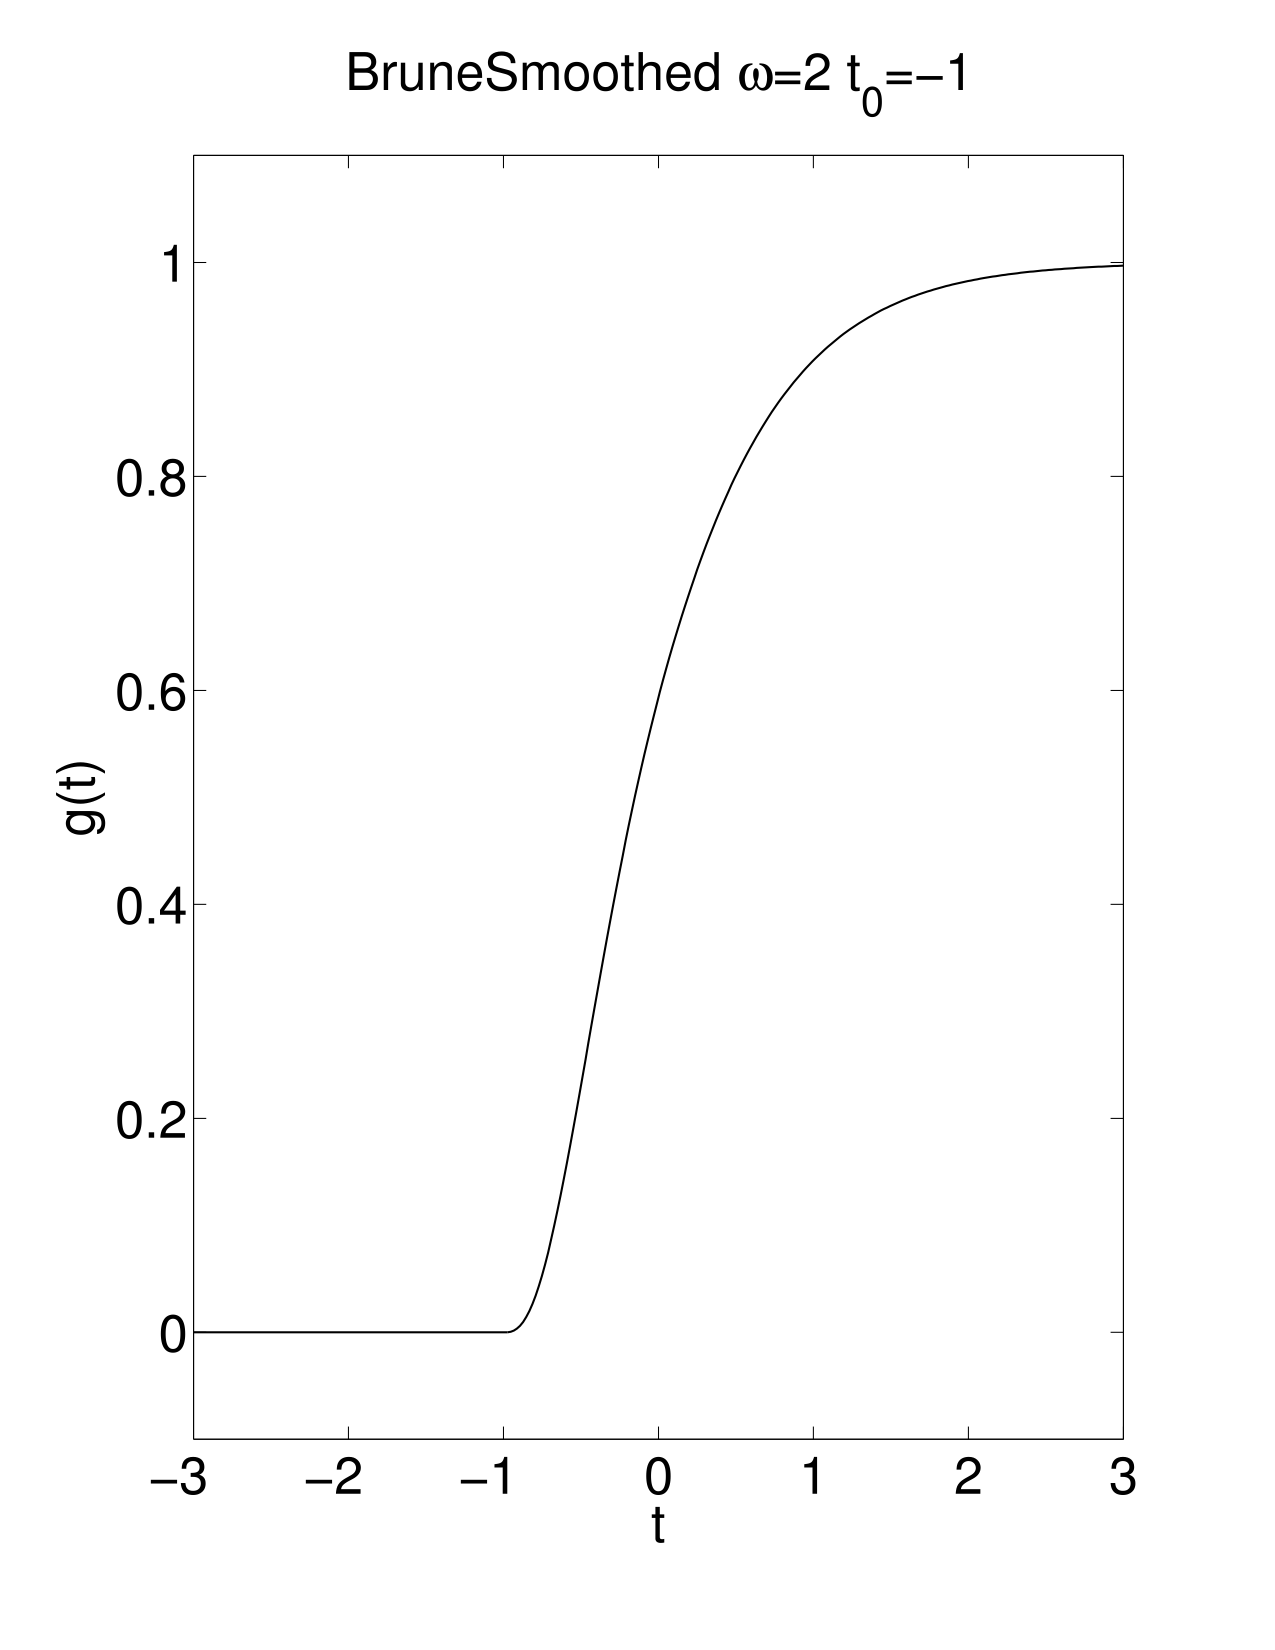
\includegraphics[width=0.4\linewidth]{f10-brunesmoothed.png}
  \caption{Brune (left) and BruneSmoothed (right) with $\omega=2$ and $t_0=-1$.}
  \label{fig:brunes}
\end{centering}
\end{figure}  

\subsection{Liu}
\renewcommand{\arraystretch}{1.5}
This function was given in the paper by Liu et al., \cite{liuetal_2006}. 
It is defined by 
\[
g(t,t_0,\omega) = \left\{ 
\begin{array}{ll}
  0, & t \leq t_0, \\
  C\left[0.7(t-t_0) + \dfrac{1.2}{\pi}\tau_1 - \dfrac{1.2}{\pi}\tau_1
  \cos\left(\dfrac{\pi (t-t_0)}{2\tau_1}\right) \right. & \\
     \hfill \left. -\,\dfrac{0.7}{\pi}\tau_1\sin\left(\dfrac{\pi (t-t_0)}{\tau_1}\right)\right],  & 
     t_0 < t \leq \tau_1+t_0, \\
%
  C\left[t-t_0-0.3\tau_1+\dfrac{1.2}{\pi}\tau_1-\dfrac{0.7}{\pi}\tau_1\sin\left(\dfrac{\pi
    (t-t_0)}{\tau_1}\right)\right. & \\ 
    \hfill
    \left. +\,\dfrac{0.3}{\pi}\tau_2\sin\left(\dfrac{\pi(t-t_0-\tau_1)}{\tau_2}\right)\right], &  
    \tau_1+t_0 < t \leq 2\tau_1+t_0, \\
%
  C\left[0.3(t-t_0)+1.1\tau_1+\dfrac{1.2}{\pi}\tau_1\right. & \\
    \hfill
    \left. +\,\dfrac{0.3}{\pi}\tau_2\sin\left(\dfrac{\pi(t-t_0-\tau_1)}{\tau_2}\right)\right], & 
    2\tau_1+t_0 < t \leq \tau+t_0, \\
  1,  &  t > \tau +t_0.
\end{array} \right.
\]
\noindent The parameters are given by $\tau=2\pi/\omega$, $\tau_1=0.13\tau$, $\tau_2 = \tau-\tau_1$,
and $C=\pi/(1.4\tau_1\pi+1.2\tau_1+0.3\tau_2\pi)$.  The Liu function resembles the Brune function,
but the rise is somewhat steeper for small $t-t_0$, see Figure~\ref{fig:liu}.
\begin{figure}
\begin{centering}
  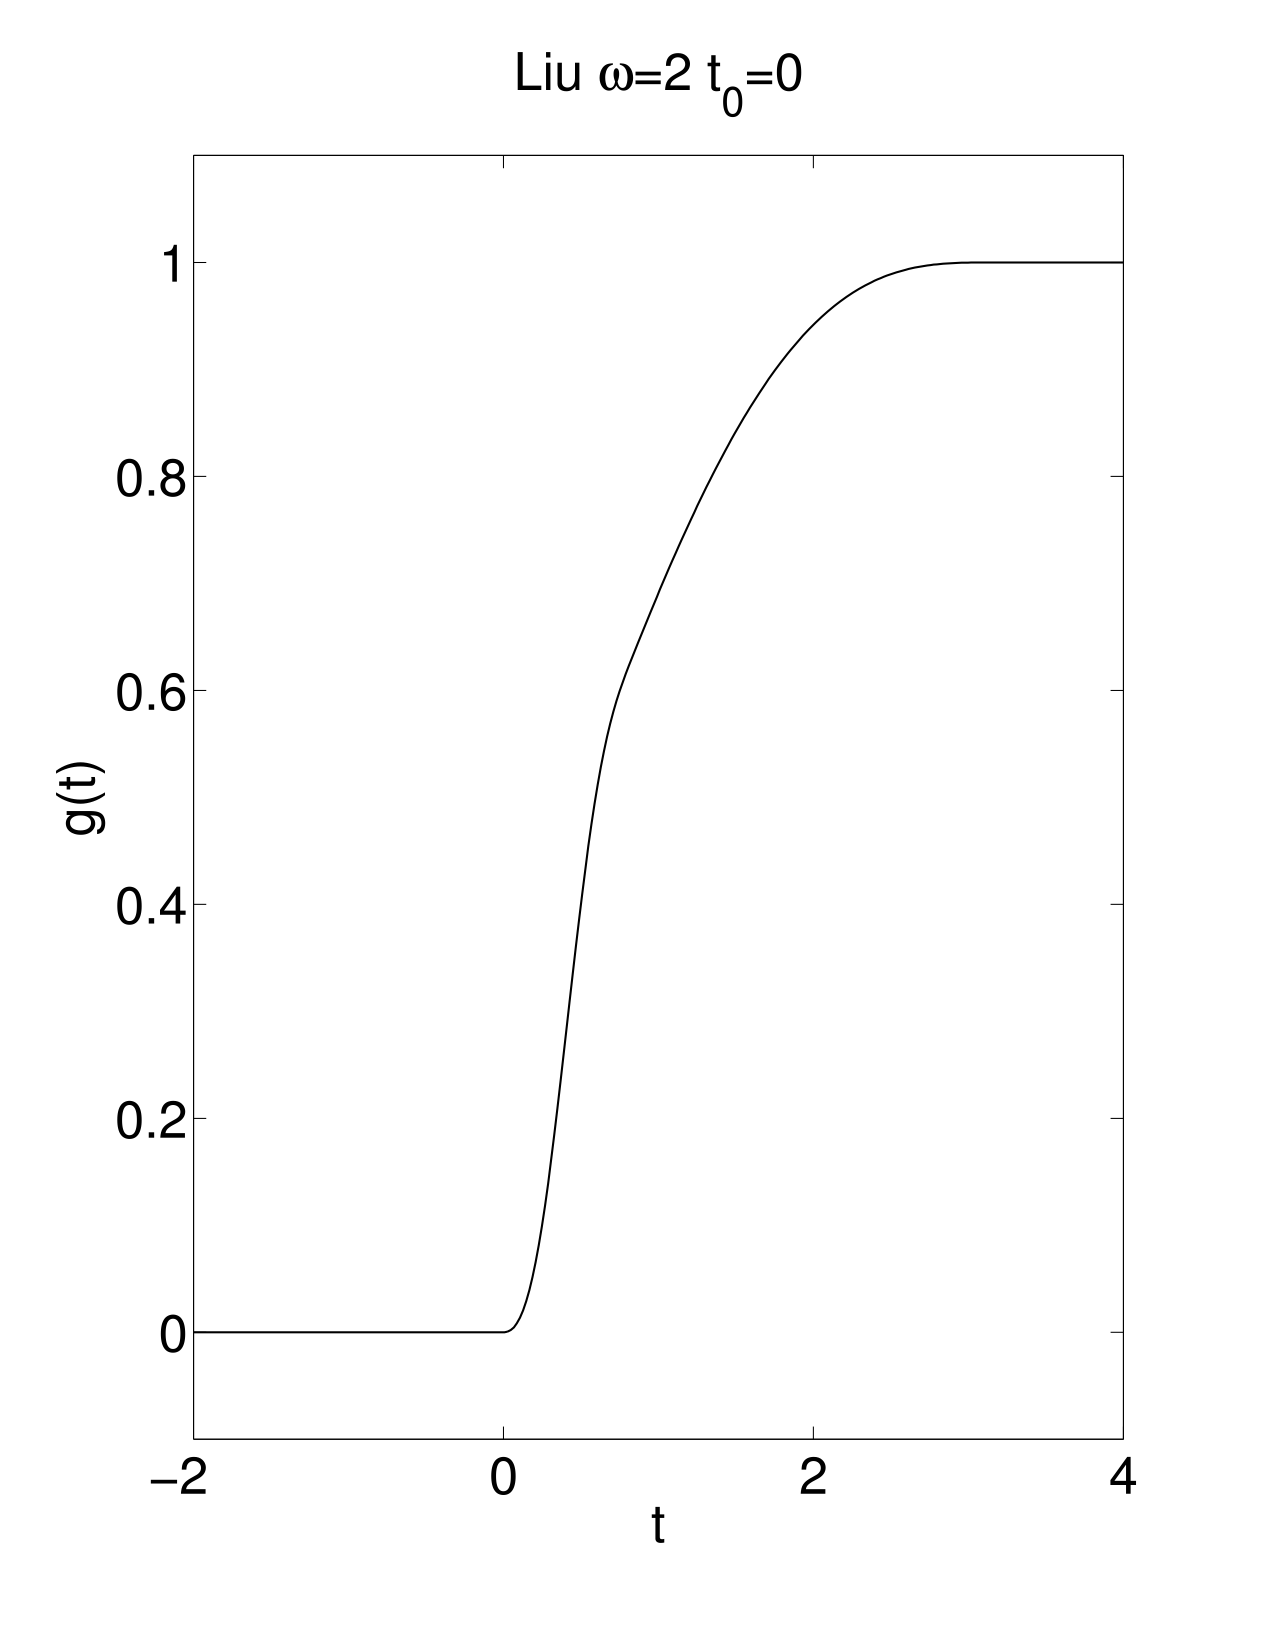
\includegraphics[width=0.4\linewidth]{f12-liu.png}
  \caption{Liu time function with $\omega=2$ and $t_0=0$.}
  \label{fig:liu}
\end{centering}
\end{figure}  

\subsection{Triangle}
\renewcommand{\arraystretch}{1.3}
For $ t_0 < t < t_0 + 1/\omega$,
\[
  g(t,t_0,\omega) = \dfrac{16 \omega}{\pi^2} \left[ \sin(\pi\omega(t - t_0)) - \dfrac{\sin(3 \pi
      \omega(t - t_0))}{9} + \dfrac{\sin(5 \pi \omega(t - t_0)}{25} - \dfrac{\sin(7 \pi \omega(t -
      t_0))}{49}\right],
\] 
with $g(t,t_0,\omega) = 0$ elsewhere. A plot of the Triangle time-function is shown in
Figure~\ref{fig:triandsaw}.
%
\subsection{Sawtooth}
For $ t_0 < t < t_0 + 1/\omega$,
\[
  g(t,t_0,\omega) = \dfrac{8}{\pi^2} \left[\sin(2 \pi \omega (t - t_0) ) - \dfrac{\sin(6 \pi
      \omega(t - t_0))}{9} + \dfrac{\sin(10 \pi \omega (t - t_0) )}{25} - \dfrac{\sin(14 \pi
      \omega(t - t_0 ))}{49}\right],
\]
with $g(t,t_0,\omega) = 0$ elsewhere.  A plot of the Sawtooth time-function is shown in
Figure~\ref{fig:triandsaw}.
\begin{figure}
\begin{centering}
  \includegraphics[width=0.4\linewidth]{f5-triangle.png}
  \includegraphics[width=0.4\linewidth]{f6-sawtooth.png}
  \caption{Triangle (left) and Sawtooth (right) with $\omega=1$ and $t_0=0$.}
  \label{fig:triandsaw}
\end{centering}
\end{figure}  
%
\subsection{Ramp}
\[ 
g(t,t_0,\omega) = \left\{ 
\begin{array}{ll} 
0, & t < t_0,\\
0.5 (1 - \cos(\pi (t - t_0) \omega)),& t_0 \leq t \leq t_0 + 1/\omega,\\
1, & t > t_0 + 1/\omega.
\end{array}
\right.
\]
A plot of the Ramp time-function is shown in Figure~\ref{fig:rampandsmoothwave}.
%
\subsection{Smoothwave}
For $ t_0 < t < t_0 + 1/\omega$,
\begin{multline*}
 g(t,t_0,\omega) = \dfrac{2187}{8} (\omega(t-t_0))^3 - \dfrac{10935}{8} (\omega(t - t_0))^4  +
  \dfrac{19683}{8} (\omega(t - t_0))^5\\ - \dfrac{15309}{8} (\omega(t - t_0))^6 +
  \dfrac{2187}{4}(\omega(t - t_0))^7,
\end{multline*}
with $g(t,t_0,\omega) = 0$ elsewhere. A plot of the Smoothwave time-function is shown in
Figure~\ref{fig:rampandsmoothwave}.
\begin{figure}
\begin{centering}
  \includegraphics[width=0.4\linewidth]{f7-ramp.png}
  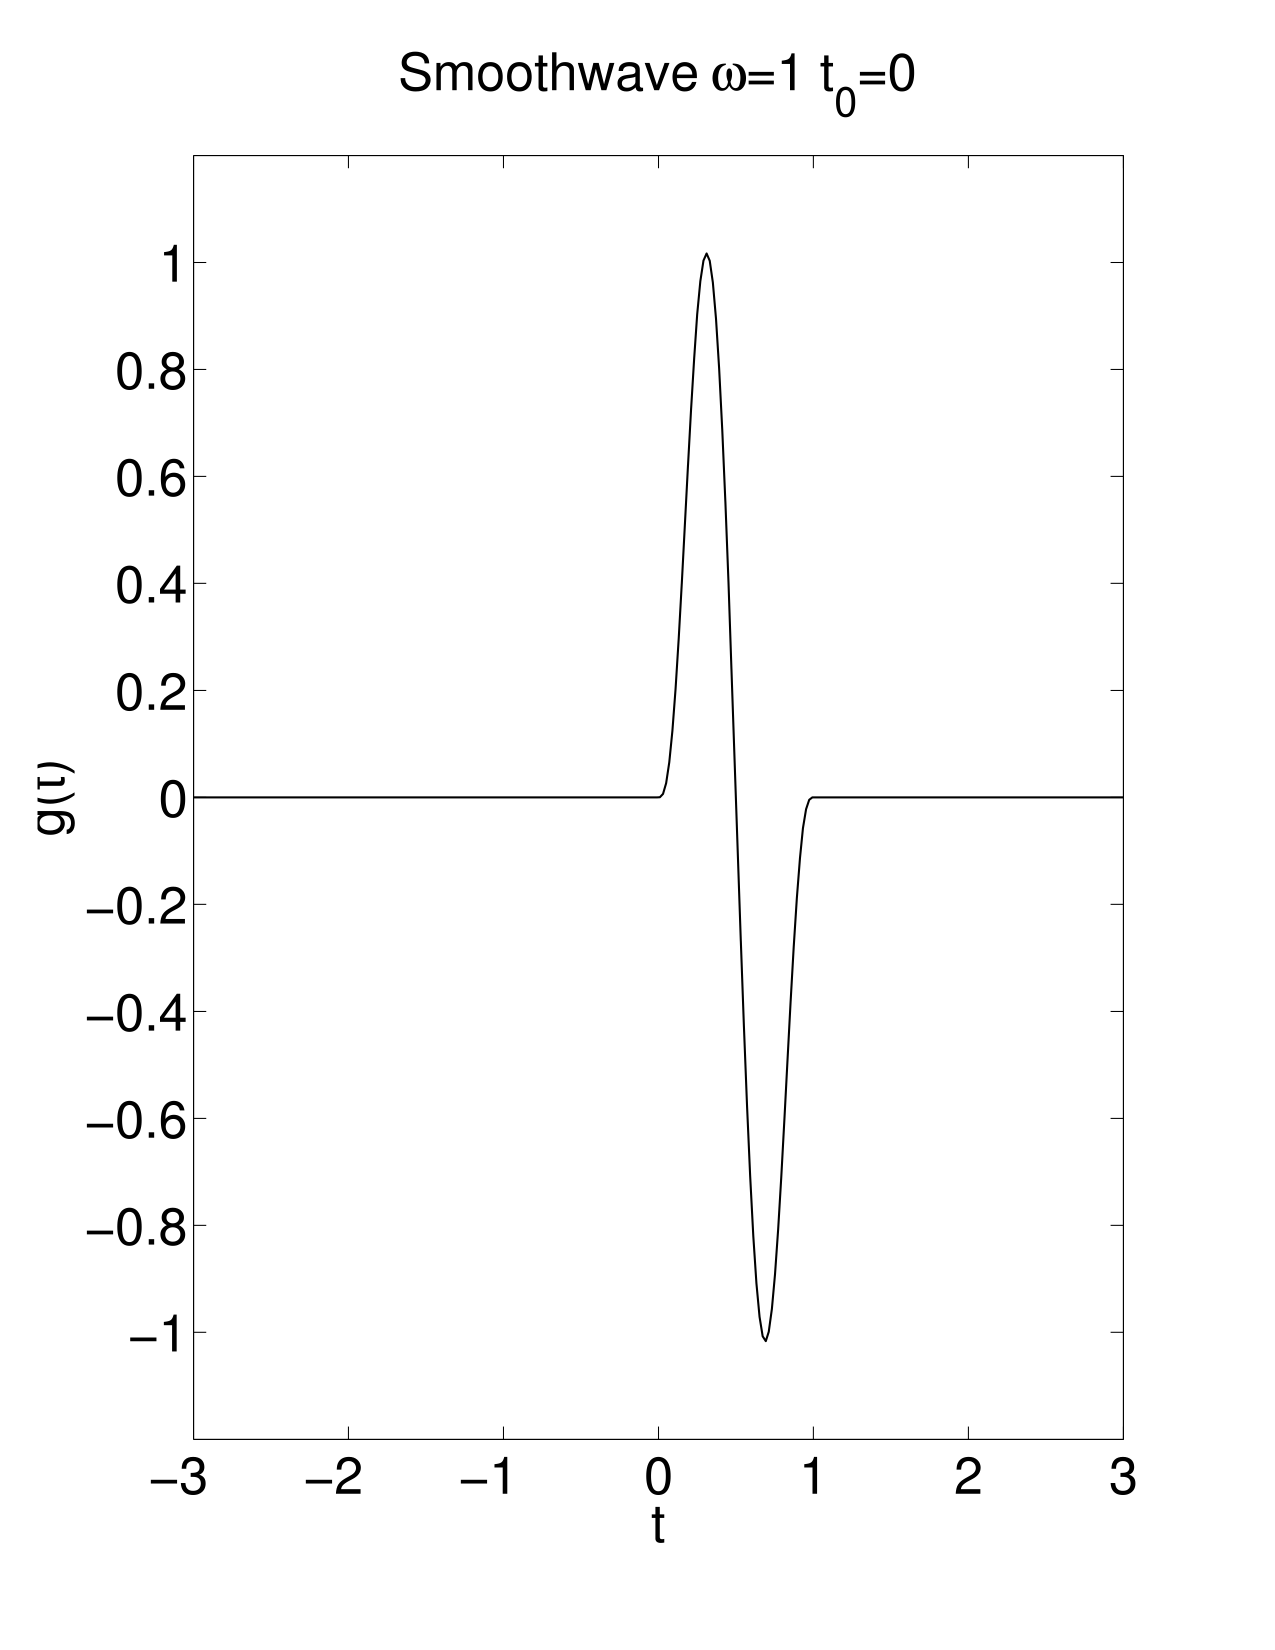
\includegraphics[width=0.4\linewidth]{f8-smoothwave.png}
  \caption{Ramp (left) and Smoothwave (right) with $\omega=1$ and $t_0=0$.}
  \label{fig:rampandsmoothwave}
\end{centering}
\end{figure}  
%
\subsection{VerySmoothBump} 
\[
g(t,t_0,\omega) = \left\{ 
\begin{array}{ll} 
0, & t < t_0,\\ 
1024\,\omega^5(t-t_0)^5 (1 - \omega(t-t_0))^5,& t_0 \leq t \leq t_0+1/\omega,\\ 
0, & t > t_0 + 1/\omega.
\end{array}
\right.
\]
The VerySmoothBump function satisfies $0\leq g\leq 1$. It has four continuous derivatives.
A plot of the VerySmoothBump time-function is shown in Figure~\ref{fig:verysmoothbump}.
\begin{figure}
\begin{centering}
  \includegraphics[height=0.4\linewidth]{f11-verysmoothbump.png}
\hspace{10mm}
  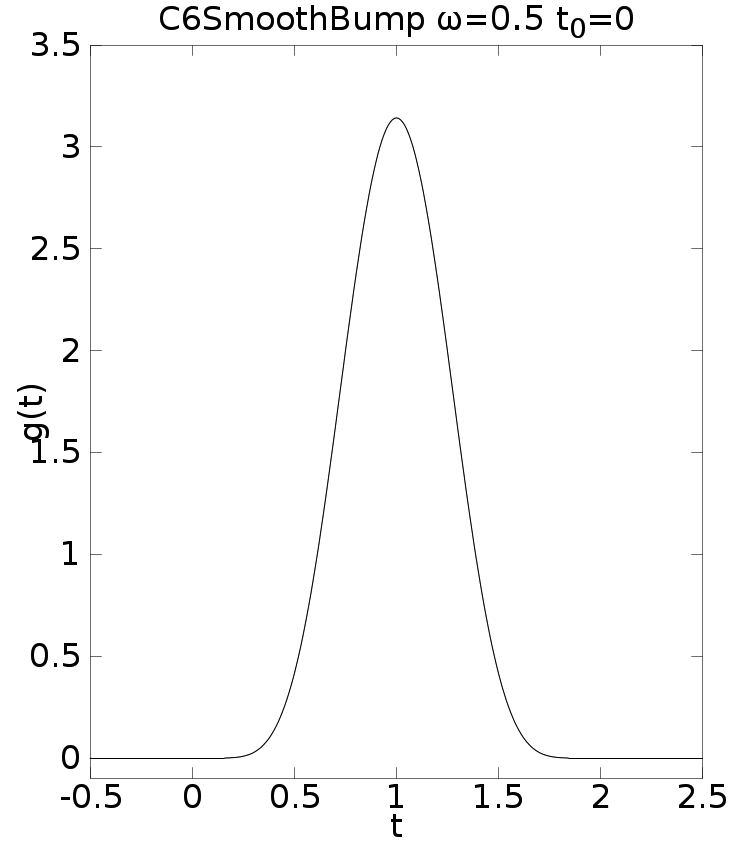
\includegraphics[height=0.4\linewidth]{f12-c6smoothbump.png}
  \caption{VerySmoothBump (left) with $\omega=0.5$ and
    $t_0=0$. C6SmoothBump (right) with $\omega=2$ and $t_0=0$.}
  \label{fig:verysmoothbump}  \label{fig:c6smoothbump}
\end{centering}
\end{figure}  
%
\subsection{C6SmoothBump} 
\[
g(t,t_0,\omega) = \left\{ 
\begin{array}{ll} 
0, & t < t_0,\\ 
51480\, \omega^7 (t-t_0)^7 (1- \omega(t-t_0))^7, & t_0 \leq t \leq t_0 + 1/\omega,\\ 
0, & t > t_0 + 1/\omega.
\end{array}
\right.
\]
The C6SmoothBump function has six continuous derivatives and integrates to one.
A plot of the C6SmoothBump time-function is shown in Figure~\ref{fig:c6smoothbump}.
%% \begin{figure}
%% \begin{centering}
%%   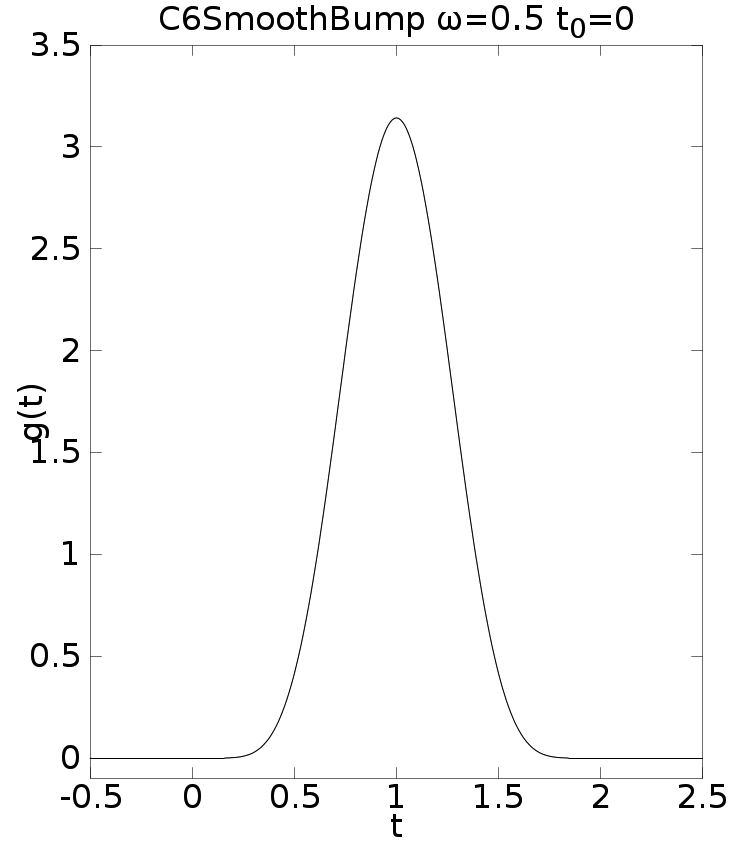
\includegraphics[width=0.5\linewidth]{f12-c6smoothbump.png}
%%   \caption{C6SmoothBump with $\omega=2$ and $t_0=0$.}
%%   \label{fig:c6smoothbump}
%% \end{centering}
%% \end{figure}  
%
\subsection{GaussianWindow}
\[
g(t,t_0,\omega) = \sin(\omega t) e^{-(\omega(t-t_0)/N_c)^2/2}
\]
A plot of the GaussianWindow time-function with $N_c=5$ is shown in
Figure~\ref{fig:gaussianwindow}. Note that $N_c$ is specified with the \verb+ncyc+ keyword, which
must be given when this time function is used in the \verb+source+ command.
\begin{figure}
\begin{centering}
  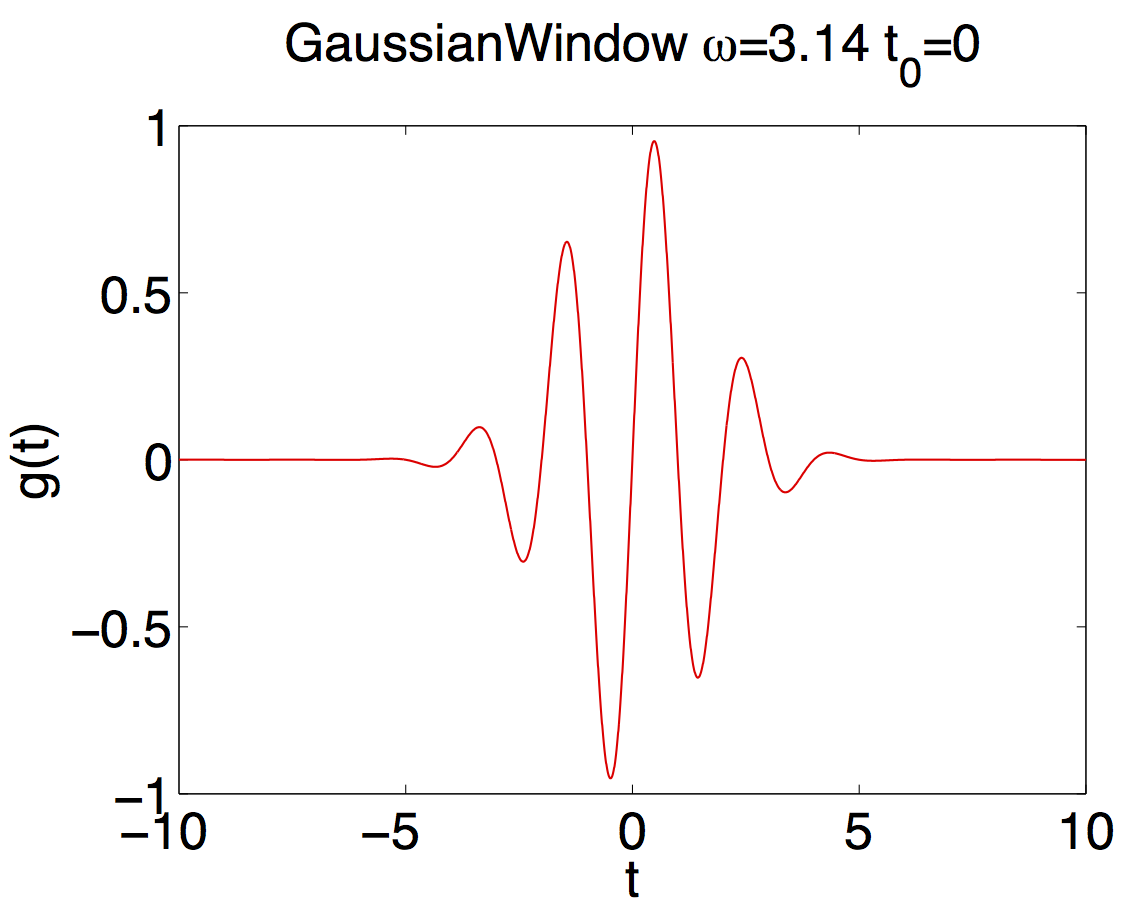
\includegraphics[width=0.6\linewidth]{GW.png}
  \caption{GaussianWindow with $\omega=3.14$, $t_0=0$, and $N_c=5$.}
  \label{fig:gaussianwindow}
\end{centering}
\end{figure}  

\subsection{Dirac}
The Dirac distribution $\delta(t-\tau_0)$ is not a regular time function because it is zero everywhere,
except at $t=\tau_0$, where it is unbounded. The integral of $\delta(t)$ is one, and if $f(t)$ is a
continuous function, then
\begin{equation}\label{eq:dirac}
\int f(t)\delta(t-\tau_0)\, dt = f(\tau_0).
\end{equation}
We discretize the Dirac distribution on a grid $t_n = n\Delta_t$, where $\Delta_t>0$ is the same
time step that is used to solve the elastic wave equation. We obtain the discrete time series $d_n$,
$n=0,1,2,\ldots$ by imposing moment conditions such that \eqref{eq:dirac} is satisfied for the
polynomial functions $f(t)=t^q$, $q=0,1,\ldots,Q$, in the sense
\[
\Delta_t \sum_{n=0}^\infty t_n^q d_n = \tau_0^q,\quad q=0,1,\ldots,Q. 
\]
This leads to $Q+1$ conditions for the coefficients $d_n$. The specification of the grid function is
made unique by enforcing $d_n=0$ except at $Q+1$ consecutive grid points surrounding $t=\tau_0$. Note
that $\tau_0$ is {\em not} required to coincide with a time step. This procedure is similar to the
spatial discretization of point force and moment tensor sources, see~\cite{PetSjo-10} for details.

The discretized Dirac distribution triggers all frequencies on the mesh, including completely
unresolved and unphysical motions. The numerical solution is therefore meaningless unless it is
filtered to remove the unresolved motions. The filtering can either be done after the simulation is
completed, or by using the {\bf prefilter} command. The Dirac time function can also be useful for
calculating ``numerical'' Green's functions.

\section{Discrete time function}

The discrete time function uses a quintic (5th order) spline function to interpolate the discrete
function values $g_j = g(\tau_j)$, for $j=1,2,\ldots, N_s$, where $N_s\geq 7$. The function values
are specified on an equidistant grid in time, $\tau_j = t_0 + (j-1) \delta_t$. The step size,
$\delta_t>0$, can be chosen independently of the time step that is used to solve the elastic wave
equation. The start time, $t_0$, can also have an arbitrary value. The interpolation procedure
results in six polynomial coefficients for each interval $\tau_j\leq t <\tau_{j+1}$. The
coefficients are chosen such that g(t) becomes four times continuously differentiable.

It is necessary to evaluate the discrete time function throughout the simulation of the elastic wave
equation, i.e., for $0\leq t\leq T$. If $\tau_1>0$, the discrete time function is evaluated using the
polynomial coefficients corresponding to the first interval $[\tau_1,\tau_2]$ for all
$0\leq t<\tau_1$. Similarily, if $\tau_{N_s}<T$, the coefficients for the last interval are used for
$\tau_{N_s}<t\leq T$. To avoid unexpected results due to extrapolation, we recommend specifying the
discrete time function for all $t\in[0,T]$. To also avoid incompatibilities between the forcing and
the homogeneous initial conditions, we recommend setting $g_j=0$ for all $\tau_j\leq 0$.

The file format for discrete time functions is decribed in~\ref{sec:discrete-time-function-format}.


\section{What is the frequency content in the time function?}\label{sec:freq}
\index{frequency content}

Figure~\ref{fig:fouriers} displays the absolute values of the Fourier transforms of the
functions Gaussian, RickerInt, Ricker, and the time derivative of the Brune
function. Inspection of the mathematical definitions of the Gaussian and Brune functions
shows that the {\tt freq} parameter specifies the angular frequency for these
functions. The relation between the fundamental frequency $f_0$ and the {\tt freq} parameter is
given by
\begin{equation}\label{eq:angular-scaling}
f_0 = \left\{ \begin{array}{ll}
 {\tt freq},& \mbox{for Ricker, RickerInt, VerySmoothBump, C6SmoothBump},\\
 \dfrac{\tt freq}{2\pi},& \mbox{for Liu, Brune, BruneSmoothed, Gaussian, GaussianInt, and GaussianWindow}.
\end{array}\right.
\end{equation}
The plots in Figure~\ref{fig:fouriers} were made with frequency parameter {\tt freq}=0.25 for the
Ricker and RickerInt functions and frequency parameter {\tt freq}=1.5 for the Gaussian and
$d/dt$(Brune) functions. Hence, $f_0\approx 0.25$ for all functions in
Figure~\ref{fig:fouriers}. Note that the Fourier
transform of the Brune function decays much slower than the other functions for high
frequencies. This is due to its lack of smoothness at $t=t_0$.
\begin{figure}
\begin{center}
\includegraphics[width=0.6\textwidth]{figfouriers.png}
\caption{ Magnitude of the Fourier transform of the derivative of the Brune (dark
  blue), the Gaussian (green), the RickerInt (red), and the Ricker (light blue)
  time-functions. Here {\tt freq}=1.5 for the Gaussian and the derivative of the Brune
  function, and {\tt freq}=0.25 for Ricker and RickerInt.}
\label{fig:fouriers}
\end{center}
\end{figure}

It is the highest significant frequency, $f_{max}$, that generates the shortest waves
and therefore determines how fine the computational grid must be. For practical purposes $f_{max}$
can be defined as the frequency where the amplitude of the Fourier transform falls below 5 \% of its
max value. We have
\begin{equation}\label{eq:upper-power-freq}
f_{max} \approx \begin{cases}
2.5 f_0,&\mbox{Ricker, RickerInt, Gaussian time functions},\\
3.0 f_0,&\mbox{C6SmoothBump time function},\\
4.0 f_0,&\mbox{Brune time function}.
\end{cases}
\end{equation}
In other words, simulations using the Brune function are the hardest to resolve on the grid and need much
more grid points to give reliable results. We remark that the Fourier transform test only makes
sense for functions that tend to zero for large times. Functions such as {\tt GaussianInt}, {\tt
  Liu}, {\tt Brune}, and {\tt BruneSmoothed} tend towards unity for large times. Their zero
frequency (DC) component therefore grows linearly with the length of the time interval, $T$. These
functions need to be differentiated before applying the above test.

The relation between the fundamental frequency $f_0$ and the highest significant frequency $f_{max}$
in (\ref{eq:upper-power-freq}) is very important. For the time functions that not are listed in that
formula, it is possible to estimate $f_{max}$ with the help of the matlab/octave scripts {\tt
  fcnplot.m} and {\tt ftfcnplot.m} in the {\tt tools} directory.

\section{How to choose the grid size} \label{sec:grid-size}
\index{grid size}

The most difficult parameter to choose when preparing the input file is probably the grid size,
$h$. It is extremely important to use a grid size that is sufficiently small, because you must resolve
the waves that are generated by the source. On the other hand you don't want to use an
unnecessarily small grid size, because both the execution time and the memory requirements
increase rapidly when the mesh is refined.

The number of grid points per shortest wavelength, $P$, is a normalized measure of how well a
solution is resolved on the computational grid. Since the shear waves and surface waves have
approximately the same wave length and propagate at approximately the same speed, we can estimate
the shortest wave length by
\[
 L_{min} = \dfrac{\min C_s}{f_{max}}.
\]
Here $C_s$ is the shear velocity of the material and $f_{max}$ is the largest significant frequency
in the time function $g(t)$, as discussed above. Hence the number of grid points per wave length
equals $L_{min}/h$, which is given by
%
\begin{equation}\label{eq:resolutionformula}
  P = \frac{L_{min}}{h} = \dfrac{\min C_s}{h\,f_{max}}. 
\end{equation}
Note that $h$ needs to be made smaller to maintain the same value of $P$ if either $C_s$ is
decreased or if the frequency is increased. In formula (\ref{eq:resolutionformula}), $\min C_s$ is
found from the material properties and $h$ is determined by the input grid specification.  The
frequency spectrum of the solution is determined by the frequency spectrum of the time
function and $f_{max}$ can be estimated from equation \eqref{eq:upper-power-freq}.

\subsection{Lamb's problem}
\label{sec:lamb}

The accuracy of the numerical solution, including the implementation of a point force and the
reflection properties of the super-grid far field boundary condition, can be tested by solving
Lamb's problem~\cite{Lamb_1904}. This problem simulates the motion due to a vertical point force
applied on the free surface of a homogeneous elastic half-space.

We have implemented Mooney's formulas~\cite{Mooney_1974} for solving Lamb's problem. These formulas
give an analytical expression for the Green's function of the vertical component along the free
surface, $z=0$. This Green's function is convolved with the source time function to give the
displacement as function of time. We use a {\tt C6SmoothBump} time function and the convolution is
performed by numerical quadrature using the Quadpack library. This approach allows the displacement
to be evaluated to within $12$ decimal places. Lamb's problem is then solved numerically using
\emph{SW4} and the error in the vertical component is evaluated along the free surface. To evaluate
how fine the grid needs to be, we repeat the test for different grid sizes. See Petersson and
Sjogreen~\cite{PetSjo-13} for further details.

% 2nd example
In this example, the elastic half-space consists of a homogeneous material with shear wave
velocity $C_s=1000$ m/s, compressional wave velocity $C_p=1000\sqrt{3}$ m/s, and density $\rho=1500$
kg/m$^3$. The elastic half-space is truncated to the computational domain
\[
(x,y,z) \in [0,10000] \times [0,10000]\times[0,5000].
\]
The source is placed on the free surface in the center point of the horizontal plane:
$(5000,5000,0)$. The time dependency of the forcing is a ``C6SmoothBump'' (see Figure
\ref{fig:c6smoothbump}) with $\omega=1$ Hz, $t_0=0$ s and magnitude $10^{13}$ N. The above setup is
created with the input file shown below, which can be found in {\tt examples/lamb/seismic1.in}
\begin{verbatim}
grid nx=151 x=10e3 y=10e3 z=5e3
time t=5.0
supergrid gp=60
block vp=1.7320508076e+03 vs=1000 rho=1500
source type=C6SmoothBump x=5e3 y=5e3 z=0 fz=1e13 freq=1 t0=0
rec x=5e3 y=6e3 z=0 file=v1 sacformat=0 usgsformat=1
\end{verbatim}
Because the frequency parameter of the {\tt C6SmoothBump} time function is $f_0=1$ Hz and $C_s=1000$
m/s, the dominant wave length in the solution is about 1,000 meters. Hence the receiver is located
approximately one wave length from the source.

It is well known that the error in numerical solutions of wave propagation problems is dominated by
phase errors~\cite{Gustafsson-Kreiss-Oliger}. It is therefore interesting to investigate how the
accuracy in the numerical solution depends on the distance between the source and receiver. For this
reason, we expand the above calculation to include a second receiver at distance 10,000 meters from
the source. This input file is given in {\tt examples/lamb/seismic2.in}. In this case, we evaluate
the solution of Lamb's problem using the Fortran program {\tt src/lamb\_one\_point.f}. The vertical
displacements and errors are shown in Figure~\ref{fig:lambSAC}.
\begin{figure}[ht]
  \begin{center}
    \includegraphics[width=0.9\textwidth]{lamb-err-h66.png}
    \caption{Lamb's problem: Vertical displacement at 1,000 (blue) and 10,000 (red) meters from the
      source. The green and light blue lines show the corresponding errors in the
      numerical solution with $h=200/3$, corresponding to $P=5$ grid points per shortest wave
      length. The displacement is offset by 1 for the second recording.}
    \label{fig:lambSAC}
  \end{center}
\end{figure}
The waveforms are smooth and the problem appears to be well resolved. Because of geometric
spreading, the amplitude of the exact solution decreases with the distance from the source. At the
same time, the amplitude of the error increases. This is because the numerical solution accumulates
discretization errors as it propagates through the computational grid.

We show the errors in the vertical displacement in Table~\ref{tab:lamb-err}. The errors are
presented in max norm, normalized by the max norm of the exact solution. The
frequency parameter in the {\tt C6SmoothBump} time function is $f_0=1$ Hz. Following
(\ref{eq:upper-power-freq}), we estimate the highest significant frequency to be $f_{max}=3.0$
Hz. In this case the formula for the number of grid points per wave length
(\ref{eq:resolutionformula}) becomes
\[
P=\frac{1000}{3 h}.
\]
Also note how quickly the total number of grid points ($N_{GP}$) increases when the grid is
refined. 

The errors are also plotted in Figure~\ref{fig:ppw-err}.
\begin{table}
\begin{center}
\begin{tabular}{| c | c | c | c | c |}
\hline
$h$ & $P$  & $\| e_1^{(z)}\|_\infty / \|U_1^{(z)}\|_\infty$  & $\| e_{10}^{(z)}\|_\infty /
\|U_{10}^{(z)}\|_\infty$ & $N_{GP}$ \\ \hline
 200/3 & 5   & $7.17\cdot 10^{-2}$  & $4.31\cdot 10^{-1}$ & $3.0\cdot 10^7$ \\ \hline
 50    & 6.7 & $3.44\cdot 10^{-2}$  & $2.43\cdot 10^{-1}$ & $7.3\cdot 10^7$ \\ \hline
 100/3 & 10  & $9.31\cdot 10^{-3}$  & $6.99\cdot 10^{-2}$ & $2.4\cdot 10^8$ \\ \hline
 25    & 13.3 & $3.25\cdot 10^{-3}$ & $2.42\cdot 10^{-2}$ & $5.8\cdot 10^8$ \\ \hline
\end{tabular}
\caption{Lamb's problem: Relative max norm errors in the vertical displacement at $1,000$ and
  $10,000$ meters from the source. Here, $h$ is the grid size, corresponding to $P$ grid points per
  shortest wave length. Also, $N_{GP}$ is the total number of grid points in the 3-D grid.}
\label{tab:lamb-err}
\end{center}
\end{table}
The error decreases at a rate approaching ${\cal O}(h^4)$ for the finest grid, indicating that the
numerical method and the discretization of the point force are fourth order accurate.
\begin{figure}[htp]
\begin{centering}
  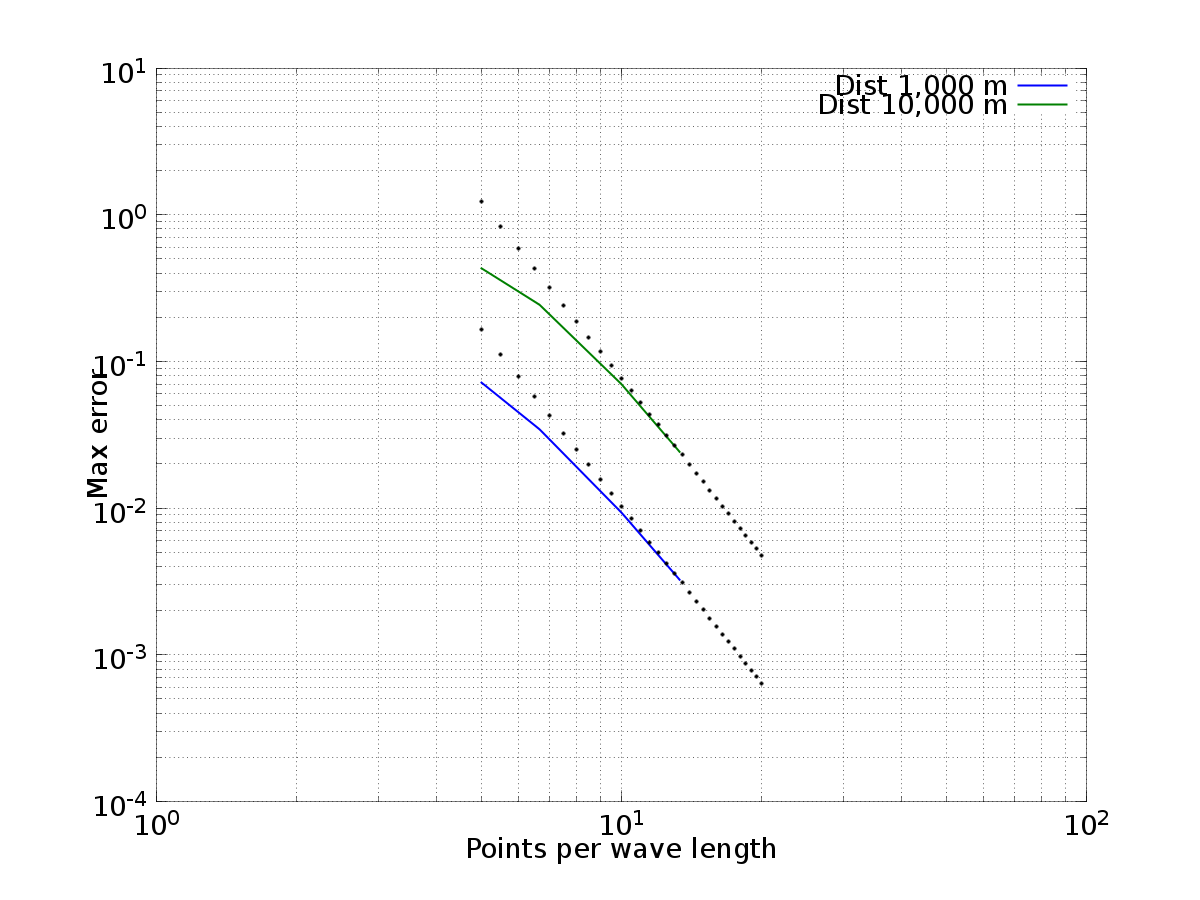
\includegraphics[width=0.8\linewidth]{ppw-err.png}
  \caption{Lamb's problem: Error in max norm as function of the number of points per wave length at
    1,000 meters (blue) and 10,000 meters (green) from the source. The
    dotted lines indicate the asymptotic decay of the error in a fourth order accurate method.}
  \label{fig:ppw-err}
\end{centering}
\end{figure}
For the same grid size, note that the error is about 7.5 times larger at 10 km from the source,
compared to 1 km. To get the same accuracy at 10 km from the source, the grid size must be reduced
by a factor of $(7.5)^{1/4}\approx 1.65$, i.e., the number of grid points per wave length must be
increased by the same factor.

From this experiment we conclude that the accuracy in \emph{SW4} depends on the distance between the
source and the reciever, which can be normalized by the dominant wave length in the solution. For
most practical purposes the accuracy is acceptable when
\[
6 \leq P \leq 12,
\]
but the exact number depends on the required accuracy. The ratio between the compressional and shear
velocity, $C_p/C_s$, can also have a significant influence on the accuracy of the solution, and the
number of grid points per wave length must be increased for materials with large
$C_p/C_s$, see~\cite{KrePet-12}. 

We finally remark that the best way of checking the accuracy in a numerical simulation is to repeat
the calculation on a finer mesh and compare the results. Unfortunately, this approach is seldomly
used in realistic situations because the computational cost increases too rapidly as the mesh is refined.

%%%%%%%%%%%%%%%%%%%%%%%%%%%%%%%%%%%%%%%%%%%%%%%%
\chapter{Topography} \label{sec:topography}
\index{topography}
%%%%%%%%%%%%%%%%%%%%%%%%%%%%%%%%%%%%%%%%%%%%%%%%

The topography command in \emph{SW4} is used to specify the shape of the top surface of the
computational domain,
\[
z=\tau(x,y).
\]
Three different topography descriptions are currently implemented in \emph{SW4}: a Gaussian hill
(\S~\ref{sec:topo-gauss-hill}), a latitude-longitude grid file (\S~\ref{sec:topo-gridfile}), or
topography from an Etree database (\S~\ref{sec:topo-efile}).

A curvilinear grid is automatically constructed between the topography surface and a user specified depth
$z=$\verb+zmax+. If no topography command is present in the input file, the top surface is taken to
be the plane $z=0$, and no curvilinear grid is constructed. If the topography surface $z=\tau(x,y)$ varies between
$\tau_{min}\leq z\leq \tau_{max}$ ($z$ is positive downwards), the grid generation usually works well if
\begin{equation}\label{zmax-limit}
\mbox{\tt zmax} \geq \tau_{max} + 2(\tau_{max}-\tau_{min}),
\end{equation}
After reading the topography, \emph{SW4} prints out the min and max $z$-coordinates, as well as the
specified value of \verb+zmax+,
\begin{verbatim}
***Topography grid: min z = -1.1443e+03, max z = 1.0929e+03, \
   top Cartesian z = 6.000000e+03
\end{verbatim}
This case corresponds to the topography shown in Figure~\ref{fig:efile-topo},
\[
\tau_{min} = -1144.3, \quad \tau_{max} = 1092.9,
\]
and \verb+zmax=+ 6000.  We have $\tau_{max} + 2(\tau_{max}-\tau_{min})=5567.3$, which satisfies \eqref{zmax-limit}.
%
\begin{figure}[htp]
  \begin{center}
    \includegraphics[width=0.7\textwidth]{efile-topo.png}
    \caption{Topography and bathymetry in the
      vicinity of San Jose, south of San Francisco. The coastline is outlined by a thicker black
      line. Note the deep water in the Monterey Canyon, near the bottom corner of the computational domain. }
    \label{fig:efile-topo}
  \end{center}
\end{figure}
%

Except for the Gaussian hill topography, the topography surface is smoothed by a Jacobi iteration
before the curvilinear grid is generated,. The purpose of the smoothing is to ensure that the
variations in topography can be resolved on the computational grid. By default, 10 iterations are
performed and this gives a satisfactory result in many cases. It is possible to change the number of
iteration by using the \verb+smooth+ option in the topography command. You can inspect the result of
the smoothing by saving the top grid surface in an image file,
\begin{verbatim}
image mode=grid z=0 cycle=0 file=test
\end{verbatim}
Note that the $z$ coordinate (positive downwards) is saved on a grid image file, while the elevation
(positive upwards) of the raw (before smoothing) topography is saved on a topo image file.

\section{Gaussian hill topography}\label{sec:topo-gauss-hill}
The simplest type of topography is a Gaussian hill, allowing the user to place one Gaussian hill at
a specified location in the $(x,y)$-plane. The user can adjust the amplitude of the hill as well as
its spread in the $x$ and $y$-directions. The Gaussian hill topography command has the following
syntax:
\begin{verbatim}
topography input=gaussian zmax=7.5 gaussianAmp=2.4 \
           gaussianXc=3.6 gaussianYc=2.4 \
           gaussianLx=0.25 gaussianLy=0.3
\end{verbatim}
Note the \verb+zmax+ option, which tells \emph{SW4} to extend the curvilinear grid to $z=7.5$.
The most common use of the Gaussian hill topography is for testing, see for example the input
scripts in \verb+examples/twilight+:
\begin{verbatim}
gauss-twi-1.in  gauss-twi-2.in  gauss-twi-3.in 
\end{verbatim}

\section{Topography grid file}\label{sec:topo-gridfile}
The topography can be given on a regular lattice in geographical (lat, lon), or Cartesian $(x, y)$
coordinates. This approach works well together with the \verb+block+, \verb+pfile+, and \verb+ifile+
material commands. It can also be used together with the \verb+efile+ command, but in that case it is important
that the topography is consistent with the etree database, see Section~\ref{sec:topo-efile}.

To setup the topography, you can give the command
% for the Grenoble basin test case described in
% Section~\ref{sec:grenoble}, you 
\begin{verbatim}
topography input=grid file=grenobleCoarse.topo zmax=3000 order=2
\end{verbatim}
The file \verb+grenobleCoarse.topo+ holds the elevation (in meters) relative to mean sea level and
must conform to the simple ASCII text format described in Section~\ref{sec:ifile-format}. In the
above case, a curvilinear grid is constructed between the topography surface and $z=3000$, and the
\verb+order=2+ option specifies a second order polynomial stretching in the curvilinear mapping
function. The topography is shown in Figure~\ref{fig:grenoble-topo}.
%
\begin{figure}[htp]
  \begin{center}
    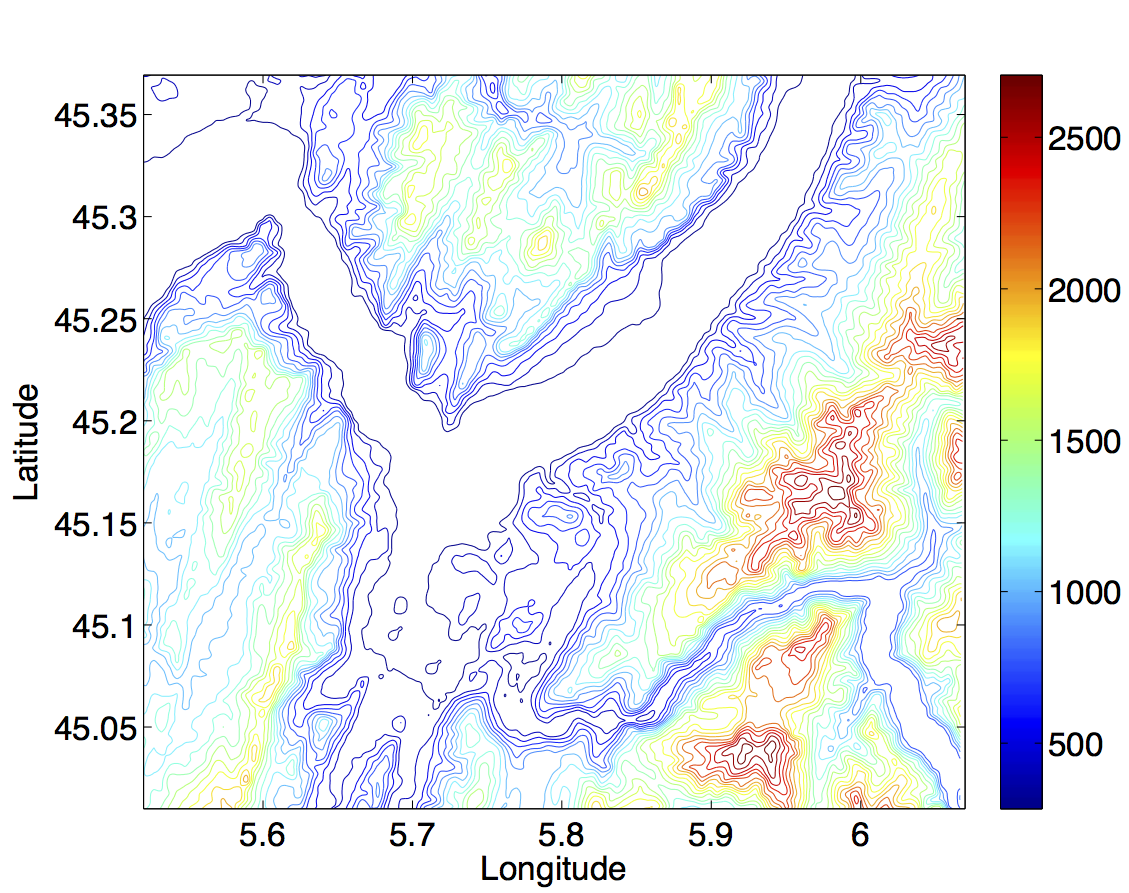
\includegraphics[width=0.7\textwidth]{grenoble-topo.png}
    \caption{Topography in the vicinity of Grenoble, France.}
    \label{fig:grenoble-topo}
  \end{center}
\end{figure}

\section{Etree topography}\label{sec:topo-efile}

The Etree databases for the San Francisco bay area and Northern California contain topographic
information. You can setup the computational grid to follow this topography by using the following command,
\begin{verbatim}
topography input=efile etree=USGSBayAreaVM-08.3.0.etree zmax=6e3 order=3
\end{verbatim}
Note that the syntax has been changed from \emph{WPP}. Here, the topography command tells \emph{SW4}
to read the topography from the specified Etree file. The \verb+etree+ keyword can also be called
\verb+file+. The \verb+order=3+ option specifies the type of stretching to use when making the
curvilinear grid. A higher value makes the curvilinear grid smoother near the bottom, but can cause
a larger variation in grid size near the top. The \verb+zmax=6e3+ option tells \emph{SW4} to put the
bottom boundary of the curvilinear grid at $z=6000$.

When the computational domain is larger, it is possible to combine the topographic information from
the detailed and regional databases, using the following syntax:
\begin{verbatim}
topography input=efile etree=USGSBayAreaVM.etree xetree=USGSBayAreaVMExt.etree \
           zmax=6e3 order=3
\end{verbatim}
Here the filenames have been abbreviated to improve readability.


%%%%%%%%%%%%%%%%%%%%%%%%%%%%%%%%%%%%%%%%%%%%%%%%
\chapter{The material model} \label{sec:material}
\index{material}
%%%%%%%%%%%%%%%%%%%%%%%%%%%%%%%%%%%%%%%%%%%%%%%%

The elastic material model in \emph{SW4} is defined by the grid point values of the density
($\rho$), the compressional velocity ($V_p$), and the shear velocity ($V_s$). The material
properties can be specified by the \verb+block+ command (\S~\ref{sec:block}), the \verb+efile+ command
(\S~\ref{sec:efile}), the \verb+pfile+ command (\S~\ref{sec:pfile}), the \verb+ifile+ command
(\S~\ref{sec:ifile}), or by a combination of them. If the same computational grid is used for
several simulations, the material model can also be obtained through the \verb+vimaterial+ command,
assuming that it was initially saved using the \verb+volimage+ command. See \S~\ref{sec:vimat} for
details.

This chapter only discusses elastic materials. See chapter~\ref{sec:attenuation} for visco-elastic
material models.


Note that \emph{SW4} uses two layers of ghost points outside the computational domain (as defined by
the grid command). The material properties must therefore be defined for the computational domain
padded by two layers of ghost points (one layer above the free surface boundary). If the material
model is not defined in these ghost points, it will be extrapolated from the nearest boundary. Note
that this behavior is different from \emph{WPP}, which requires the user to also define the material in
the ghost points.

The order within the material commands (block, pfile, efile, and ifile) {\em does} matter (unlike
all other commands) in that the priority of the material command increases towards the end of the
input file. Hence, a material command in the input file can be completely or partially overridden by
subsequent material commands.

In the block, pfile, and ifile commands, material properties are assigned based on the depth below
the free surface. This means that the internal material model depends on the topography, but the
material properties along the free surface will always be the same, independent of the topographic
model. For the efile command, material properties are defined as functions of elevation relative to
mean sea level ($z=0$). In this case the topography information is embedded in the material
description. If you combine the efile command with a planar topography, a linear mapping is
constructed before the material properties are assigned. The properties at the free surface are thus
mapped to the top grid surface ($z=0$), and the bottom grid surface (with $z=z_N$) is assigned
material properties for elevation $-z_N$. Elevation values at intermediate grid points follow from
the linear mapping.
%The material properties in the coarser Cartesian grids are not effected
%by this mapping procedure.

After reading all material commands in the input file and assigning material properties to the
computational grid, \emph{SW4} outputs general information about the ranges in the material
model. For a purely elastic material, the output looks like
\begin{verbatim}
       ----------- Material properties ranges ---------------
       1590 kg/m^3 <=  Density <= 3300 kg/m^3
       768 m/s    <=  Vp      <= 7790 m/s
       500 m/s    <=  Vs      <= 4420 m/s
       1.536        <=  Vp/Vs   <= 4.48
       3.975e+08 Pa     <=  mu      <= 6.44701e+10 Pa
       1.4282e+08 Pa     <=  lambda  <= 7.13863e+10 Pa
       ------------------------------------------------------
\end{verbatim}
It is always a good idea to check that these numbers are reasonable before proceeding with the
simulation. In addition, we recommend inspecting the material model along a few \verb+image+ planes.

Before the simulation is started, \emph{SW4} checks that density, $V_p$, and $V_s$ are
positive at all grid points. In addition, it is verified that the first Lam\'e parameter satisfies
$\lambda>0$, that is $V_p/V_s > \sqrt{2}$. If either of these conditions is violated, the program
stops with an error message. You can obtain more detailed diagnostics by setting \verb+verbose=3+
(or higher) in the \verb+fileio+ command.


%%%%%%%%%%%%%%%%%%%%%%%%%%%%%%
\section{The block command}\label{sec:block}
%%%%%%%%%%%%%%%%%%%%%%%%%%%%%%
The block command can be used to specify material properties in rectangular volumes of the
computational domain, either with constant values or linear vertical gradients. By combining the
block command with the sub-region options we can define a material model composed of three layers:
\begin{verbatim}
block vp=4000 vs=2500 rho=2000 
block vp=6000 vs=3500 rho=2700 z1=15000
block vp=8000 vs=4500 rho=3300 z1=35000 z2=100000
\end{verbatim}
In this case the top layer has a thickness of 15 km, the middle layer 20 km and the lower layer 65 km. Because
these block commands do not specify horizontal coordinates, the values extend to the grid boundaries in
both horizontal directions.  To add a box shaped inclusion of a new material we could add the following line
\begin{verbatim}
block vp=3000 vs=2000 rho=1000 \ 
      x1=4000 x2=8000 y1=3000 y2=7000 z1=10000 z2=70000
\end{verbatim}
\begin{figure}[ht]
\begin{centering}
  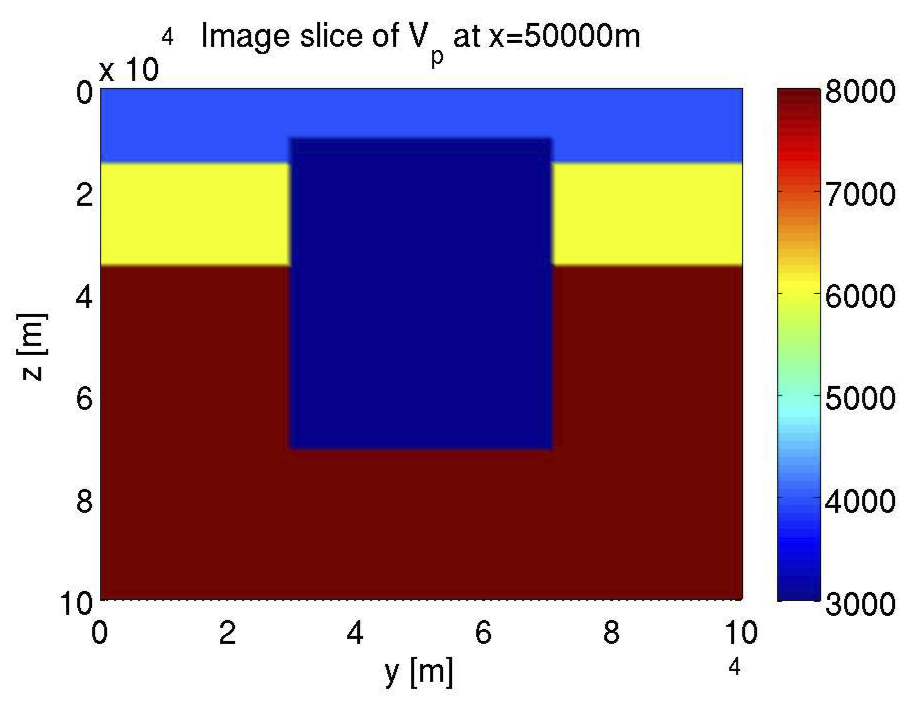
\includegraphics[width=0.45\linewidth]{blockVpimage.png}
  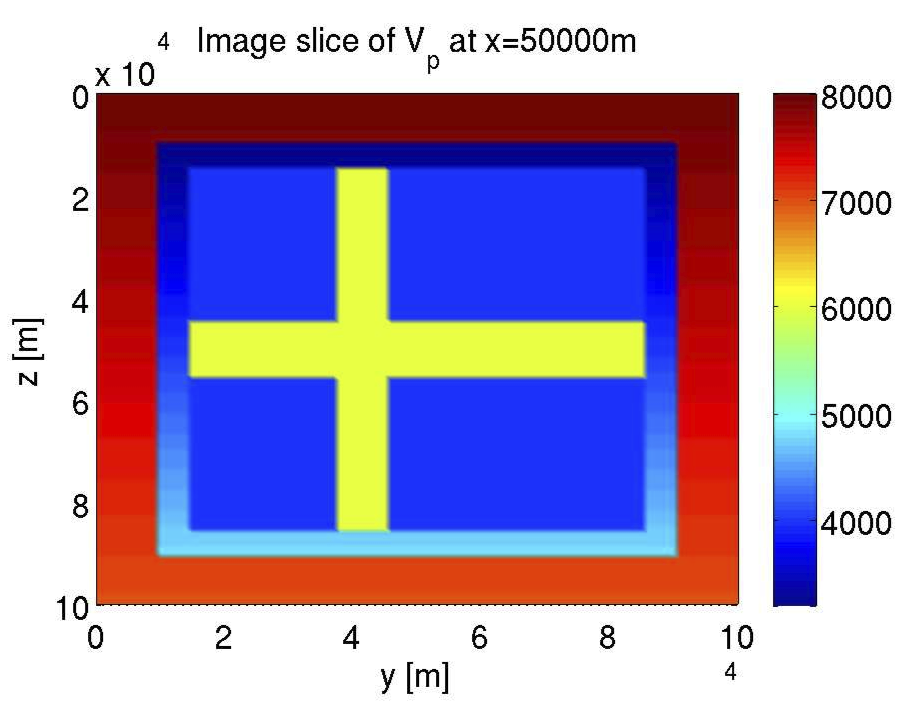
\includegraphics[width=0.45\linewidth]{flag.png}
  \caption{Examples of material models specified with the block command.}
  \label{fig:blockpics}
\end{centering}
\end{figure}
An image of $V_p$ in the plane $x=50,000$ is shown in Figure~\ref{fig:blockpics} (left).

Several block commands can be combined to generate more complicated material models, for example
\begin{verbatim}
block vp=8000 vs=4500 rho=3300 vpgrad=-0.01
block vp=3000 vs=2000 rho=1000 \
      x1=1e4 x2=9e4 y1=1e4 y2=9e4 z1=1e4 z2=9e4 vpgrad=0.02
block vp=4000 vs=2500 rho=2000 \
      x1=15e3 x2=85e3 y1=15e3 y2=85e3 z1=15e3 z2=85e3
block vp=6000 vs=3500 rho=2700 \
      x1=15e3 x2=85e3 y1=15e3 y2=85e3 z1=45e3 z2=55e3
block vp=6000 vs=3500 rho=2700 \
      x1=15e3 x2=85e3 z1=15e3 z2=85e3 y1=38e3 y2=45e3
\end{verbatim}
This material is displayed on the right side of Figure~\ref{fig:blockpics}.

%%%%%%%%%%%%%%%%%%%%%%%%%%%%%%%%%%%%%
\section{The efile command} \label{sec:efile}
%%%%%%%%%%%%%%%%%%%%%%%%%%%%%%%%%%%%%
\begin{figure}
\begin{centering}
  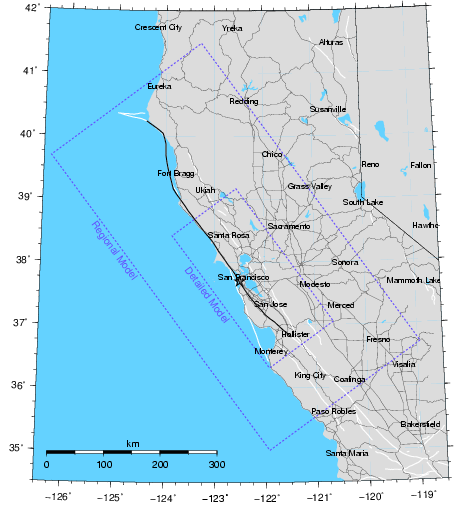
\includegraphics[width=0.49\textwidth]{velmodelbb_roads.png} \hfil
  \caption{The geographical extent of the etree models for Northern California and the San Francisco
  bay area.}
  \label{fig:sfmodel}
\end{centering}
\end{figure}
The efile command is used to obtain material properties from an etree database file. Etree data
bases use an oct-tree data structure, which allows material properties to be represented with finer
spatial resolution near the surface. Topography and bathymetry information is included in the data
base. Note that the same etree database file can be used independently of the grid size. We
currently have access to an etree database file for Northern California and the extended San
Francisco bay area. The geographical extent of the etree model is given in Table~\ref{tab:sfdata},
which also is shown on a map in Figure~\ref{fig:sfmodel}. This model was developed by the USGS and
can currently be downloaded from {\tt http://earthquake.usgs.gov/regional/nca/3Dgeologic}. Be aware
that the files are large (8 + 6 Gbyte) and can take a very long time to download.
\begin{table}
\begin{center}
\begin{tabular}{|l|l|l|} \hline
\multicolumn{3}{|c|}{\bf Detailed Model} \\ \hline
Corner & Longitude & Latitude \\ \hline
SE & -120.64040 & 37.04718 \\ \hline
SW & -121.91833 & 36.31746 \\ \hline
NW & -123.85736 & 38.42426 \\ \hline
NE & -122.56127 & 39.17461 \\ \hline
\end{tabular} \hspace{5 mm}
\begin{tabular}{|l|l|l|} \hline
\multicolumn{3}{|c|}{\bf Regional Model} \\ \hline
Corner & Longitude & Latitude \\ \hline
SE & -118.944514 & 36.702176 \\ \hline
SW & -121.930857 & 35.009018 \\ \hline
NW & -126.353173 & 39.680558 \\ \hline
NE & -123.273199 & 41.48486\\ \hline
\end{tabular}
\caption{Geographical extent (NAD27 projection) for the central California velocity models. Both
  models are defined down to 45 km depth.}\label{tab:sfdata}
\end{center}
\end{table}%

In the etree database, material properties are stored as functions of geographical coordinates
(latitude, longitude, elevation), and \emph{SW4} must determine the geographical coordinates before it
obtains the material properties from the database. Depending on the options of the \verb+grid+
command, \emph{SW4} either uses formulas (\ref{eq:lat})-(\ref{eq:lon}), or the \verb+proj.4+
library, to compute the mapping. Internally to \emph{SW4}, the \emph{cencalvm} software library is
used to query the etree database, which in turn relies on additional libraries. The description in
this section assumes that \emph{SW4} has been configured to use the \verb+efile+ command, see
Section~\ref{cha:installing-sw4} for details.

It is important to note the bounds of the geographical region in the database. Assuming the
computational domain is contained within the bounds of the database, it is easy to set up the
material model in the input file:
\begin{verbatim}
grid x=100e3 y=100e3 z=40e3 lat=38.0 lon=-121.8 az=144 h=1000
efile etree=/p/lscratchd/andersp/USGSBayAreaVM-08.3.0.etree 
\end{verbatim}
To verify that the computational domain is inside the etree database, we recommend checking the
geographical coordinates on a map during the construction of the input file. We often use the Google Earth
program for this purpose.
%
In the case when the computational domain is larger than the region covered by the efile, a block
command can be used to assign material properties to grid points outside of the efile region:
\begin{verbatim}
grid x=300000 y=300000 z=60000 lat=38 lon=-121.5 az=135 nx=100
block vp=8000 vs=4000 rho=1000 rhograd=0.5
efile etree=/p/lscratchd/andersp/USGSBayAreaVM-08.3.0.etree 
\end{verbatim}
However, sharp jumps in material properties can lead to significant scattering of seismic waves. In
some cases, better results can be obtained by reducing the size of the computational domain to match
the extent of the etree region.

To enable use of the extended SF model, the extended etree file must also be downloaded and
then added to the efile command line (file names have been shortened for improved readability):
\begin{verbatim}
efile etree=USGSBayAreaVM.etree xetree=USGSBayAreaVMExt.etree
\end{verbatim}

%%%%%%%%%%%%%%%%%%%%%%%%%%%%%%
\section{The pfile command}\label{sec:pfile}
%%%%%%%%%%%%%%%%%%%%%%%%%%%%%%
The pfile command can be used to assign material properties based on depth profiles. A pfile
contains the values of the model features (P-velocity, S-velocity, density, and optionally the
attenuation factors $Q_P$ and $Q_S$) as function of depth at points on a regular lattice covering
the horizontal extent of the computational domain. The points on the lattice are either defined by
their latitude and longitude coordinates, or by the $x$ and $y$-coordinates. The number of grid
points in the depth direction needs to be the same for all profiles, but the grid spacing does not
need to be uniform and can also be different for each profile. Material discontinuities can be
represented by two material values for the same depth value. Material layers, which only occur in a
subset of the profiles, can be tapered to have zero thickness in the remaining profiles. This is
handled by introducing multiple data points with the same depth and material values in a profile.

The lattice of the pfile does not need to have any relation to the computational mesh used in
\emph{SW4} and is often much coarser. The material properties in the computational mesh are assigned
values using Gaussian averaging between the nearest $N_G\times N_G$ profiles in the
latitude-longitude plane and linear interpolation in the depth direction. Let the grid point have
longitude $\theta$, latitude $\phi$ and depth $d$. Material properties are first linearly
interpolated in the depth direction along each profile and then averaged in the latitude-longitude
plane. The number of points in the Gaussian averaging, $N_G$, is assigned by the user in the
\verb+pfile+ command. For example, the following line in the input file makes \emph{SW4} read a
pfile named \verb+material.ppmod+:
\begin{verbatim}
pfile filename=material.ppmod vsmin=1000 vpmin=1732 smoothingsize=4
\end{verbatim}
The optional \verb+vsmin+ and \verb+vpmin+ keywords are used to assign minimum threshold values for
the $P$- and $S$-velocities, respectively. Here, {\tt smoothingsize=4} means that $N_G=4$ in the
Gaussian averaging. A larger value of $N_G$ ($\geq 5$) is particularily useful to avoid staircasing
imprints when the computational grid is much finer than the pfile lattice, see
Figure~\ref{fig:pfile-smoothing}. The {\tt smoothingsize} keyword can be assigned any number greater
than or equal to one.
\begin{figure}
\begin{centering}
  \includegraphics[width=0.48\textwidth]{ps1.png}\hfill \includegraphics[width=0.48\textwidth]{ps3.png}\\
  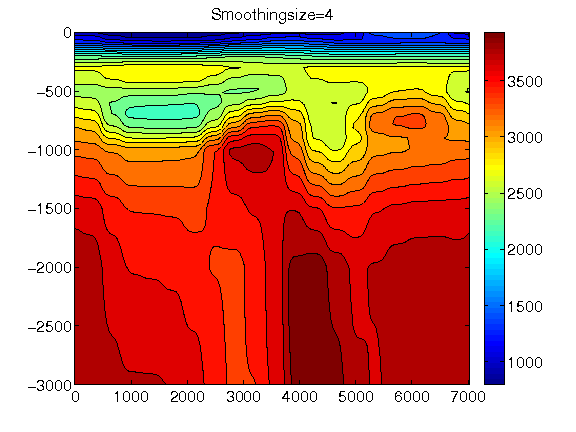
\includegraphics[width=0.48\textwidth]{ps4.png}\hfill 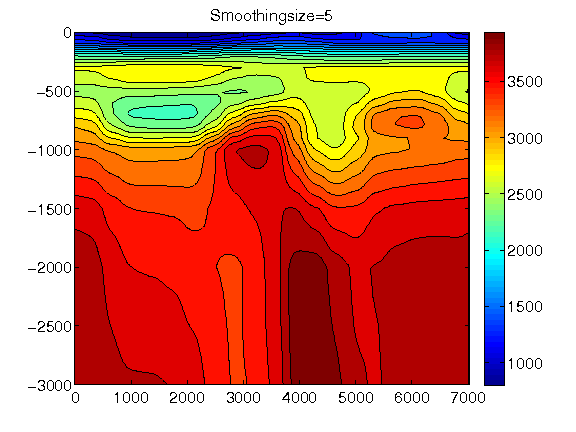
\includegraphics[width=0.48\textwidth]{ps5.png} 
  \caption{The {\tt smoothingsize} parameter can be used to average out imprinting from the
    horizontal lattice in a coarse pfile material model. Here we show $V_P$ in the plane $x=3,500$
    as function of $y$ and $-z$. In this case, {\tt smoothingsize}=1 in the top left, {\tt
    smoothingsize}=3 in the top right, {\tt smoothingsize}=4 in the bottom left, and  {\tt
      smoothingsize}=5 in the bottom right plot.}
  \label{fig:pfile-smoothing}
\end{centering}
\end{figure}

When $N_G$ is odd, the Gaussian averaging starts by finding the closest grid point on the
latitude-longitude lattice, $(\phi_i,\theta_j)$. The material property $c$ ($\rho$, $V_p$, $V_s$,
$Q_s$, or $Q_p$) is assigned by the formula
\begin{equation}\label{eq:gaussian-average}
c(\phi,\theta) = \dfrac{ \sum_{m=i-W}^{i+W} \sum_{n=j-W}^{j+W} c_{m,n} \omega_{m,n} }
{ \sum_{m=i-W}^{i+W} \sum_{n=j-W}^{j+W} \omega_{m,n} },\quad W = \frac{N_G-1}{2},
\end{equation}
where the weights are given by
\[
\omega_{m,n} = e^{-[(\phi_m-\phi)^2 + (\theta_n-\theta)^2]/\alpha^2},\quad \alpha = \frac{N_G \Delta}{2
  \sqrt{-\log 10^{-6}}},
\]
where the parameter $\Delta$ is given in the header of the pfile. It should approximately equal the
grid size in latitude and longitude (which do {\em not} have to be equal). This choice of $\alpha$ makes
the weights $\omega_{m,n}<10^{-6}$ for points that are further from $(\phi_m, \theta_n)$ than $N_G
\Delta/2$, which justifies the truncation of the series in (\ref{eq:gaussian-average}). A
similar procedure is used for even values of $N_G$, but in this case the averaging formula
(\ref{eq:gaussian-average}) is centered around the nearest cell center on the latitude-longitude
lattice.

By default the pfile data are assumed to be given in latitude-longitude coordinates. It is also
possible to read pfiles where the data is given on a Cartesian grid in $(x, y)$-coordinates. To
indicate that the pfile contains data on a  Cartesian grid, use the {\tt style}
option as in the following example:
\begin{verbatim}
pfile filename=materialxy.ppmod vsmin=1000 vpmin=1732 smoothingsize=4 \\
      style=cartesian
\end{verbatim}

Data files for the pfile command are written in an ASCII text format. See
Section~\ref{sec:pfile-format} for a description of both the latitude-longitude pfile and the
Cartesian pfile grid formats.

%%%%%%%%%%%%%%%%%%%%%%%%%%%%%%
\section{The ifile command}\label{sec:ifile}
%%%%%%%%%%%%%%%%%%%%%%%%%%%%%%
The {\bf ifile} command reads a file holding the depth to material interface surfaces. The material
properties between each pair of material surfaces must be defined by the {\bf material} command. The
depth must be non-negative. Zero depth corresponds to the topography. Material surfaces are
specified on a regular lattice in gegraphic coordinates. The unit for depth is meters, while
latitude and longitude are in degrees. The {\bf ifile} command may be combined with other material
specifications and it is {\em not} necessary that the lattice in geographical coordinates covers the
horizontal extent of the computational domain.

Let $N_{mat}\geq 1$ material surfaces be known at longitudes
\[
\phi_i,\quad i=1,2,\ldots,N_{lon},
\]
and latitudes
\[
\theta_j,\quad j=1,2,\ldots,N_{lat},
\]
Note that the latitudes and the longitudes must either be strictly increasing or strictly
decreasing, but the step size may vary. Also note that the lattice points are independent of those
in the {\bf topography} command.

The material surfaces should be given on the regular lattice
\[
d_{q,i,j} = \mbox{depth to surface number $q$ at longitude $\phi_i$, latitude $\theta_j$.}
\]
The material surfaces correspond to material properties in the following way. At longitude $\phi_i$,
latitude $\theta_j$ material number 1 (as defined by the {\bf material} command) occupies depths
$0\leq d \leq d_{1,i,j}$. Material number 2 occupies depths $d_{1,i,j} \leq d \leq d_{2,i,j}$, and
so on. If $d_{1,i,j}=0$, material number 1 is not used. Similarily, material number $k>1$ is not
used if $d_{k-1,i,j} = d_{k,i,j}$. Material properties are only defined for depths down to the last
surface, i.e.,
\[
0\leq d \leq d_{Nmat,i,j}.
\]
If the computational domain extends below the last material surface, it is necessary to use other
commands to define the material properties in those regions.

The material properties can have a constant, linear, quadratic, and square root dependence of
depth. For example, the most general dependence for density is
\[
\rho(d) = \rho_{k,0} + \rho_{k,1} d + \rho_{k,2} d^2 + \rho_{k,1/2} \sqrt{d},\quad d_{k-1,i,j} \leq d < d_{k,i,j}.
\]
Bi-linear interpolation in longitude and latitude is used to define the material surfaces in between
the data points. Note that only constant values are supported for the quality factors
($Q_P$ and $Q_S$) within each material. 

%An example that uses an ifile material description is discussed in Section~\ref{sec:grenoble}. 
The \verb+ifile+ file format is described in Section~\ref{sec:ifile-format}.

%%%%%%%%%%%%%%%%%%%%%%%%%%%%%%
\section{The vimaterial command}\label{sec:vimat}
%%%%%%%%%%%%%%%%%%%%%%%%%%%%%%

The \verb+vimaterial+ command is intended to speed up the reading of large material models for cases
when many simulations use the same computational grid. In order for this command to work, the
\verb+grid+ and \verb+topography+ commands must be identical between runs. An initial run must
construct the material model using the commands described in the previous sections (block, efile,
pfile, ifile). The initial run must also save the material model using the \verb+volimage+
command. Each of these commands saves one scalar property per file, so three files must be saved for
an elastic material. In subsequent simulations the \verb+vimaterial+ command can replace the initial
material model. This approach works the best on machines with a fast (parallel) file system. Also
note that the \verb+volimage+ files can easily become very large, because the material properties
are saved at each grid point.

For example, if the material model and the topography are given in the etree format, the initial run
reads this information and saves it on 5 separate \verb+volimage+ files,
\begin{verbatim}
fileio pfs=1 path=MaterialModel
grid x=275e3 y=120e3 z=40e3 h=400 lon=-122.688 lat=39.009 az=142.25
topography input=efile file=efile/USGSBayAreaVM-08.3.0.etree zmax=8e3 order=3
attenuation nmech=3 phasefreq=1 maxfreq=10

efile query=MAXRES etree=efile/USGSBayAreaVM-08.3.0.etree 

volimage mode=rho file=Lp cycle=0 precision=double
volimage mode=mu file=Lp cycle=0 precision=double
volimage mode=lambda file=Lp cycle=0 precision=double
volimage mode=qp file=Lp cycle=0 precision=double
volimage mode=qs file=Lp cycle=0 precision=double
\end{verbatim}
The \verb+volimage+ files are written in the \verb+MaterialModel+ subdirectory, as specified by the
\verb+path+ option in the \verb+fileio+ command.

Subsequent runs, that use identical grid and topography commands, can read the material
model directly from the \verb+volimage+ files,
\begin{verbatim}
fileio pfs=1 path=OtherRun
grid x=275e3 y=120e3 z=40e3 h=400 lon=-122.688 lat=39.009 az=142.25
topography input=efile file=efile/USGSBayAreaVM-08.3.0.etree zmax=8e3 order=3
attenuation nmech=3 phasefreq=1 maxfreq=10

vimaterial path=MaterialModel rho=Lp.cycle=0.rho.3Dimg mu=Lp.cycle=0.mu.3Dimg \
           lambda=Lp.cycle=0.lambda.3Dimg qs=Lp.cycle=0.qs.3Dimg \
           qp=Lp.cycle=0.qp.3Dimg
\end{verbatim}
Note that a path can be specified in the \verb+vimaterial+ command, and that the \verb+fileio+
command now writes the results to a different directory.

%%%%%%%%%%%%%%%%%%%%%%%%%%%%%%%%%%%%%%%%%%%%%%%%
%\chapter{Mesh refinement} \label{sec:mesh-ref}
%%%%%%%%%%%%%%%%%%%%%%%%%%%%%%%%%%%%%%%%%%%%%%%%

%%%%%%%%%%%%%%%%%%%%%%%%%%%%%%%%%%%%%%%%%%%%%%%%
\chapter{Attenuation}\label{sec:attenuation}
\index{attenuation}
%%%%%%%%%%%%%%%%%%%%%%%%%%%%
\section{Viscoelastic modeling}\label{sec:ve-model}

\emph{SW4} implements a linear viscoelastic material model by superimposing $n$ standard
linear solid (SLS) mechanisms, leading to the governing equations
\begin{equation}\label{eq:ve-wave-eqn}
{\displaystyle \rho\dfrac{\p^2\ub}{\p t^2} = \Lb(\lambda_0,\mu_0)\ub - \sum_{\nu=1}^n
\Lb(\lambda_{\nu},\mu_\nu)\bar{\ub}^{(\nu)} + \Fb,\quad \xb\in\Omega,\ t\geq 0},
\end{equation}
where the spatial operator is
\begin{equation}\label{eq:spatial-op}
\Lb(\lambda,\mu)\ub =: \nabla(\lambda(\nabla\cdot\ub)) + \nabla\cdot \left(2\mu {\cal
  D}(\ub)\right),\quad {\cal D}(\ub) = \frac{1}{2}\left(\nabla \ub + \nabla\ub^T\right).
\end{equation}
The memory variables, $\bar{\ub}^{(\nu)}$, in \eqref{eq:ve-wave-eqn} are governed by the
differential equations
\begin{equation}\label{eq:ve-ode}
\displaystyle \frac{1}{\omega_\nu}\frac{\p \bar{\ub}^{(\nu)}}{\p t} + \bar{\ub}^{(\nu)} = \ub,\quad
\xb\in\Omega,\ t\geq 0,
\end{equation}
for $\nu=1,2,\ldots,n$, where $\omega_\nu>0$ are the relaxation frequencies. For more details on
visco-elastic modeling and the numerical method used by \emph{SW4}, we refer to the paper by
Petersson and Sjogreen~\cite{PetSjo-10b} and the references therein.

There are three components in each of the vector variables $\ub$ and $\bar{\ub}^{(\nu)}$,
$\nu=1,2,\ldots,n$, resulting in $3+3n$ differential equations for as many dependent
variables. Hence, visco-elastic modeling will require more memory and more CPU-time, compared to the
purely elastic case.

The material parameters $\mu_\nu$ and $\lambda_{\nu}$, as well as the relaxation frequencies
$\omega_\nu$ are determined by Emmerich and Korn's~\cite{Emm-Korn-87} least-squares procedure. In
this approach, the material parameters are selected such that the quality factors $Q_S$ and $Q_P$ become close to constant
over a frequency range
\[
\omega_{min}\leq \omega \leq \omega_{max}.
\]
Because the computational cost of viscoelastic modeling increases with the number of mechanisms,
$n$, it is desirable to use the smallest value of $n$ that gives acceptable accuracy in the
approximation of $Q(\omega)$. In Figure~\ref{fig:q2-5}, we present $Q(\omega)$ when the material
coefficients are chosen to approximate $Q=100$ in the frequency band $\omega\in[1,100]$. Clearly,
$n=2$ provides inadequate modeling of a constant $Q$ over two decades in frequency, but $n= 3$ gives
a much better approximation. Increasing $n$ further only leads to small improvements. It is
interesting to note that in all models, $Q(\omega)$ grows rapidly for $\omega>\omega_{max}$. Hence
the viscoelastic model does {\em not} provide significant damping of higher (poorly resolved)
frequencies in the numerical solution, and does {\em not} act as an artificial dissipation.
%-------------------------Figure -------------------------------------
\begin{figure}
\begin{centering}
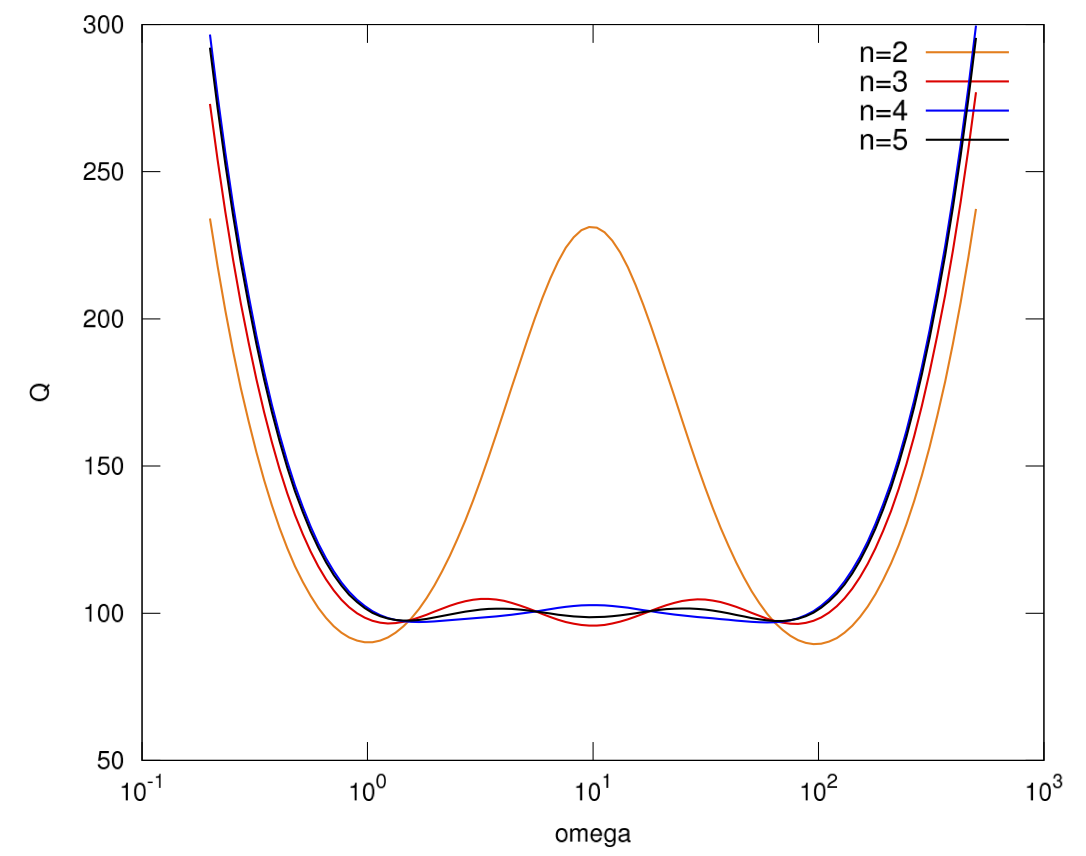
\includegraphics[width=0.7\textwidth]{q2-5.png}
\caption{Actual quality factor $Q(\omega)$ approximating $Q_0=100$ in the frequency band
  $\tilde\omega\in[1,100]$, for different numbers of viscoelastic mechanisms.}
\label{fig:q2-5}
\end{centering}
\end{figure}

Wave propagation in visco-elastic materials is dispersive, i.e., the phase velocity of a wave depends on
its frequency. Figure~\ref{fig:phase-velo} illustrates that the frequency dependence on the phase
velocity becomes more pronounced when $Q$ gets smaller. Also note that the phase velocity grows
approximately linearly on a logarithmic scale in $\omega$, throughout the frequency band
$[\omega_{min},\omega_{max}]$. Outside this band, the phase velocity tends to constant values.
%-------------------------Figure -------------------------------------
\begin{figure}
\begin{centering}
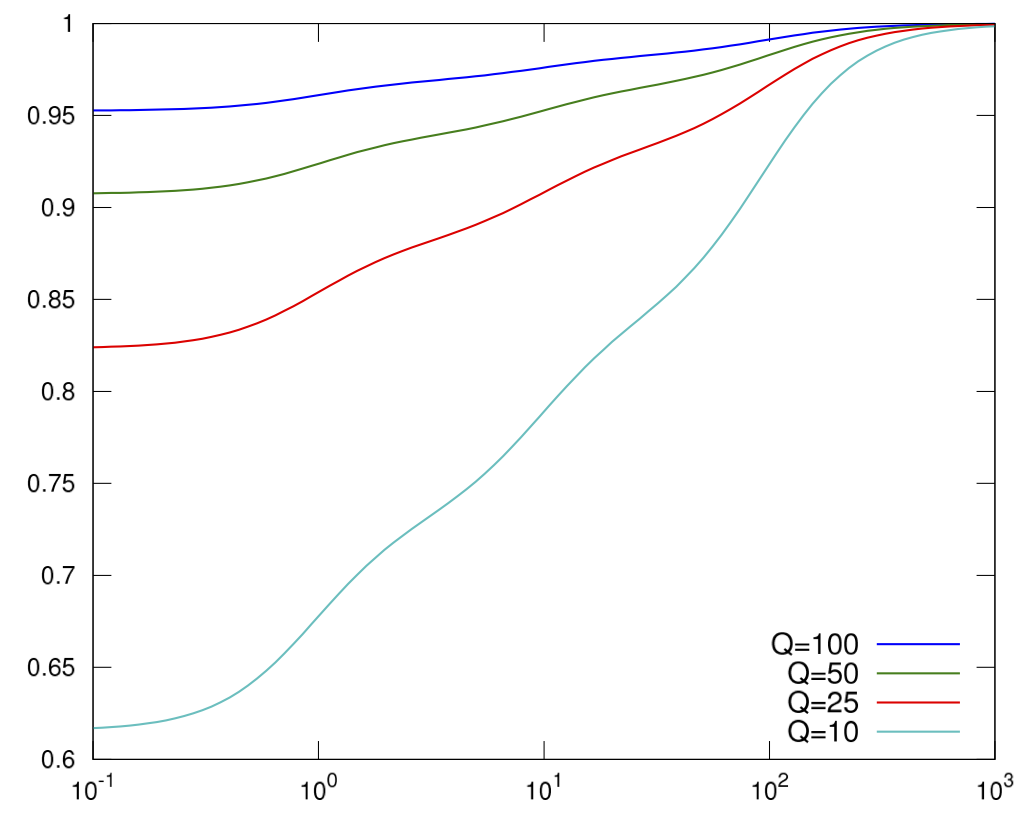
\includegraphics[width=0.7\textwidth]{phase-velo2.png}
\caption{Relative phase velocity over the frequency band
  $\omega\in[1,100]$. Here, $n=3$, and the different colors correspond to different values of $Q$.}
\label{fig:phase-velo}
\end{centering}
\end{figure}
Due to the dispersive nature of visco-elastic materials, it is necessary to specify the reference
frequency, $\omega_r$, at which the phase velocities are specified.

In \emph{SW4}, visco-elastic modeling is enabled by the {\tt attenuation} command. For example, the command
\begin{verbatim}
attenuation nmech=3 phasefreq=2.5 maxfreq=10
\end{verbatim}
enables visco-elastic modeling with three SLS mechanisms, tuned for the max frequency
$f_{max}=10$~Hz, such that the phase velocities are valid at the reference frequency
$f_r=2.5$~Hz. For simplicity, the lower frequency in the modeling is always two orders of
magnitude smaller than the max frequency,
\[
f_{min}=\frac{f_{max}}{100}.
\]

Instead of using \verb+maxfreq+, the upper frequency limit can alternatively be specified through the
\verb+minppw+ option. In this case the material model is first evaluated to find $\min V_S/h$. The
upper frequency limit is then calculated through the relation $P=\min V_s/(h
f)$, i.e.,
\[
f_{max} = \frac{1}{P_{min}}\min \frac{V_s}{h},\quad f_{max} = \mbox{maxfreq},\quad P_{min}=\mbox{minppw}.
\]
The syntax for using \verb+minppw+ is given by
\begin{verbatim}
attenuation nmech=3 phasefreq=2.5 minppw=5
\end{verbatim}

After the input file has been parsed, \emph{SW4} outputs basic information about the attenuation
modeling:
\begin{verbatim}
*** Attenuation parameters calculated for 3 mechanisms, 
      max freq=2.000000e+00 [Hz], min_freq=2.000000e-02 [Hz], \
      velo_freq=1.000000e+00 [Hz]
\end{verbatim}
Note that \verb+max_freq+ = $\omega_{max}/(2\pi)$, etc.
%%%%%%%%%%%%%%%%%%%%%%%%%%%%%%%%%%%%%%%%%%%%%%%%

%%%%%%%%%%%%%%%%%%%%%%%%%%%%%%%%%%%%%%%%%%%%%%%%
\chapter{Output options}
%%%%%%%%%%%%%%%%%%%%%%%%%%%%%%%%%%%%%%%%%%%%%%%%
\section{Setting the output directory}\label{sec:output-dir}
%%%%%%%%%%%%%%%%%%%%%%%%%%%%%%%%%%%%%%%%%
The fileio command is used to specify by which method and in which directory \emph{SW4} should write
its output files.  If the specified directory does not exist, \emph{SW4} attempts to create it for you. The
fileio command may also be used to set the level of diagnostic messages (verbose) and how often the
time step information is printed. For example, the command
\begin{verbatim}
	fileio path=sw4_dir verbose=1 printcycle=10
\end{verbatim}
causes all output files to be written to the directory "./sw4\_dir". The path may be absolute or
relative to the working directory. The \verb+verbose=1+ option enables some extra diagnostic
messages to be printed to standard output. The default value is 0. A higher value gives more
details, but values exceeding 2 give a lot of information and are mostly intended for debugging
purposes. The \verb+printcycle=10+ instructs \emph{SW4} to output time step information every 10
time steps, instead of the default, which is every 1000 time steps.

\paragraph{Serial and Parallel file systems}

Some parallel machines have a dedicated parallel file system that allows many processors to
simultaneously write to the same file. These file systems are often mounted under a particular
sub-directory. By default, \emph{SW4} assumes that the file system is serial, which means that only
one processor is allowed to write to the same file at the same time. If you have access to a
parallel file system, the I/O performance of \emph{SW4} can sometimes be significantly improved by allowing
several processors to simultaneously write to the same file. You enable this feature by using the {\tt pfs=1}
option,
\begin{verbatim}
	fileio pfs=1 nwriters=16 path=/p/lscratcha/my_output_directory
\end{verbatim}
The number of processes (cores) that write to disk can be changed with the \verb+nwriters+
option. By default, \verb+nwriters=8+. The data is buffered on these cores before it is saved to
disk. Increasing \verb+nwriters+ therefore allows larger files to be written using the same amount
or memory. On the other hand, making \verb+nwriters+ smaller usually speeds up the reading or
writing of large files. Note that the parallel file systems is often only accessible from certain
directories. Setting \verb+pfs=1+ without re-directing the output to such a directory may cause
\emph{SW4} to either crash or hang.

%%%%%%%%%%%%%%%%%%%%%%%%%%%%%%%%%%%%%%%%%%%%%%%%%%%%
\section{Time-history at a reciever station: the rec (or sac) command}\label{sec:rec}
%%%%%%%%%%%%%%%%%%%%%%%%%%%%%%%%%%%%%%%%%%%%%%%%%%%%

\emph{SW4} can save the time-history of the solution at a receiver station that is located anywhere
in the computational domain. The basic command looks like this:
\begin{verbatim}
rec x=100e3 y=50e3 z=0 file=sta1
\end{verbatim}
For backwards compatibility with \emph{WPP}, the \verb+rec+ command can also be called \verb+sac+.
The above command makes \emph{SW4} save the three components of the solution at the grid point. The
solution is saved at the grid point which is the closest to the specified $(x,y,z)$ location. 

By default, \emph{SW4} saves the data using the binary Seismic Analysis Code (SAC) format,
see~\cite{Goldstein-et-al}. Since each SAC file contains one component of the solution, the default
\verb+rec+ command results in three files:
\begin{verbatim}
sta1.x  sta1.y  sta1.z
\end{verbatim}
The x,y,z files hold the corresponding solution component. Note that the orientation of the
$z$-component is positive downwards.

The location of the reciever station can alternatively be given in geographical (latitude,
longitude, depth) coordinates. Information about the event location, date, time, and station name is
saved in the header of the SAC file. The event location is taken as the hypocenter, i.e., the
location of the source with the earliest initiation time. The \verb+file+ name is used as the
default station name, but can be modified with the \verb+sta+ option. The date and time are by
default set to be the starting time of the simulation. That datum can be changed by using the
\verb+utcstart+ option in the \verb+time+ command,
%
\begin{verbatim}
time t=10 utcstart=01/04/2012:17:34:45.2343
rec lat=38.25 lon=-122.20 depth=0 file=sta1 sta=EKM
\end{verbatim}
%%
Note that the \verb+depth+ option specifies the depth of the reciever relative to the topography. To
place a reciever at elevation $e$ relative to mean sea level ($e$ is negative below sea level) you
use the option {\tt z=}$-e$. Station that are placed above the topography will be ignored and do not
generate any data.

By default, SAC files are written to disk every 1000 time steps, and at the end of the
simulation. We can change this frequency by using the {\tt writeEvery} option. For example, to
write the SAC file every 100 time steps, you would say
\begin{verbatim}
rec lat=38.25 lon=-122.20 depth=0 file=sta1 writeEvery=100
\end{verbatim}

% {\tt velocity=1} option, \emph{SW4} instead outputs the
%three components of the time-derivative of the solution, i.e., the velocity if \emph{SW4} is setup
%to solve for displacements. The

By default, \emph{SW4} outputs the three components of the solution $\ub(\xb_r,t)=(u_x,u_y,u_z)^T$
at each time step. Here, this quantity is called the displacement. However, it is
important to note that physical meaning of the solution depends on the source time function. For
example, if the displacement corresponds to a \verb+GaussianInt+ source time function, the solution
would hold the corresponding velocity if the time function was changed to a \verb+Gaussian+.

The components that are saved by the \verb+rec+ command can be rotated to the East, North, and vertical
(positive up) directions by using the \verb+nsew+ option,
\begin{verbatim}
rec lat=38.25 lon=-122.20 depth=0 file=sta1 nsew=1
\end{verbatim}
Here, the angle between North and the $x$-axis is determined by the azimuth ({\tt az=...}) option in
the grid command:
\begin{verbatim}
grid x=100e3 y=50e3 z=30e3 lat=37.5 lon=-122.0 az=135
\end{verbatim}
By default, the \verb+rec+ command outputs the three components of the solution (the displacement). The
\verb+rec+ command can also output the time derivative of the solution (the velocity),
\begin{verbatim}
rec lat=38.25 lon=-122.20 depth=0 file=sta1 variables=velocity nsew=1
\end{verbatim}
As indicated here, the \verb+variables+ option can be combined with \verb+nsew+.  To remind the user
of what quantities are saved in a SAC file, we modify the file name extensions according to the
following table:
\begin{center}
%\begin{tabular}{|c|c|c|} \hline
%   & \verb+velocity=0+  & \verb+velocity=1+ \\ \hline
\begin{tabular}{|c|c|c|} \hline
\verb+variables+  & \verb+nsew=0+ & \verb+nsew=1+ \\ \hline\hline
displacement & .x, .y, .z    & .e, .n, .u  \\ \hline
velocity     & .xv, .yv, .zv & .ev, .nv, .uv  \\ \hline
\end{tabular}
\end{center}

It is also possible to save the divergence, curl, or strain of the solution. The {\tt variables}
option governs this behavior. For example,
\begin{verbatim}
rec lat=38.25 lon=-122.20 depth=0 file=sta1 variables=div
\end{verbatim}
outputs a single file named {\tt sta1.div} containing the divergence of the solution, which is
independent of the orientation of the components. Similarly,
\begin{verbatim}
rec lat=38.25 lon=-122.20 depth=0 file=sta1 variables=curl
\end{verbatim}
outputs the Cartesian components of the curl in the files {\tt sta1.curlx}, {\tt sta1.curly}, and
{\tt sta1.curlz}. Furthermore, \emph{SW4} can output the components of the symmetric strain tensor,
\begin{verbatim}
rec lat=38.25 lon=-122.20 depth=0 file=sta1 variables=strains
\end{verbatim}
In this case, six files are generated: {\tt sta1.xx}, {\tt sta1.yy}, {\tt sta1.zz}, {\tt sta1.xy},
{\tt sta1.xz}, and {\tt sta1.yz}.

For the curl and the strain, only \verb+nsew=0+ has been implemented. That is, we always output the
Cartesian components of the curl and strain.

%% The {\tt velocity} and {\tt nsew} options also work together with divergence and curl. Setting {\tt
%%   velocity=1} will output the time derivative of any quantity selected by the {\tt variables}
%% option. The {\tt nsew} option has no effect on the scalar divergence field, but {\tt nsew=1} will
%% make \emph{SW4} output a representation of the curl vector in the East, North, and vertical
%% components.  
%% The file name extensions for the div and curl variables are described in the following
%% table:
%% \begin{center}
%% \begin{tabular}{|c|c|c|c|c|} \hline
%%    & \multicolumn{2}{|c|}{\tt variables=div} & \multicolumn{2}{|c|}{\tt variables=curl} \\ \hline
%%    & \verb+velocity=0+  & \verb+velocity=1+ & \verb+velocity=0+  & \verb+velocity=1+  \\ \hline
%% \verb+nsew=0+ & .div & .vdiv & .curlx, .curly, .curlz & .vcurlx, .vcurly, .vcurlz \\ \hline
%% \verb+nsew=1+ & .div & .vdiv & .curle, .curln, .curlu & .vcurle, .vcurln, .vcurlu \\ \hline
%% \end{tabular}
%% \end{center}

%% When {\tt velocity=1}, the strains of the time derivative of the solution are output on files 
%% named {\tt sta1.vxx}, {\tt sta1.vyy}, etc.
%% There is currently no support for outputting the strains in East, North, and vertical coordinates.

\subsection{The ASCII text format}
\emph{SW4} can also output reciever time-histories on an ASCII text format,
\begin{verbatim}
rec lat=38.25 lon=-122.20 depth=0 file=sta1 sacformat=0 usgsformat=1
\end{verbatim}
The ASCII text file holds all components (usually three, but only one when {\tt
  variables=div}, and six when {\tt variables=strains} ) in a single file named {\tt sta1.txt}. When
the \verb+usgsformat=1+ option is used, the file gets extension .txt independently of the
\verb+nsew+ and \verb+variables+ options.  Instead, the header of the file is modified to reflect
its content. Note that you need to give the \verb+sacformat=0+ option unless you want the solution
to be output in both formats.

\subsection{Notes on the {\tt rec} command}
\begin{itemize}
\item The files are treated in the same way on parallel and serial file systems, because the data
  for each recording station originates from one processor (core) and is always written by that processor only.
\item The binary SAC format is described in Section~\ref{sec:sac-format}.
\item The ASCII text format is very simple and is outlined in its header.
\item The binary SAC files can be read by the SAC program. We also provide a matlab/octave script in
  {\tt tools/readsac.m}.
\item The ASCII text file format can be read by the Matlab/Octave script in {\tt tools/readusgs.m}.
%The ASCII text format was slightly modified with the addition of the strain output option. 
%The Matlab/Octave script {\tt tools/readusgsold.m} can be used to read
%the older version of ASCII text files.
\end{itemize}

%%%%%%%%%%%%%%%%%%%%%%%%%%%%%%%%%%%%%%%%%%%%%%%%%%%%%%%%%%%%%
\section{2-D cross-sectional data: the image command}
%%%%%%%%%%%%%%%%%%%%%%%%%%%%%%%%%%%%%%%%%%%%%%%%%%%%%%%%%%%%%
The image command saves two-dimensional horizontal or vertical cross-sectional data at a specified
time level. It can be used for visualizing the solution, making the images for a movie, or checking
material properties. Each image file contains a scalar field as function of the spatial coordinates
in the cross-sectional plane. The scalar field can be either a component of the solution, a derived
quantity of the solution, a material property, or a grid coordinate, All in all, \emph{SW4} can
output twenty-five different types of images, see Section~\ref{keyword:image} for details.

The cross-sectional plane is specified by a Cartesian coordinate ($x$, $y$, or $z$). The image can
be written at a specific time step or at a specified time. Images can also be output at a fixed
frequency, either specified by a time step interval or a time interval.

For example, the command
\begin{verbatim}
image mode=ux y=500 file=picturefile cycle=1
\end{verbatim}
tells \emph{SW4} to output the $x$-displacement component of the solution along the vertical $y=500$
plane.  The data is written to a file named {\tt picturefile.cycle=1.y=500.ux} after the first time
step ({\tt cycle=1}). The example
\begin{verbatim}
image mode=div x=1000 file=picturefile cycleInterval=100
\end{verbatim}
outputs the divergence of the solution field in the $yz$-plane at the grid surface closest to
$x=1000$. The data is written to the files
\begin{verbatim} 
picturefile.cycle=100.x=1000.div
picturefile.cycle=200.x=1000.div
...
\end{verbatim}
With this setup, one image file is output every 100 time steps.

Note that the divergence of the solution field does not contain shear (S) waves and the
rotation (curl) of the solution field does not contain compressional (P) waves. These
options can therefore be used to distinguish between P- and S-waves in the solution.

The hvelmax and vvelmax modes store the maximum in time of the horizontal and vertical velocity
components, respectively. As these names indicate, it is assumed that the sources in \emph{SW4} are
set up for calculating displacements. The horizontal velocity is defined as $\max(|u^N_t|,|u^E_t|)$,
where $u^N$ and $u^E$ are the displacement components in the North and East directions,
respectively. The vertical velocity is $|w_t|$, where $w$ is the displacement component in the
$z$-direction. For these modes, the cycleInterval or timeInterval options only determine how often
the maxima are written to disk; the actual accumulation of the maximuma is performed after each time
step.

When \emph{SW4} is run in parallel, the data that gets saved on an {\tt image} file originates from
all processors that are intersected by the image plane. For horizontal image planes, this means all
processors. To improve the I/O performance, image data is first communicated to a number of
dedicated image writing processors. By default, 8 processors write each image file to disk (or all
processors if \emph{SW4} is run on fewer than 8). This number can be changed using the {\tt fileio}
command,
\begin{verbatim}
fileio nwriters=4
\end{verbatim}
The above command tells \emph{SW4} to use 4 processors to write each image file. For simulations
which use very large number of grid points and many processors, care must be taken to make sure that enough
memory is available to buffer the image data before it is written to disk.

\paragraph{Notes on the image command:}
\begin{itemize}
\item By default, single precision data is saved. Double precision data can be saved by
  using the {\tt precision=double} option.
\item When topography is used, an image plane along the free surface is specified by the {\tt z=0} option.
\item A {\tt mode=topo z=0} image holds the elevation (negative $z$-coordinate) of the raw
  topography. It can only be written when topography is used.
\item A {\tt mode=grid z=0} image holds the $z$-coordinate (negative elevation) of the grid along
  the free surface, which is the actual shape of the upper surface of the computational domain.
\item When topography or mesh refinement is used, vertical image planes intersect all component
grids in the composite grid. In this case, cross-sectional data from all component grids are stored
on the image file.
\item The images files are written in a binary format, see Section~\ref{sec:image-format} for
  details.
\item We provide matlab/octave scripts for reading image files in the {\tt tools} directory. The
  basic function is called {\tt readimagepatch.m}. A higher level interface is provided by the {\tt
    imageinfo.m} and {\tt plotimage.m} scripts.
\end{itemize}

%%%%%%%%%%%%%%%%%%%%%%%%%%%%%%%%%%%%%%%%%%%%%%%%%%%%%%
\section{Creating a GMT script with the gmt command}\label{sec:gmt}
%%%%%%%%%%%%%%%%%%%%%%%%%%%%%%%%%%%%%%%%%%%%%%%%%%%%%%
The Generic Mapping Toolkit (\emph{GMT})~\cite{WesselSmithGMT} is a suite of image generation
programs for geophysical applications. These programs can be used to make postscript plots like
Figure~\ref{fig:topography-gmt}. In the example shown here, topography information is included as
well as information on the general setup of the simulation. Note that the {\tt gmt} command in
\emph{SW4} causes an ASCII text file to be generated. This file contains a UNIX C-shell script with
commands for the \verb+gmt+ programs, holding general information about the run such as geometric
coordinates of the computational domain as well as locations of sources and recievers. There are
many options for these programs, and they might need to be fine-tuned to suit the needs of a particular
application, see the \emph{GMT} documentation for details. 

To have \emph{SW4} generate a \emph{GMT} shell script file, you give the command
\begin{verbatim}
gmt file=bolinas.gmt
\end{verbatim}
%
\begin{figure}
\begin{center}
\includegraphics[width=0.7\textwidth]{topography-gmt-small.png} 
\caption{Location of the source and stations for the Barnwell simulation. This figure was
  generated using the GMT command, see Section~\protect\ref{keyword:gmt} for details.}
\label{fig:topography-gmt}
\end{center}
\end{figure}
%

%%%%%%%%%%%%%%%%%%%%%%%%%%%%%%%%%%%%%%%%%%%%%%%%
\chapter{Examples (in progress)} \label{sec:examples}
%%%%%%%%%%%%%%%%%%%%%%%%%%%%%%%%%%%%%%%%%%%%%%%%

\section{The elastic layer over half-space problem: LOH.1}
The LOH.1 problem, defined in the input script \verb+examples/scec/LOH.1-h50.in+, has a layered
material model where the top 1000 meters ($z\in [0, 1000m]$) has different properties than the rest of the
domain. The computational domain is taken to be $(x,y,z) \in [0,30000]^2\times [0,17000]$. The
grid size is choosen to be $h=50\,m$ and the material properties in the
different layers are described by
\begin{verbatim}
grid h=50 x=30000 y=30000 z=17000
block vp=4000 vs=2000 rho=2600 
block vp=6000 vs=3464 rho=2700 z1=1000
\end{verbatim}
The problem is driven by a single point moment source, positioned in the lower half-space. The time
function in this problem is a Gaussian (if setup as in the input file, the Gaussian source is
equivalent to using a Brune time function followed by a post processing deconvolution step, as is
described in~\cite{Day-2001}). The advantage of using the Gaussian is that no post processing is
necessary before comparing to the results in~\cite{Day-2001}, and the Gaussian function produces
less high wave number waves which are poorly resolved on the computational mesh. Note that
\verb+freq=16.6667+ corresponds to the spread $\sigma=0.06$ in the Gaussian time function. The lines
to setup the source and the time duration of the simulation are:
\begin{verbatim}
time t=9
source x=15000 y=15000 z=2000 Mxy=1 m0=1e18 t0=0.36 freq=16.6667 \ 
       type=Gaussian
\end{verbatim}

The solution is recorded in an array of receivers: 
\begin{verbatim}
rec x=15600 y=15800 z=0 file=sta01
rec x=16200 y=16600 z=0 file=sta02
rec x=16800 y=17400 z=0 file=sta03
rec x=17400 y=18200 z=0 file=sta04
rec x=18000 y=19000 z=0 file=sta05
rec x=18600 y=19800 z=0 file=sta06
rec x=19200 y=20600 z=0 file=sta07
rec x=19800 y=21400 z=0 file=sta08
rec x=20400 y=22200 z=0 file=sta09
rec x=21000 y=23000 z=0 file=sta10
\end{verbatim}
The velocity time histories for station 10 are shown in Figure~\ref{fig:LOH1} together with a
semi-analytical solution.  We conclude that most features in the solution are very well captured on
the grid with $h=50$, but the solution becomes almost identical with the semi-analytical solution
when the grid is refined to $h=25$. As is customary in seismology, the velocity components have been
rotated to polar componenets, with the origin at the source. The {\tt rec} command outputs the
$u_x$, $u_y$ and $u_z$-components of the velocity. These components are rotated to radial and
transverse components using the transformations,
\[
u_{rad} = 0.6 u_x + 0.8 u_y,\quad u_{tran} = -0.8 u_x + 0.6 u_y.
\]
The vertical component is given by $u_z$ (positive downwards).
\begin{figure}[ht]
  \begin{center}
    \includegraphics[width=0.90\textwidth]{radial-loh1c.png}\\
    \includegraphics[width=0.90\textwidth]{transverse-loh1c.png}\\
    \includegraphics[width=0.90\textwidth]{vertical-loh1c.png}
    \caption{LOH.1: The radial (top), transverse (middle) and vertical (bottom) velocities for
      receiver number 10. Here the numerical solutions are plotted in red ($h=25$) and blue
      ($h=50$), while the semi-analytical solution is plotted in black (almost indistinguishable
      from the red curve).}
    \label{fig:LOH1}
  \end{center}
\end{figure}

By using formulas (\ref{eq:resolutionformula})-(\ref{eq:upper-power-freq}), we can
calculate the number of points per wave length for this simulation. Since we are using a
Gaussian time-function, the center frequency is $f_0=1/(2\pi\sigma)\approx 2.6526$ and we estimate
the highest significant frequency to be $f_{max}\approx 2.5 f_0 = 6.6315$ Hz. The material model has $\min V_s =
2000$ m/s. The coarser grid has size $h=50$ m, which results in
\[
P = \dfrac{2000}{50\cdot 6.6315} \approx 6.03.
\]
From our previous discussion (see Section~\ref{sec:grid-size}), 6 points per wave length is on the low side,
but visual inspection of Figure~\ref{fig:LOH1} indicates very good agreement of the wave forms. The
finer grid with $h=25$ gives $P\approx 12.1$. For the purpose of most practical calculations, we
suggest using in between $P=6$ and $P=12$ grid points per shortest wave length.

\section{The visco-elastic layer over half-space problem: LOH.3}



%%%%%%%%%%%%%%%%%%%%%%%%%%%%%%%%%%%%%%%%%%%%%%%%
\chapter{Keywords in the input file (in progress)}\label{chap:keywords}
%%%%%%%%%%%%%%%%%%%%%%%%%%%%%%%%%%%%%%%%%%%%%%%%
The syntax of the input file is
\begin{verbatim}
command1 parameter1=value1 parameter2=value2 ... parameterN=valueN
# comments are disregarded
command2 parameter1=value1 parameter2=value2 ... parameterM=valueM
...
\end{verbatim}
Each command starts at the beginning of the line and ends at the end of the same line. Blank and
comment lines are disregarded. A comment is a line starting with a \# character. The order of the
parameters within each command makes no difference. The material commands (block, ifile, pfile, and efile)
are applied in the order they appear. The ordering of all other commands is inconsequential. Note
that the entire input file is read before the simulation starts.

Parameter values are either integers (-2,0,5,...), real numbers (20.5, -0.05, 3.4e4), or strings
(earthquake, my-favorite-simulation). Note that there must be no spaces around the = signs and
strings are given without quotation marks and must not contain spaces. Depending on the specific
command, some parameter values are required to fall within specified ranges.

A breif description of all commands is given in the following sections. The commands marked as
[required] must be present in all \emph{SW4} input files, while those marked as [optional] are just
that. Other commands, such as those specifying the material model can be given by a combination of
different commands (block, pfile, efile, or ifile). Note that some required commands must occur
exactly once (grid, time). Some optional commands should not occur more than once (topography,
fileio, prefilter, globalmaterial, gmt, developer). Any number of output commands can
be given (rec, image, volimage). Unless \emph{SW4} is run in one of its test modes (twilight,
testlamb, testpointsource), at least one source must be specified, and the material must be specifed
by at least one of the (block, pfile, ifile, efile) commands. Also note that the test modes are
mutually exclusive. Not all of these rules are currently enforced by the parser, but \emph{SW4} can
give unexpected behavior if they are violated.

Note that the same command parser is used for \emph{SW4} and its companion code \emph{SW4opt}, which
calculates source parameters from seismic observations. Here we only document the commands and options
that are relevant for \emph{SW4}.

%%%%%%%%%%%%%%%%%%%%%%%%%%%%%%%%%%%%%%%%%%%%%%%
\section{Basic commands}
%%%%%%%%%%%%%%%%%%%%%%%%%%%%%%%%%%%%%%%%%%%%%%%

%%%%%%%%%%%%%%%%%%%%%%%%%%%%%%%%%%%%%%%%%%%%%%%
\subsection{fileio [optional]}
\index{command!fileio}
%%%%%%%%%%%%%%%%%%%%%%%%%%%%%%%%%%%%%%%%%%%%%%%
The {\bf fileio} command is used for specifying output directories, setting the amount of
information outputted by \emph{SW4}, the output frequency during the time-stepping, as well
as enabling fast I/O for parallel file system. See \S~\ref{sec:output-dir} for more information.
\begin{flushleft}\bf
Syntax:\\ \tt fileio path=... verbose=... printcycle=... pfs=... nwriters=... \\ 
\bf Required parameters:\\ 
\rm None
\end{flushleft}
\begin{center}
\begin{tabular}{|l|p{8cm}|l|l|} \hline
\multicolumn{4}{|c|}{\bf fileio command parameters}\\ \hline
\bf{Option} & \bf{Description} & \bf{Type} & \bf{Default} \\ \hline \hline
path        & path to a directory where all output will be written & string & . \\ \hline
verbose	    & sets the level of diagnostic messages written to standard out ($\geq 0$) & int & 0  \\ \hline
printcycle  & sets the interval for printing the cycle, time, dt info & int & 100 \\ \hline
pfs         & assume a parallel (1) or serial (0) file system when writing files (several
processes can simultaneously write the same file on a parallel file system) & int & 0 \\ \hline
nwriters    & set the number of processes that write an image or volimage file & int & 8 \\ \hline
\end{tabular}
\end{center}
\index{fileio parameters!path, verbose, printcycle, pfs, nwriters}

%%%%%%%%%%%%%%%%%%%%%%%%%%%%%%%%%%%%%%%%%%%%%%%%%%%%%%%%
\subsection{grid [required]}
\index{command!grid}
\label{keyword:grid}
%%%%%%%%%%%%%%%%%%%%%%%%%%%%%%%%%%%%%%%%%%%%%%%%%%%%%%%%
\begin{flushleft}
\bf Syntax:\\
\tt
grid nx=...  ny=...  nz=...
x=... y=... z=... h=... lat=... lon=... az=... proj=... ellipse=... mlat=... mlon=...\\
\bf Required parameters:\\
\rm See below.
\end{flushleft}
The grid command specifies the extent of the computational domain and the grid size in the base
grid. Optionally the grid command also specifies the latitude and longitude of the origin and the
azimuth angle between North and the $x$-axis. A number of different projections can be specified.
%The ghostpts option is only relevant for testing and should normally never be used.
%When grid refinement is used, the base grid is the coarsest grid. 

There are three basic ways of specifying the extent of the computational domain and the grid size:  
\begin{itemize}
   \item number of grid points in all three directions and the grid size: {\bf nx=... ny=... nz=... h=...}
   \item lenghts in all three directions and the grid size: {\bf x=... y=... z=... h=...}
   \item lenghts in all three directions and the number of grid points in one direction (the
   x-direction in this example): {\bf x=... y=... z=... nx=...}
\end{itemize}
It is not allowed to over-specify the grid size. For example, if {\bf x=...} is given, you can not
specify both {\bf h=...} and {\bf nx=...}. Similarly, it is not allowed to over-specify the extent
of the computational domain. For example, when {\bf h=...} is given, you can not prescribe both {\bf
  y=...} and {\bf ny=...}.
%
\begin{center}
\begin{tabular}{|l|p{8cm}|l|l|l|} \hline
\multicolumn{5}{|c|}{\bf grid command parameters (part 1)}\\ \hline
\bf{Option} & \bf{Description} & \bf{Type} & \bf{Units} & \bf{Default}\\ \hline \hline
x & physical dimension of grid in the x-direction & real & m & none\\ \hline
y & physical dimension of grid in the y-direction & real & m & none\\ \hline
z & physical dimension of grid in the z-direction & real & m & none\\ \hline
\hline
h & grid spacing & real & m & none\\ \hline
\hline
nx & number of grid points in the x-direction & int & none & none\\ \hline
ny & number of grid points in the y-direction & int & none & none\\ \hline	
nz & number of grid points in the z-direction & int & none & none\\ \hline	
\end{tabular}
\end{center}
\index{grid parameters!size - x, y, z, h, nx, ny, nz}

The default projection is spheriodal as described by equations \eqref{eq:lat}-\eqref{eq:lon}. You
can change the parameter $M$ with the {\bf mlat} keyword. By using the {\bf mlon} keyword, you
modify the projection by replacing $M\cos(\phi\pi/180)$ in \eqref{eq:lon} by the constant
$M_{lon}$. More accurate projections are available through the Proj4 library (if \emph{SW4} was
built with Proj4 support). These projections are enabled by using the {\bf proj} and/or {\bf ellps}
keywords. See the Proj4 documentation for details.
\begin{center}
\begin{tabular}{|l|p{8cm}|l|l|l|} \hline
\multicolumn{5}{|c|}{\bf grid command parameters (geographical coordinates and projection)}\\ \hline
\bf{Option} & \bf{Description} & \bf{Type} & \bf{Units} & \bf{Default}\\ \hline \hline
az & clockwise angle from North to the x-axis & real & degrees & 135.0 \\ \hline
lat & latitude geographical coordinate of the origin & real & degrees & 37.0 \\ \hline
lon & longitude geographical coordinate of the origin & real & degrees & -118.0 \\ \hline
mlat & meters per degree of latitude (spheroidal projection) & real & meters & 111,319.5 \\ \hline
mlon & meters per degree of longitude (spheroidal projection) & real & meters & None \\ \hline
proj & name of  projection (see proj4 documentation) & string & None & utm \\ \hline
ellps & name of ellipse (see proj4 documentation) & string & None & WGS84 \\ \hline
\end{tabular}
\end{center}
\index{grid parameters!location - az, lat, lon, proj, ellipse, mlat, mlon}

%%%%%%%%%%%%%%%%%%%%%%%%%%%%%%%%%%%%%%%%%%%%%%%%%%%%%%%%
\subsection{time [required]}
\index{command!time}
%%%%%%%%%%%%%%%%%%%%%%%%%%%%%%%%%%%%%%%%%%%%%%%%%%%%%%%%
\begin{flushleft}
\bf Syntax:\\
\tt
time t=... steps=... utcstart=...\\
\bf Required parameters:\\
\tt t \rm or \tt steps
\end{flushleft}
The time command specifies the duration of the simulation. You can either specify the final time in
seconds by using {\bf t}, or specify the number of time-steps with {\bf steps}.  The size of the
time step is computed internally by \emph{SW4}. You may not over specify the duration of the
simulation, i.e., you can not give both {\bf t=...} and {\bf steps=...}.

The optional {\bf utcstart} keyword is used to assign the Universal Time Coordinate (UTC)
corresponding to simulation time $t=0$. The format of the UTC time is a string (without quotation)
``month/day/year:hour:minute:second.millisecond''. For example, the 17th hour, 34th minute, 12th
second and 233th millisecond of January 31, year 2012, is encoded as {\bf
  utcstart=01/31/2012:17:34:12.233}. When the UTC time is set, all time-series (saved with the {\tt
  rec} command) are time stamped with that datum. The UTC time stamp is essential for correctly
aligning observed data when solving the inverse problem with \emph{SW4opt}.

Note that the \verb+prefilter+ command does {\it not} modify the start time. This is a change from
\emph{WPP}. See \S\ref{keyword:prefilter} for a discussion.
%
\begin{center}
\begin{tabular}{|l|p{8cm}|l|l|l|} \hline
\multicolumn{5}{|c|}{\bf time command parameters}\\ \hline
{\bf Option} & {\bf Description} & {\bf Type} & {\bf Units} & {\bf Default} \\ \hline \hline
t & duration of simulation & real & s	& none \\ \hline
steps & number of cycles (time-steps) to advance & int & none & none\\ \hline
utcstart & month/day/year:hour:minute:second.millisecond & string & datum & none\\ \hline
\end{tabular}
\end{center}
\index{time parameters!t, steps}

%%%%%%%%%%%%%%%%%%%%%%%%%%%%%%%%%%%%%%%%%%%%%%%%%%%
\subsection{supergrid [optional]} \label{sec:supergrid}
\index{command!supergrid}
\label{keyword:supergrid}
%%%%%%%%%%%%%%%%%%%%%%%%%%%%%%%%%%%%%%%%%%%%%%%%%%%
\begin{flushleft}\bf
Syntax:\\
\tt
supergrid gp=... dc=...
\\
\bf Required parameters:\\
\rm
None
\end{flushleft}
Note that the keywords are different from \emph{WPP}. Also note that
increasing {\tt dc} may lead to instabilities.
\begin{center}
\begin{tabular}{|l|p{10cm}|l|l|} \hline
\multicolumn{4}{|c|}{\bf supergrid command parameters}\\ \hline
\bf{Option} & \bf{Description} & \bf{Type} & \bf{Default} \\ \hline \hline
%
gp &  Number of grid points in the supergrid layer & int & 30\\ \hline
%
dc & Damping coefficient in supergrid region & real & 0.04 \\ \hline
\end{tabular}
\end{center}
\index{supergrid parameters!thickness, damping}

%%%%%%%%%%%%%%%%%%%%%%%%%%%%%%%%%%%%%%%%%%%%%%%
\subsection{prefilter [optional]}\label{keyword:prefilter}
\index{command!prefilter}
%%%%%%%%%%%%%%%%%%%%%%%%%%%%%%%%%%%%%%%%%%%%%%%
\begin{flushleft}
\bf
Syntax:\\
\tt prefilter fc1=... fc2=... type=... passes=... order=...\\
\bf 
Required parameters:\\
\rm 
None
\end{flushleft}
The \verb+prefilter+ command is used to filter all source time functions before the simulation
starts. This approach gives the same result as filtering all time-series after the simulation is
completed. Hence, the \verb+prefilter+ command can be used to reduce the amount of post
processing. The command is particularly useful in combination with the {\bf Dirac} source time
function, which triggers all frequencies on the grid. The \verb+prefilter+ option is also useful for
removing unphysical modes from image files, e.g. max velocities or displacements.  The
\verb+prefilter+ command modifies the time functions in all source commands using a discrete
Butterworth filter. Lowpass and bandpass filters are supported, with orders between 1 and 10. Only
the {\bf fc2} frequency is used for lowpass filters, while it is assumed that {\bf fc1}$<${\bf fc2}
for bandpass filters. The filtering is either forwards in time ({\bf passes=1}), or forwards and
backwards ({\bf passes=2}). For {\bf passes=1}, the filter is causual but gives the filtered signal
a phase shift. When {\bf passes=2} the filter has zero phase shift, but is acausual. In this case,
the filtered signal is only exponentially small as $t\to-\infty$. In order to avoid unphysical
oscillations due to an abrupt start, an estimate of the length of this tail is calculated. A warning
message is printed to stdout if the time shift ({\bf t0}) in the source is smaller than this value.
\begin{center}
\begin{tabular}{|l|p{8cm}|l|l|l|} \hline
\multicolumn{5}{|c|}{\bf prefilter command parameters}\\ \hline
\bf{Option} & \bf{Description} & \bf{Type} & \bf{Units} & \bf{Default} \\ 
\hline \hline
fc1 & first (low) corner frequency in the filter $(>0)$   & real  & Hz & 0.1 \\ \hline
fc2 & second (high) corner frequency in the filter $(>0)$ & real  & Hz & 1.0 \\ \hline
type & lowpass or bandpass                                & string & None & bandpass \\ \hline
passes & number of passes (1 or 2) & int & None & 2 \\ \hline
order  & order of filter (1-10) & int & None & 2 \\ \hline
\end{tabular}
\end{center}
\index{prefilter parameters!fc1, maxfreq}

%%%%%%%%%%%%%%%%%%%%%%%%%%%%%%%%%%%%%%%%%%%%%%%%%%%%%%%%
\section{Sources [required]}
%%%%%%%%%%%%%%%%%%%%%%%%%%%%%%%%%%%%%%%%%%%%%%%%%%%%%%%%

%%%%%%%%%%%%%%%%%%%%%%%%%%%%%%%%%%%%%%%%%%%%%%%%%%%%%%%%
\subsection{source}
\index{command!source}
\label{keyword:source}
%%%%%%%%%%%%%%%%%%%%%%%%%%%%%%%%%%%%%%%%%%%%%%%%%%%%%%%%
\begin{flushleft}
\bf
Syntax:\\ \tt source
x=... y=... z=... lat=... lon=... depth=... topodepth=... m0=... mxx=... mxy=... mxz=...
myy=... myz=... mzz=... f0=... fx=... fy=... fz=... rake=... strike=... dip=... t0=... 
freq=... type=... ncyc=... dfile=...\\ 
\bf
Required parameters:\\ \rm See below.
\end{flushleft}
There can be multiple source commands in an input file. Each source command either sets up a point
force or a point moment tensor source and should follow the following rules:
\begin{itemize}
\item The location of the source must be specified by either Cartesian ({\bf x, y, z}) or
  geographical ({\bf lat, lon, depth} or {\bf topodepth}) coordinates. The depth below mean sealevel
  ($z=0$) is specified with {\bf z}, while {\bf depth} or {\bf topodepth} specifies the depth below the
  topography.
\item Select a point force or a point moment tensor source:
  \begin{itemize}
  \item Point force: give at least one component of the force vector ({\bf fx, fy, fz}) and
    optionally the amplitude {\bf f0}.
  \item A point moment tensor source can be specified in one of two ways:
    \begin{enumerate}
    \item Seismic moment {\bf m0}, and double couple focal mechanism, {\bf strike/dip/rake} angles
      (as defined in Aki and Richards~\cite{Aki-Richards-02}). 
    \item At least one component of the moment tensor ({\bf mxx}, {\bf mxy}, etc.) and optionally a
      scaling factor {\bf m0}. 
    \end{enumerate}
  \end{itemize}
\item Specify a pre-defined source time function (with the {\bf type} keyword), or give the file
  name for a discrete time function (using the {\bf dfile} keyword).
\end{itemize}
Note that all pre-defined time functions use the {\bf t0} keyword, and all functions except {\bf
  Dirac} also use the {\bf freq} keyword. The only pre-defined time function that uses the {\bf
  ncyc} keyword is {\bf GaussianWindow}.
%
\begin{center}
\begin{tabular}{|l|p{8cm}|l|l|l|} \hline
\multicolumn{5}{|c|}{\bf source command parameters (part 1)}\\ \hline
\bf{Option} & \bf{Description} & \bf{Type} & \bf{Units} & \bf{Default} \\ \hline \hline
x & x position of the source (within domain) & real & m & none \\ \hline
y & y position of the source (within domain) & real & m & none \\ \hline
z & z position of the source (within domain) & real & m & none \\ \hline
\hline
depth & depth of the source $(\geq 0)$ & real & m & none \\ \hline
topodepth & (same as depth) & real & m & none \\ \hline
lat & latitude geographical coordinate of the source & real & degrees & none \\ \hline
lon & longitude geographical coordinate of the source & real & degrees & none \\ \hline
\hline
t0 & offset in time $(\geq 0)$ & real & s & 0.0 \\ \hline
freq & frequency $(>0)$ (not used for Dirac)& real & Hz or rad/s & 1.0 \\ \hline
type & Name of source time function & string & none & RickerInt \\ \hline
ncyc & Number of cycles (must be specified for the GaussianWindow function) & int & none & 0
\\ \hline
dfile & File name for discrete time function & string & none & none \\ \hline
\end{tabular}
\end{center}
\index{source parameters!location - x, y, z, depth, topodepth, lat, lon} \index{source
  parameters!t0, freq, type} The {\bf type} keyword specifies the source time function. It can have
the following values: {\tt GaussianInt, Erf, Gaussian, RickerInt, Ricker, Ramp, Triangle, Sawtooth,
  Smoothwave, VerySmoothBump, Brune, BruneSmoothed, GaussianWindow, Liu, Dirac}, and {\tt
  C6SmoothBump}. The functions are described in \S~\ref{sec:predefined}.  
\index{source time function!GaussianInt, Gaussian, RickerInt, Ricker, Ramp, Triangle, Sawtooth, Smoothwave,
  VerySmoothBump, Brune, BruneSmoothed, GaussianWindow, Liu, Dirac, C6SmoothBump}
\begin{center}
\begin{tabular}{|l|p{8cm}|l|l|l|} \hline
\multicolumn{5}{|c|}{\bf source command parameters (point moment tensor)}\\ \hline
\bf{Option} & \bf{Description} & \bf{Type} & \bf{Units} & \bf{Default} \\ \hline \hline
m0 & moment amplitude & real & Nm & 1.0 \\ \hline
mxx & xx-component of the moment tensor & real & Nm & 0.0 \\ \hline
myy & yy-component of the moment tensor & real & Nm & 0.0 \\ \hline
mzz & zz-component of the moment tensor & real & Nm & 0.0 \\ \hline
mxy & xy-component of the moment tensor & real & Nm & 0.0 \\ \hline
mxz & xz-component of the moment tensor & real & Nm & 0.0 \\ \hline
myz & yz-component of the moment tensor & real & Nm & 0.0 \\ \hline
\hline
strike & strike angle (see Aki and Richards) & real & degrees & none \\ \hline
dip    & dip angle    & real & degrees & none \\ \hline
rake   & rake angle   & real & degrees & none \\ \hline
\end{tabular}
\end{center}
\index{source parameters!moment - m0, mxx, myy, mzz, mxy, mxz, myz}
\index{source parameters!Aki and Richards - strike, dip, rake}
\begin{center}
\begin{tabular}{|l|p{8cm}|l|l|l|} \hline
\multicolumn{5}{|c|}{\bf source command parameters (point force)}\\ \hline
\bf{Option} & \bf{Description} & \bf{Type} & \bf{Units} & \bf{Default} \\ \hline \hline
f0 & point force amplitude & real & N & 1.0 \\ \hline
fx & forcing function in the x direction & real & N & 0.0 \\ \hline
fy & forcing function in the y direction & real & N & 0.0 \\ \hline
fz & forcing function in the z direction & real & N & 0.0 \\ \hline
\end{tabular}
\end{center}
\index{source parameters!point force - f0, fx, fy, fz}

%%%%%%%%%%%%%%%%%%%%%%%%%%%%%%%%%%%%%%%%%%%%%%%%%%%%%%%%
\subsection{rupture}
\index{command!rupture}
\label{keyword:rupture}
%%%%%%%%%%%%%%%%%%%%%%%%%%%%%%%%%%%%%%%%%%%%%%%%%%%%%%%%

%%%%%%%%%%%%%%%%%%%%%%%%%%%%%%%%%%%%%%%%%%%%%%%%%%%%%%%%
\section{The material model [required]} 
%%%%%%%%%%%%%%%%%%%%%%%%%%%%%%%%%%%%%%%%%%%%%%%%%%%%%%%%

It is required that the material model is defined in the entire computational domain. The material
properies are extrapolated to the ghost points if they are not covered by the material model (this
is a change from \emph{WPP}). The material commands \verb+block+, \verb+ifile+, \verb+efile+, and
\verb+pfile+, are applied in the same order as they are given. Hence, it is possible to overwrite
the properties specified by a material command given earlier in the file. This can be particularily
useful when using the \verb+block+ command. Finally, the properties of the optional
\verb+globalmaterial+ command are enforced after all other material commands have been applied. Also
note that the input file is scanned for the \verb+attenuation+ command before any other commands are
parsed. This command may be located anywhere in the input file.

\subsection{attenuation [optional]}
\index{command!attenuation}
\label{keyword:attenuation}
%%%%%%%%%%%%%%%%%%%%%%%%%%%%%%%%%%

The \verb+attenuation+ command is used to enable visco-elastic modeling as described in
Section~\ref{sec:attenuation}. The visco-elastic model is defined through the quality factors $Q_p$
and $Q_s$. Similar to the elastic properties, the quality factors may vary from point to point
throughout the computational domain. If visco-elastic modeling is enabled, the $Q_P$ and $Q_S$
factors must be specified as part of every material command described below. When visco-elastic
modeling is {\em not} enabled, the $Q_P$ and $Q_S$ factors are not required in the material
commands, and are ignored if present.
\begin{flushleft}\bf
Syntax:\\
\tt
attenuation phasefreq=... nmech=... maxfreq=... minppw=...
\\
\bf Required parameters:\\
\rm None \\
\bf Note: \rm you may not specify both \verb+maxfreq+ and \verb+minppw+.
\end{flushleft}
%
\begin{center}
\begin{tabular}{|l|p{8cm}|l|l|l|} \hline
\multicolumn{5}{|c|}{\bf attenuation command parameters}\\ \hline
\bf{Option} & \bf{Description} & \bf{Type} & \bf{Unit} & \bf{Default} \\ \hline \hline
phasefreq & The frequency ($>0$) at which $C_S$ and $C_P$ are specified & real & Hz & 1.0\\ \hline
nmech     & Number of SLS mechanisms to approximate constant $Q_P$ and $Q_S$ (between 1 and 8) & int & None & 3\\ \hline
maxfreq   & The upper frequency limit  ($>0$) for approximating constant $Q_P$ and $Q_S$ & real & Hz & 2.0 \\ \hline
minppw    & Calculate the upper frequency limit based on this number of grid points per shortest
wave length ($>0$)& real & None & None \\ \hline
\end{tabular}
\end{center}
If you specify the \verb+minppw+ option, the upper frequency limit is calculated based on the
relation $P=\min C_s/(h f)$, i.e.,
\[
f_{max} = \frac{1}{P_{min}}\min \frac{C_s}{h},\quad f_{max} = \mbox{maxfreq},\quad P_{min}=\mbox{minppw}.
\]

%%%%%%%%%%%%%%%%%%%%%%%%%%%%%%%%%%%%%%%%%%
\subsection{block}
\index{command!block}
%%%%%%%%%%%%%%%%%%%%%%%%%%%%%%%%%%%%%%%%%%
\label{keyword:block}
\begin{flushleft}\bf
Syntax:\\
\tt block
vp=... vs=... rho=... qp=... qs=... vpgrad=... vsgrad=... rhograd=... absdepth=... x1=... x2=... y1=... y2=... z1=... z2=...\\
\bf
Required parameters:\\
\tt
%vp, vs, rho
vp, vs, rho  (qp and qs with attenuation)
\end{flushleft}
%
The block command specifies material properties that are constant or vary linearly with depth. By
default, the material properties apply to the entire computational domain. By using the optional
parameters {\bf x1=...}, {\bf x2=...}, etc., the material properties are only assigned in parts of
the computational domain. When used together with the {\bf topography} command, the {\bf absdepth}
flag determines how the $z$-coordinates are used. If {\bf absdepth}=0 (default) {\bf z1=...} and
{\bf z2=...} specify depths below the free surface. If {\bf absdepth}=1,  {\bf z1=...} and
{\bf z2=...} bound the $z$-coordinate of the material block.

The gradient parameters {\bf vpgrad}, {\bf vsgrad}, and {\bf rhograd} specify linear variations in the
$z$-direction (downward). The units for {\bf vpgrad} and {\bf vsgrad} are 1/seconds, which
can be interpreted as m/s per m, or km/s per km. The linear variation is relative to the properties at
the free surface ($z=0$ or depth=0 with topography), e.g.,
\[
C_p(z) = {\bf vp} + z \, {\bf vpgrad}.
\]
Note that when {\bf vpgrad} is specified together with ${\bf z1}=z_1$, $C_p(z_1) = {\bf vp} + z_1\,
{\bf vpgrad}$. Hence, the material properties at the top of the block ($z=z_1$) can be very
different from {\bf vp} when $z_1\, {\bf vpgrad}$ is large.
\begin{center}
\begin{tabular}{|l|p{8cm}|l|l|l|} \hline
\multicolumn{5}{|c|}{\bf block command parameters (part 1)}\\ \hline
{\bf Option} & {\bf Description}          & {\bf Type} & {\bf Units} & {\bf Default} \\ \hline 
\hline
vp          & P-wave velocity           & real     & m/s      & none \\ \hline
vs          & S-wave velocity           & real     & m/s      & none \\ \hline
rho         & density                   & real     & kg/m$^3$ & none \\ \hline
%qp or Qp    & P-wave quality factor     & real     & none     & none \\ \hline
%qs or Qs    & S-wave quality factor     & real     & none     & none \\ \hline
vpgrad      & vertical gradient for vp  & real     & s$^{-1}$  & none \\ \hline
vsgrad      & vertical gradient for vs  & real     & s$^{-1}$  & none \\ \hline
rhograd     & vertical gradient for rho & real     & kg/m$^4$  & none \\ \hline
%qp          & P-wave quality factor     & real     & none \\ \hline
%qs          & S-wave quality factor     & real     & none \\ \hline
\end{tabular}
\end{center}
\index{block parameters!vp, vs, rho, vpgrad, vsgrad, rhograd}
%
\begin{center}
\begin{tabular}{|l|p{8cm}|l|l|l|} \hline
\multicolumn{5}{|c|}{\bf block command parameters (part 2)}\\ \hline
{\bf Option} & {\bf Description}          & {\bf Type} & {\bf Units} & {\bf Default} \\ \hline 
\hline
x1          & minimum x-dim for the box shaped sub-region & real & m & -max x \\ \hline
x2          & maximum x-dim for the box shaped sub-region & real & m & 2 max x \\ \hline
\hline
y1          & minimum y-dim for the box shaped sub-region & real & m & -max y \\ \hline
y2          & maximum y-dim for the box shaped sub-region & real & m & 2 max y \\ \hline
\hline
z1          & minimum z-dim for the box shaped sub-region & real & m & -max z \\ \hline
z2          & maximum z-dim for the box shaped sub-region & real & m & 2 max z \\ \hline
\hline
absdepth    & {\tt z1} and {\tt z2} relative to topography (0), or absolute $z$-coordinate (1) & int
& none & 0 \\ \hline 
\end{tabular}
\end{center}
\index{block parameters!x1, x2, y1, y2, z1, z2, absdepth}
%

%%%%%%%%%%%%%%%%%%%%%%%%%%%%%%%%%%%%%%%%%%%%%%%%%%%%%%%%
%  Efiles
%%%%%%%%%%%%%%%%%%%%%%%%%%%%%%%%%%%%%%%%%%%%%%%%%%%%%%%%
\subsection{efile}
\index{command!efile}
\label{keyword:efile}
%%%%%%%%%%%%%%%%%%%%%%%%%%%%%%%%%%%%%%%%%%%%%%%%%%%%%%%%
\begin{flushleft}
\bf
Syntax:\\
\tt
efile etree=... xetree=... logfile=... query=... access=... resolution=...\\
\bf 
Required parameters:\\
\tt etree
\end{flushleft}
\begin{center}
\begin{tabular}{|l|p{8cm}|l|l|l|} \hline
\multicolumn{5}{|c|}{\bf efile command parameters (part 1)}\\ \hline
\bf{Option} & \bf{Description}                                    & \bf{Type} & \bf{Units} & \bf{Default} \\ \hline 
\hline
etree      & full path to the etree database file                 & string   & none   & none \\ \hline
xetree     & full path to the extended etree database file        & string   & none   & none \\ \hline
logfile    & name of log file                                     & string   & none   & none \\ \hline
\end{tabular}
\end{center}
\begin{center}
\begin{tabular}{|l|p{8cm}|l|l|l|} \hline
\multicolumn{5}{|c|}{\bf efile command parameters (part 2)}\\ \hline
\bf{Option} & \bf{Description}                                & \bf{Type} & \bf{Units} & \bf{Default} \\ \hline 
\hline
query      & type of query to perform                         & string  & none   & MAXRES \\ \hline
resolution & average properties over this distance (for query=FIXEDRES) & real  & m      & $h$ \\ \hline
access     & can be set to parallel or serial                 & string  & none   &  parallel \\ \hline
\end{tabular}
\end{center}
\index{efile parameters!logfile, query, resolution, access, etree, xetree}
%
The query option can be set to one of the following:
%
\begin{center}
\begin{tabular}{lp{12cm}} \hline
\bf{query option} & \bf{Description} 
\\ \hline 
MAXRES & Sample the data at the maximum available
resolution in the database. This is the default query type. 
\\ 
FIXEDRES & Average the material properties at the requested resolution, which is specified with the
\verb+resolution+ keyword. The default resolution is the grid spacing. $h$ \\
\end{tabular}
\end{center}
%
For example, to set the data to be sampled at 1 km resolution:
\begin{verbatim}
efile query=FIXEDRES resolution=1000 etree=USGS-SF1906.etree
\end{verbatim}
Note: the logfile option can be used to track if any grid points were outside the etree database
domain, or if any grid points were located in the air.

%
\subsection{pfile}
\index{command!pfile}
\label{keyword:pfile}
%%%%%%%%%%%%%%%%%%%%%%%%%%%%%%%%%%%%%%%%%%%%%%%%%%%%%%%%
\begin{flushleft}\bf
Syntax:\\
\tt
pfile filename=... directory=... smoothingsize=... vpmin=... vsmin=... rhomin=... flatten=... style=... \\
\bf Required parameters:\\
\tt filename
\end{flushleft}
%
\begin{center}
\begin{tabular}{|l|p{8cm}|l|l||l|} \hline
\multicolumn{5}{|c|}{\bf pfile command parameters}\\ \hline
{\bf Option} & {\bf Description}                        & {\bf Type} & {\bf Units} & {\bf Default} \\ \hline 
\hline
filename      & name of input pfile                     & string  & none & none \\ \hline
directory     & name of directory for the input pfile   & string  & none & . \\ \hline
smoothingsize & smooth data over stencil of this width ($\geq 1$) & int & none & 5 \\ \hline
vpmin         & minimum threshold value for $C_p$       & real    & m/s  & 0  \\ \hline
vsmin         & minimum threshold value for $C_s$       & real    & m/s  & 0  \\ \hline
rhomin        & minimum threshold value for density     & real    & m/s  & 0  \\ \hline
flatten       & Flatten the earth model (T or F)        & string  & none & F  \\ \hline
style         & type of grid data: {\tt geographic} or {\tt cartesian} & string  & none & geographic \\ \hline
\end{tabular}
\end{center}

\index{pfile parameters!filename, directory, smoothingsize, vpmin, vsmin, rhomin, flatten, style}

\subsection{ifile}
\index{command!ifile}
\label{keyword:ifile}
%%%%%%%%%%%%%%%%%%%%%%%%%%%%%%%%%%%%%%%%%%%%%%%%%%%%%%%%
\begin{flushleft}\bf
Syntax:\\
\tt ifile filename=... input=...\\
\bf Required parameters:\\
\tt filename
\end{flushleft}
The ifile command specifies the depth of material surfaces as function of longitude and latitude,
and must be used in conjunction with the {\bf material} command. The file format is
described in Section~\ref{sec:ifile-format}.
\begin{center}
\begin{tabular}{|l|p{8cm}|l|l|} \hline
\multicolumn{4}{|c|}{\bf ifile command parameters}\\ \hline
\bf{Option} & \bf{Description} & \bf{Type} & \bf{Default} \\ \hline \hline
filename & name of input file holding material surfaces & string & None  \\ \hline
input & {\tt cartesian} or {\tt geographic} & string & None  \\ \hline
\end{tabular}
\end{center}
\index{ifile parameters!filename}
If {\tt input=cartesian}, the file is assumed to give the material surfaces as function of the $x$-
and $y$-coordinates. If {\tt input=geographic}, they are functions of latitude and longitude. See
Section~\ref{sec:ifile-format} for details.
\subsection{material}
\index{command!material}
\label{keyword:material}
%%%%%%%%%%%%%%%%%%%%%%%%%%%%%%%%%%%%%%%%%%%%%%%%%%%%%%%%
\begin{flushleft}\bf
Syntax:\\
\tt material
id=... vp=... vs=... rho=... vpgrad=... vsgrad=... rhograd=... vp2=... vs2=... rho2=... vpsqrt=... vssqrt=... rhosqrt=...\\ 
\bf Required parameters:\\
\tt id, vp, vs, rho
\end{flushleft}
The {\bf material} command is used to define material properties together with the {\bf ifile}
command, see Section~\ref{sec:ifile-format} for the file format.
\begin{center}
\begin{tabular}{|l|p{8cm}|l|l|} \hline
\multicolumn{4}{|c|}{\bf material command parameters (constants)}\\ \hline
\bf{Option} & \bf{Description} & \bf{Type} & \bf{Default} \\ \hline \hline
id & material ID number $>0$         & int & None  \\ \hline
vp & P-wave velocity & real & None \\ \hline
vs & S-wave velocity & real & None \\ \hline
rho & Density & real & None \\ \hline
%qp or Qp & P-wave quality factor & None & None \\ \hline
%qs or Qs & S-wave quality factor & None & None \\ \hline
\end{tabular}
\end{center}
\index{material parameters!id, vp, vs, rho, qp, qs}
\begin{center}
\begin{tabular}{|l|p{8cm}|l|l|} \hline
\multicolumn{4}{|c|}{\bf material command parameters (gradients)}\\ \hline
\bf{Option} & \bf{Description} & \bf{Type} & \bf{Default} \\ \hline \hline
vpgrad & P-velocity gradient & real & 0.0 \\ \hline
vsgrad & S-velocity gradient & real & 0.0 \\ \hline
rhograd & Density gradient   & real & 0.0 \\ \hline
\end{tabular}
\end{center}
\index{material parameters!vpgrad, vsgrad, rhograd}
\begin{center}
\begin{tabular}{|l|p{8cm}|l|l|} \hline
\multicolumn{4}{|c|}{\bf material command parameters (higher order)}\\ \hline
\bf{Option} & \bf{Description} & \bf{Type} & \bf{Default} \\ \hline \hline
vp2 & P-velocity quadratic coefficient & real & 0.0 \\ \hline
vs2 & S-velocity quadratic coefficient & real & 0.0 \\ \hline
rho2 & Density quadratic coefficient   & real & 0.0 \\ \hline
vpsqrt & P-velocity $\sqrt{z}$ coefficient & real & 0.0 \\ \hline
vssqrt & S-velocity $\sqrt{z}$ coefficient & real & 0.0 \\ \hline
rhosqrt & Density $\sqrt{z}$ coefficient    & real & 0.0 \\ \hline
\end{tabular}
\end{center}
\index{material parameters!vp2, vs2, rho2, vpsqrt, vssqrt, rhosqrt}

\subsection{globalmaterial [optional]}
\index{command!globalmaterial}
\label{keyword:globalmaterial}
%%%%%%%%%%%%%%%%%%%%%%%%%%%%%%%%%%%%%%%%%%%%%%%%%%%%%%%%
\begin{flushleft}\bf
Syntax:\\
\tt globalmaterial vpmin=... vsmin=...\\
\bf Required parameters:\\
\rm None
\end{flushleft}
The {\bf globalmaterial} command is used to put threshold values on the $P$- and $S$-velocities in
the material model. These thresholds are enforced after the material properties have been assigned
to all grid points.
\begin{center}
\begin{tabular}{|l|p{8cm}|l|l|} \hline
\multicolumn{4}{|c|}{\bf globalmaterial command parameters}\\ \hline
\bf{Option} & \bf{Description} & \bf{Type} & \bf{Default} \\ \hline \hline
vpmin & Minimum P-wave velocity $(>0)$ & real & None \\ \hline
vsmin & Minimum S-wave velocity $(>0)$ & real & None \\ \hline
\end{tabular}
\end{center}
\index{globalmaterial parameters!vpmin, vsmin}

%%%%%%%%%%%%%%%%%%%%%%%%%%%%%%%%%%%%%%%%%%%%%%%%%%%%%%%%
\section{Topography command [optional]}
%%%%%%%%%%%%%%%%%%%%%%%%%%%%%%%%%%%%%%%%%%%%%%%%%%%%%%%%

%%%%%%%%%%%%%%%%%%%%%%%%%%%%%%%%%%%%%%%%%%%%%%%%%%%%%%%%
\subsection{topography [optional]}
\index{command!topography}
\label{keyword:topo}
%%%%%%%%%%%%%%%%%%%%%%%%%%%%%%%%%%%%%%%%%%%%%%%%%%%%%%%%
\begin{flushleft}
\bf
Syntax:\\
\tt 
topography input=... file=... resolution=... zmax=... order=... smooth=... gaussianAmp=... gaussianXc=... gaussianYc=... gaussianLx=... gaussianLy=...\\
\bf 
Required parameters:\\
\tt 
input, zmax, file (except when input=gaussian)\\
\rm Also see discussion below.
\end{flushleft}
The topography command specifies the shape of the free surface boundary, and optionally allows the
polynomical order of the grid mapping to be adjusted. The topography is given as elevation (in
meters) relative to mean sea level, i.e., positive above sea level and negative below sea level. The
curvilinear grid is located between the topography and $z=z_{max}$ (recall that $z$ is directed
downwards). If the elevation '$e$' of the topography ranges between $e_{min}\leq e \leq e_{max}$, we
recommend using $z_{max} \geq -e_{min} + 2|e_{max} - e_{min}|$.

There are four ways of specifying the topography:
\begin{itemize}
\item {\bf input=geographic} Read the topography from a file, where the coordinates are given as as
  function of geographic coordinates (latitude and longitude). The file name must be specified by
  the {\bf file=...} parameter. The format for this file is described in Section~\ref{sec:topo-file-format}.
\item {\bf input=cartesian} Read the topography as function of Cartesian coordinates. The file name
   must be specified by the {\bf file=...} parameter. The format for this file is described in
   Section~\ref{sec:topo-file-format}.
\item {\bf input=efile} Read the topography from the Etree database. The database file name
   must be specified by the {\bf file=...} parameter. The spatial resolution for querying the Etree
  database may be specified by the {\bf resolution=...} parameter.
\item {\bf input=gaussian} Build an analytical topography in the shape of a Gaussian hill. The
  amplitude is specified by {\bf gaussianAmp=...}, the hill is centered at {\bf gaussianXc=...},
  {\bf gaussianYc=...}, and the half width of the hill in the $x$ and $y$-directions are specified by 
   {\bf gaussianLx=...}, and {\bf gaussianLy=...}. Note that this topography is not smoothed, i.e.,
   the {\bf smooth} keyword is not used in this case.
\end{itemize}
%
\begin{center}
\begin{tabular}{|l|p{8cm}|l|l|l|} \hline
\multicolumn{5}{|c|}{\bf topography command parameters (basic)}\\ \hline
\bf{Option} & \bf{Description} & \bf{Type} & \bf{Units} & \bf{Default}\\ \hline \hline
%
input & Type of input: geographic (or grid), cartesian, efile or gaussian & string & none & none\\ \hline
%
file & File name if input=geographic or input=cartesian & string & none & none\\ \hline
%
etree & File name of detailed database if input=efile (same as file) & string & none & none\\ \hline
%
xetree & File name of extended etree database if input=efile & string & none & none\\ \hline
%
resolution & Resolution for querying the efile if input-efile & real & meters & none \\ \hline
%
zmax & z coordinate of the interface between  Cartesian and curvilinear grid& real &  m & 0\\ \hline
%
order & Interpolation order (2-6) & int & none & 4\\ \hline
%
smooth & Number of smoothing iterations of topography grid surface & int & none & 10 \\ \hline
\end{tabular}
\end{center}
\index{topography parameters!input, file, resolution, zmax, order, smooth}
\begin{center}
\begin{tabular}{|l|p{8cm}|l|l|l|} \hline
\multicolumn{5}{|c|}{\bf topography command parameters (Gaussian Hill)}\\ \hline
\bf{Option} & \bf{Description} & \bf{Type} & \bf{Units} & \bf{Default}\\ \hline \hline
%
gaussianAmp & Amplitude for a Gaussian hill topography & real & meters & 0.05\\ \hline	
gaussianXc & x-coordinate of center for a Gaussian Hill & real & meters & 0.5\\ \hline	
gaussianYc & y-coordinate of center for a Gaussian Hill & real & meters & 0.5 \\ \hline
gaussianLx & Width of the Gaussian hill in the x-direction & real & meters & 0.15 \\ \hline
gaussianLy & Width of the Gaussian hill in the y-direction & real & meters & 0.15 \\ \hline
\end{tabular}
\end{center}
\index{topography parameters!gaussianAmp, gaussianXc, gaussian Yc, gaussianLx, gaussianLy}

%% %%%%%%%%%%%%%%%%%%%%%%%%%%%%%%%%%%%%%%%%%%%%%%%%%%%
%% \subsection{refinement [optional]}
%% \index{command!refinement}
%% \label{keyword:refinement}
%% %%%%%%%%%%%%%%%%%%%%%%%%%%%%%%%%%%%%%%%%%%%%%%%%%%%
%% Each {\bf refinement} command corresponds to a mesh refinement patch for $z\leq{\bf zmax}$. The grid
%% size in each refinement patch is half of the next coarser grid size. The grid size in the coarsest
%% grid is prescribed by the {\bf grid} command.
%% \begin{flushleft}\bf
%% Syntax:\\
%% \tt refinement zmax=...
%% \\
%% \bf Required parameters:\\
%% \tt zmax
%% \end{flushleft}
%% %
%% \begin{center}
%% \begin{tabular}{|l|p{8cm}|l|l|l|} \hline
%% \multicolumn{5}{|c|}{\bf refinement command parameters}\\ \hline
%% \bf{Option} & \bf{Description} & \bf{Type} & \bf{Unit} & \bf{Default} \\ \hline \hline
%% zmax & maximum z-coordinate for the refinement region & real & m & None\\ \hline
%% \end{tabular}
%% \end{center}
%% \index{refinement parameters!zmax}

%%%%%%%%%%%%%%%%%%%%%%%%%%%%%%%%%%%%%%%%%%%%%%%%%%%%%%%%
\section{Output commands [optional]}
%%%%%%%%%%%%%%%%%%%%%%%%%%%%%%%%%%%%%%%%%%%%%%%%%%%%%%%%

The output commands enables results from the simulation to be saved on file. The {\bf rec} command
saves a time series of the solution at a recording station, which can be read by the SAC
program~\cite{Goldstein-et-al} or the readsac.m Matlab script in the {\tt tools} directory. The {\bf
  image} command is used to save a two-dimensional cross-section of the solution, the material
properties, or the grid. The image files can be read by the readimagepatch.m Matlab script in the
{\tt tools} directory. The {\bf volimage} command is used to save three-dimensional volumetric data
of the solution, derived quantities of the solution, or the material model. These files are written
in a binary format. These files can be read by the VisIt post processor, using the {\bf volimage}
plug-in. The {\bf gmt} command outputs a shell script file containing the location of all {\bf rec}
stations and the epicenter, i.e., the location of the {\bf source} command with the earliest start
time. This shell script file can be used for further postprocessing by programs in the GMT
suite~\cite{WesselSmithGMT}.
%%%%%%%%%%%%%%%%%%%%%%%%%%%%%%%%%%
\subsection{rec (or sac) [optional]}
\index{command!rec}
%%%%%%%%%%%%%%%%%%%%%%%%%%%%%%%%%%
The \verb+rec+ command is used to save the time history of the solution at a fixed location in
space, see \S~\ref{sec:rec} for examples. For backwards compatibility with \emph{WPP}, this command
can also be called \verb+sac+. However, some options of the \verb+sac+ command in \emph{WPP} have
changed names and others are no longer supported.
\begin{flushleft}
\bf
Syntax:\\
\tt
rec x=... y=... z=... lat=... lon=... depth=... topodepth=... sta=... file=... writeEvery=... nsew=... usgsformat=... sacformat=... variables=...
\\
\bf Required parameters:\\
\rm Location of the receiver in Cartesian or geographical coordinates.
\end{flushleft}
%
The file format is described in Section~\ref{sec:sac-format}.
%
\begin{center}
\begin{tabular}{|l|p{8cm}|l|l|l|} \hline
\multicolumn{5}{|c|}{\bf sac command parameters (part 1)}\\ \hline
\bf{Option} & \bf{Description} & \bf{Type} & \bf{Units} & \bf{Default} \\ \hline \hline
x & x position of the receiver & real & m & 0.0 \\ \hline
y & y position of the receiver & real & m & 0.0 \\ \hline
z & z position of the receiver & real & m & 0.0 \\ \hline
\hline
lat & latitude geographical coordinate of the receiver & real & degrees & none \\ \hline
lon & longitude geographical coordinate of the receiver & real & degrees & none \\ \hline
depth & depth of the receiver (below topography) & real & m & none \\ \hline
topodepth & depth of the receiver (same as depth) & real & m & none \\ \hline
\end{tabular}
\end{center}
\index{sac parameters!location - x, y, z, lat, lon, depth, topodepth} 
\begin{center}
\begin{tabular}{|l|p{8cm}|l|l|l|} \hline
\multicolumn{5}{|c|}{\bf sac command parameters (part 2)}\\ \hline
\bf{Option} & \bf{Description} & \bf{Type} & \bf{Units} & \bf{Default} \\ \hline \hline
file & file name  & string & none & station \\ \hline
sta & name of the station & string & none & (same as file) \\ \hline
writeEvery & cycle interval to write the file to disk & int & none & 1000 \\ \hline
%
usgsformat & output all components in an ASCII text file & int & none & 0 \\ \hline
sacformat & output each component in a SAC file & int & none & 1 \\ \hline 
\hline
nsew & output (x,y,z)-components (0) or East, North, and vertical ($-z$) components (1)& int & none & 0 \\ \hline
variables & displacement, velocity, div, curl, or strains & string & none & displacement \\ \hline
\end{tabular}
\end{center}
\index{sac parameters!sta, file, type, writeEvery, eventDate, eventTime, nsew, velocity, usgsformat, sacformat}

%%%%%%%%%%%%%%%%%%%%%%%%%%%%%%%%%%%%%%%%%%%%%%%%%%%%%%%%
% images
%%%%%%%%%%%%%%%%%%%%%%%%%%%%%%%%%%%%%%%%%%%%%%%%%%%%%%%%
\subsection{image [optional]}
\index{command!image}
\label{keyword:image}
%%%%%%%%%%%%%%%%%%%%%%%%%%%%%%%%%%%%%%%%%%%%%
\begin{flushleft}
\bf Syntax:\\ \tt image x=... y=... z=...
time=... timeInterval=... cycle=... cycleInterval=... file=... mode=... precision=...\\ \bf Required
parameters:\\ \rm Location of the image plane (x, y, or z) \\ Time for output (time, timeInterval,
cycle, or cycleInterval)\\ \bf Notes: \\ \rm \verb+mode=topo+ can only be used when the
\verb+topography+ command is used.\\ \verb+z=0+ corresponds to the free surface when
\verb+topography+ is used.\\ The error in the solution can only be calculated in testing mode, i.e.,
while using \verb+twilight+, \verb+testlamb+, or \verb+testpointsource+.
\end{flushleft}
%
The image file format is described in Section~\ref{sec:image-format}.
%
\begin{center}
\begin{tabular}{|l|p{8cm}|l|l|l|} \hline
\multicolumn{5}{|c|}{\bf image command parameters (part 1)}\\ \hline
\bf{Option} & \bf{Description}                             & \bf{Type} & \bf{Units} & \bf{Default} \\ 
\hline \hline
x          & x location of image plane  $(\geq 0)$    & real    & m        & none \\ \hline
y          & y location of image plane  $(\geq 0)$    & real    & m        & none \\ \hline
z          & z location of image plane  $(\geq 0)$    & real    & m        & none \\ \hline
\end{tabular}
\end{center}
\index{image parameters!location - x, y, z}%, i, j, k}
\begin{center}
\begin{tabular}{|l|p{8cm}|l|l|l|} \hline
\multicolumn{5}{|c|}{\bf image command parameters (part 2)}\\ \hline
\bf{Option} & \bf{Description}                             & \bf{Type} & \bf{Units} & \bf{Default} \\ 
\hline \hline
time          & Time-level for outputting image (closest time step) $(\geq 0)$ & real  & s    & none \\ \hline
timeInterval  & Time-level interval for outputting a series of images $(> 0)$  & real  & s    & none \\ \hline
cycle         & Time-step cycle to output image $(\geq 0)$                     & int    & none & none \\ \hline
cycleInterval & Time-step cycle interval to output a series of images $(\geq 1)$ & int    & none & none \\ \hline\hline
file          & File name header of image                                   & string & none & image \\ \hline
precision     & Floating point precision for saving data (float or double)  & string & none & float \\ \hline
mode          & The field to be saved                                       & string & none & rho \\ \hline
\end{tabular}
\end{center}
\index{image parameters!timing - time, timeInterval, cycle, cycleInterval}
\index{image parameters!file, mode, precision}
%
{\bf mode} can take one of the following values:
%
\begin{center}
\begin{tabular}{|c|l|} \hline
\multicolumn{2}{|c|}{\bf mode options (grid, location \& topography)}\\ \hline
\bf{Value} & \bf{Description} \\ 
\hline  \hline
lat     & latitude (in degrees)  \\ \hline
lon     & longitude (in degrees) \\ \hline
topo    & elevation of topography [\emph{only available with topography}]\\ \hline
grid    & grid coordinates in the plane of visualization (\emph{e.g.} y-z plane if x=const) \\ \hline
gridx   & grid $x$-coordinates in the plane of visualization \\ \hline
gridy   & grid $y$-coordinates in the plane of visualization \\ \hline
gridz   & grid $z$-coordinates in the plane of visualization \\ \hline
\end{tabular}
\end{center}
\index{image mode options!lat, lon, topo, grid}
\begin{center}
\begin{tabular}{|c|l|} \hline
\multicolumn{2}{|c|}{\bf mode options (material)}\\ \hline
\bf{Value} & \bf{Description} \\ 
\hline  \hline
rho     & Density \\ \hline
lambda  & 1st Lam\'e parameter \\ \hline
mu      & 2nd Lam\'e parameter (shear modulus) \\ \hline
p       & Compressional wave speed \\ \hline
s       & Shear wave speed \\ \hline
qp      & $Q_P$ quality factor \\ \hline
qs      & $Q_S$ quality factor \\ \hline
\end{tabular}
\end{center}
\index{image mode options!rho, lambda, mu, p, s}
\begin{center}
\begin{tabular}{|c|l|} \hline
\multicolumn{2}{|c|}{\bf mode options (solution)}\\ \hline
\bf{Value} & \bf{Description} \\ 
\hline  \hline
ux      & displacement in the x-direction \\ \hline
uy      & displacement in the y-direction \\ \hline
uz      & displacement in the z-direction \\ \hline\hline
div     & divergence of $\ub$ (displacement) \\ \hline
curl    & magnitude of the rotation of $\ub$ \\ \hline 
mag     & magnitude of $\ub$ \\ \hline
hmag    & magnitude of $(u^{(x)}, u^{(y)})$ (horizontal components) \\ \hline
hmax & maximum in time of magnitude of $(u^{(x)}, u^{(y)})$ \\ \hline
vmax & maximum in time of $|u^{(z)}|$ (vertical component) \\ \hline\hline
%
divdudt (veldiv) & divergence of $\ub_t$ (velocity)\\ \hline
curldudt (velcurl) & magnitude of the rotation of $\ub_t$ \\ \hline
magdudt (velmag) & magnitude of the $\ub_t$ \\ \hline
hmagdudt (hvelmag)& magnitude of ($u^{(x)}_t, u^{(y)}_t)$ \\ \hline
hmaxdudt (hvelmax) & maximum in time of magnitude of $(u^{(x)}, u^{(y)})$ \\ \hline
vmaxdudt (vvelmax) & maximum in time of $|u^{(z)}_t|$    \\ \hline
\end{tabular}
\end{center}
\begin{center}
\begin{tabular}{|c|l|} \hline
\multicolumn{2}{|c|}{\bf mode options (testing)}\\ \hline
\bf{Value} & \bf{Description} \\ 
\hline  \hline
uxexact & $x$-component of exact solution\\ \hline
uyexact & $y$-component of exact solution\\ \hline
uzexact & $z$-component of exact solution\\ \hline
uxerr   & $x$-component of error (difference between computed and exact solution)\\ \hline
uyerr   & $y$-component of error (difference between computed and exact solution)\\ \hline
uzerr   & $z$-component of error (difference between computed and exact solution)\\ \hline
\end{tabular}
\end{center}
\index{image mode options!ux, uy, uz, div, curl, veldiv, velcurl,
  velmag, hvel, hvelmax, vvelmax, uxerr, uyerr, uzerr, fx, fy, fz}

%%%%%%%%%%%%%%%%%%%%%%%%%%%%%%%%%%%%%%%%%%%%%%%%%%%%%%%%
% 3D images
%%%%%%%%%%%%%%%%%%%%%%%%%%%%%%%%%%%%%%%%%%%%%%%%%%%%%%%%
\subsection{volimage [optional]}
%%%%%%%%%%%%%%%%%%%%%%%%%%%%%%%%%%%%%%%%%%%%%
\index{command!volimage}
%%%%%%%%%%%%%%%%%%%%%%%%%%%%%%%%%%%%%%%%%%
\label{keyword:volimage}
\begin{flushleft}
\bf Syntax:\\ \tt volimage file=... mode=... sample=... precision=... savelayer=...
         cycle=... cycleInterval=... time=... timeInterval=... startTime=...
         x1=... x2=... y1=... y2=... z1=... z2=... \\
\bf Required parameter:\\
\rm Time for output: (time, timeInterval, cycle, or cycleInterval).
\end{flushleft}
%
The \verb+volimage+ command in \emph{SW4} allows you to save 3D volumetric data on file. These files
can be read by the \emph{VisIt} post processor by using a special plug-in, which also is called
\verb+volimage+. Be aware that these files can be {\em very} large. The output occurs at certain
time levels during the simulation. The time levels are controlled by the parameters {\bf time=...},
{\bf timeInterval=...}, {\bf cycle=...}, or {\bf cycleInterval=...}, which have the same meaning as
in the image command. In addition, the {\bf startTime=...} option can be used in conjunction with
{\bf cycleInterval} or {\bf timeInterval} to only output data after a specified time level in the
simulation. The options {\bf file=...}, {\bf mode=...}, and {\bf precision=...} have the same
meaning as the corresponding parameters in the image command. The set of possible modes, which is
different from the image command, is given in the table below. Volimage produces files that are
named in the same way as image files, but with an added extension {\tt .3D.} before the mode
extension, for example, {\tt volimage.cycle=183.3D.curl}. When topography is present, i.e., the top
grid is curvilinear, each {\bf volimage} command produces an additional file with the
$z$-coordinates of the grid. In the above case, this file would be named {\tt volimage.3D.z}. This
file is only saved once and is the same for all modes, but depends on the value of {\bf sample},
{\bf savelayer} and {\bf x1, x2}, etc. The name of this file is included in the internal header of
the corresponding \verb+volimage+ solution file. The grid file is needed by \emph{VisIt} to
correctly visualize the solution. Note that the grid file is only saved when the input file contains
a \verb+topography+ command.

By default, when using supergrid far field boundary conditions, the sponge layer is removed from the
volimage data set. The parameter option {\bf savelayer=yes} forces SW4 to save the complete field,
including the sponge layers.  By default, the solution is saved at every grid point. The size of the
data file can be significantly reduced by using the {\bf sample} option. For example, {\bf sample=2}
only saves the solution at every other grid point, {\bf sample=3} at every third point, etc. The
coarsening of the grid is the same in all three space dimensions.  The size of the file can also be
reduced by using the optional parameters {\bf x1=...}, {\bf x2=...}, etc.. In this case, only the
specified sub-domain is saved to file.
%
\begin{center}
\begin{tabular}{|l|p{8cm}|l|l|l|} \hline
\multicolumn{5}{|c|}{\bf volimage command options (part 1)}\\ \hline
{\bf Option} & {\bf Description}          & {\bf Type} & {\bf Units} & {\bf Default} \\ \hline 
\hline
file        & file name header of image                                              & string & none & volimage \\ \hline
mode        & specifies which field is written to the image file                     & string & none & rho \\  \hline
sample      & save only every sample:th grid point                &  int   & none & 1 \\ \hline
precision   & precision of image data on file (float/double) & string & none & float \\ \hline
savelayer   & Include sponge layer at far field boundaries in saved data (yes/no) & string & none & no \\ \hline
\end{tabular}
\end{center}
\index{volimage options!file, mode, sample, precision}
%
\begin{center}
\begin{tabular}{|l|p{8cm}|l|l|l|} \hline
\multicolumn{5}{|c|}{\bf volimage command options (part 2)}\\ \hline
{\bf Option} & {\bf Description}          & {\bf Type} & {\bf Units} & {\bf Default} \\ \hline 
\hline
time          & simulation time to output image, will be closest depending on dt taken & real  & s    & none \\ \hline
timeInterval  & simulation time interval to output series of images                    & real  & s    & none \\ \hline
cycle         & time-step cycle to output image                                        & int    & none & none \\ \hline
cycleInterval & time-step cycle interval to output a series of images                  & int    & none & none \\ \hline
startTime     & only output data after this time level (only used with {\bf cycleInterval} or {\bf
  timeInterval}) & real & s & -999.9 \\ \hline 
x1          & minimum x-dim for the box shaped sub-region & real & m & 0 \\ \hline
x2          & maximum x-dim for the box shaped sub-region & real & m & max x \\ \hline
y1          & minimum y-dim for the box shaped sub-region & real & m & 0 \\ \hline
y2          & maximum y-dim for the box shaped sub-region & real & m &  max y \\ \hline
z1          & minimum z-dim for the box shaped sub-region & real & m & topography \\ \hline
z2          & maximum z-dim for the box shaped sub-region & real & m & max z \\ \hline
\end{tabular}
\end{center}
\index{volimage options!cycle, cycleInterval, time, timeInterval, startTime, x1, x2, y1, y2, z1, z2}
%
Options for mode include:
%
\begin{center}
\begin{tabular}{|c|l|} \hline
\multicolumn{2}{|c|}{\bf volimage mode sub-options}\\ \hline
\bf{Value} & \bf{Description} \\ \hline  \hline
ux      & displacement in the x-direction \\ \hline
uy      & displacement in the y-direction \\ \hline
uz      & displacement in the z-direction \\ \hline
rho     & density \\ \hline
p       & p velocity \\ \hline
s       & s velocity \\ \hline
div     & divergence (div) of the displacement \\ \hline
curl    & magnitude of the rotation (curl) of the displacement \\ \hline 
veldiv  & divergence (div) of the velocity \\ \hline
velcurl & magnitude of the rotation (curl) of the velocity \\ \hline
mag     & magnitude of the displacement \\ \hline
velmag  & magnitude of the velocity \\ \hline
\end{tabular}
\end{center}
Note that a supplemental \verb+volimage+ file (with extensions \verb+.z+) is created when topography
is used. This file, which contains the $z$-coordinates of the grid, is automatically read
by the \verb+volimage+ plug-in for \emph{VisIt} and allows it to construct the computational grid.


%%%%%%%%%%%%%%%%%%%%%%%%%%%%%%%%%%%%%%%%%%%%%%%
\subsection{gmt [optional]}
\index{command!gmt}
\label{keyword:gmt}
%%%%%%%%%%%%%%%%%%%%%%%%%%%%%%%%%%%%%%%%%%%%%%%
\begin{flushleft}\bf
Syntax:\\
\tt gmt file=...\\
\bf Required parameters:\\
\rm None.
\end{flushleft}
%
\begin{center}
\begin{tabular}{|l|p{8cm}|l|l|} \hline
\multicolumn{4}{|c|}{\bf gmt command parameters}\\ \hline
\bf{Option} & \bf{Description} & \bf{Type} & \bf{Default} \\ \hline \hline
file & name of output file for gmt c-shell commands & string & sw4.gmt.csh  \\ \hline
\end{tabular}
\end{center}
\index{gmt parameters!file}

%%%%%%%%%%%%%%%%%%%%%%%%%%%%%%%%%%%%%%%%%%%%%%%%%%%%%%%%%
%\subsection{saving and restoring the simulation (restart)}
%\index{command!restart}
%%%%%%%%%%%%%%%%%%%%%%%%%%%%%%%%%%%%%%%%%%%%%%%%%%%%%%%%%
%\bfseries
%Required parameters:
%\mdseries
%none
%%
%\begin{center}
%\begin{tabular}{|l|p{8cm}|l|l|} \hline
%\multicolumn{4}{|c|}{\bf restart parameters}\\ \hline
%\bf{Option} & \bf{Description} & \bf{Type} & \bf{Default} \\ \hline \hline
%file & file header name to be prepended on restart files & string & wpp\_restart  \\ \hline
%dumpInterval & sets the interval for writing out restart files & int & 0  \\ \hline
%fromCycle & cycle from which to restart the code & int & 0  \\ \hline
%\end{tabular}
%\end{center}
%\index{restart parameters!file, dumpInterval, fromCycle}



%%%%%%%%%%%%%%%%%%%%%%%%%%%%%%%%%%%%%%%%%%%%%%%%%%%
\section{SW4 testing commands [optional]}
%%%%%%%%%%%%%%%%%%%%%%%%%%%%%%%%%%%%%%%%%%%%%%%%%%%

%%%%%%%%%%%%%%%%%%%%%%%%%%%%%%%%%%%%%%%%%%%%%%%%%%%
\subsection{twilight}
\index{command!twilight}
\label{keyword:twilight}
%%%%%%%%%%%%%%%%%%%%%%%%%%%%%%%%%%%%%%%%%%%%%%%%%%%
The {\bf twilight} command runs \emph{SW4} in a testing mode where forcing functions are constructed to
create a known smooth analytical solution, see Appendix~\ref{sec:twilight} for details. 
\begin{flushleft}
\bf
Syntax:\\
\tt
twilight errorlog=... omega=... c=... phase=... momega=... mphase=... amprho=... ampmu=... amplambda=...
\\
\bf Required parameters:\\
\rm
None
\end{flushleft}
\begin{center}
\begin{tabular}{|l|p{8cm}|l|l|} \hline
\multicolumn{4}{|c|}{\bf twilight command parameters}\\ \hline
\bf{Option} & \bf{Description} & \bf{Type} & \bf{Default} \\ \hline \hline
errorlog & Outputs error log in file twilight\_errors.dat & int & 0 \\ \hline
omega & Wave number in exact solution                           & real & 1.0 \\ \hline
c & Phase speed in exact solution                         & real & 1.3 \\ \hline
phase & Solution phase coefficient                        & real & 0.0 \\ \hline
momega & Wave number in material                          & real & 1.0 \\ \hline
mphase & Material phase coefficient                       & real & 0.4 \\ \hline
amprho & Density amplitude                                & real & 1.0 \\ \hline
ampmu & Material $\mu$ amplitude                          & real & 1.0 \\ \hline
amplambda & Material $\lambda$ amplitude                  & real & 1.0 \\ \hline
\end{tabular}
\end{center}
\index{twilight parameters!errorlog, omega, c, phase, momega, mphase, amprho, ampmu, amplambda}

%%%%%%%%%%%%%%%%%%%%%%%%%%%%%%%%%%%%%%%%%%%%%%%%%%%
\subsection{testlamb}
\index{command!testlamb}
\label{keyword:testlamb}
%%%%%%%%%%%%%%%%%%%%%%%%%%%%%%%%%%%%%%%%%%%%%%%%%%%
The {\bf testlamb} command solves Lamb's problem, i.e., the displacement due to a vertical point
forcing on a flat free surface, see Appendix~\ref{sec:testlamb} for details. 
\begin{flushleft}
\bf
Syntax:\\
\tt
testlamb x=... y=... cp=... rho=... fz=...
\\
\bf Required parameters:\\
\rm Location of the forcing $(x, y)$.
\end{flushleft}
%
\begin{center}
\begin{tabular}{|l|p{8cm}|l|l|} \hline
\multicolumn{4}{|c|}{\bf testlamb command  parameters}\\ \hline
\bf{Option} & \bf{Description} & \bf{Type} & \bf{Default} \\ \hline \hline
x    & x-coordinate of point source & real & 0.0 \\ \hline
y    & y-coordinate of point source & real & 0.0 \\ \hline
cp   & P-wave velocity              & real & 1.0 \\ \hline
rho  & Density                      & real & 1.0 \\ \hline
fz   & Magnitude of the forcing     & real & 1.0 \\ \hline
\end{tabular}
\end{center}
\index{testlamb parameters!x, y, cp, rho, fz}

%%%%%%%%%%%%%%%%%%%%%%%%%%%%%%%%%%%%%%%%%%%%%%%%%%%
\subsection{testpointsource}
\index{command!testpointsource}
\label{keyword:pointsource}
%%%%%%%%%%%%%%%%%%%%%%%%%%%%%%%%%%%%%%%%%%%%%%%%%%%
The {\bf testpointsource} command calculates the displacement due to a point source in a homogeneous
whole space, and computes the error. Note that the reported errors are only reliable before the
solution has reached the outflow boundaries. Look in the source code for further information.
\begin{flushleft}
\bf
Syntax:\\
\tt
testpointsource
x=... y=... z=... cp=... cs=... rho=... m0=... mxx=... mxy=... mxz=... myy=... myz=... mzz=... f0=... fx=... fy=... fz=... freq=... t0=... type=...
\\
\bf 
Required parameters:\\
\rm
None
\end{flushleft}
\begin{center}
\begin{tabular}{|l|p{8cm}|l|l|} \hline
\multicolumn{4}{|c|}{\bf testpointsource command parameters (part 1)}\\ \hline
\bf{Option} & \bf{Description} & \bf{Type} & \bf{Default} \\ \hline \hline
x    & x-coordinate of point source & real & 0 \\ \hline
y    & y-coordinate of point source & real & 0 \\ \hline
z    & z-coordinate of point source & real & 0 \\ \hline
\hline
freq & Frequency of the forcing & real & 1 \\ \hline
t0   & Offset in time & real & 1 \\ \hline
type & Type of the source: SmoothWave, VerySmoothBump,Ricker & string & Ricker \\ \hline
\hline
cp   & P-wave velocity & real & $\sqrt{3}$ \\ \hline
cs   & S-wave velocity & real & 1 \\ \hline
rho  & Density & real & 1 \\ \hline
\end{tabular}
\end{center}
\index{testpointsource parameters!x, y, z, cp, cs, rho, freq, t0, type}
\begin{center}
\begin{tabular}{|l|p{8cm}|l|l|} \hline
\multicolumn{4}{|c|}{\bf testpointsource command parameters (point source type)}\\ \hline
\bf{Option} & \bf{Description} & \bf{Type} & \bf{Default} \\ \hline \hline
m0   & Moment amplitude & real & 1 \\ \hline
mxx  & xx-component of moment tensor & real & 0 \\ \hline
mxy  & xy-component of moment tensor & real & 0 \\ \hline
mxz  & xz-component of moment tensor & real & 0 \\ \hline
myy  & yy-component of moment tensor & real & 0 \\ \hline
myz  & yz-component of moment tensor & real & 0 \\ \hline
mzz  & zz-component of moment tensor & real & 0 \\ \hline
\hline
f0   & Point force amplitude                       & real & 1\\ \hline 
fx   & Magnitude of the forcing in the x-direction & real & 1 \\ \hline
fy   & Magnitude of the forcing in the y-direction & real & 1 \\ \hline
fz   & Magnitude of the forcing in the z-direction & real & 1 \\ \hline
\end{tabular}
\end{center}
\index{testpointsource parameters!m0, mxx, mxy, mxz, myy, myz, mzz, f0, fx, fy, fz}

%%%%%%%%%%%%%%%%%%%%%%%%%%%%%%%%%%%%%%%%%%%%%%%
\section{Advanced simulation controls [optional]}
%%%%%%%%%%%%%%%%%%%%%%%%%%%%%%%%%%%%%%%%%%%%%%%

WARNING! The commands in this section are only intended for advanced users who are intimately
familiar with the inner workings of \emph{SW4}. These commands might lead to unexpected side
effects. Only the source code gives a complete description of what these commands really do.
%%%%%%%%%%%%%%%%%%%%%%%%%%%%%%%%%%%%%%%%%%%%%%%%%%%
%%%%%%%%%%%%%%%%%%%%%%%%%%%%%%%%%%%%%%%%%%%%%%%%%%%
\subsection{boundary\_conditions [optional]}
\index{command!boundary\_conditions}
\label{keyword:boundary_conditions}
%%%%%%%%%%%%%%%%%%%%%%%%%%%%%%%%%%%%%%%%%%%%%%%%%%%
\begin{flushleft}\bf
Syntax:\\
\tt
boundary\_conditions lx=... hx=... ly=... hy=... lz=... hz=...
\\
\bf Required parameters:\\
\rm
None
\end{flushleft}
Note that the boundary condition values are different in \emph{SW4} and \emph{WPP}.
\begin{center}
\begin{tabular}{|l|p{10cm}|l|l|} \hline
\multicolumn{4}{|c|}{\bf Boundary conditions parameters}\\ \hline
\bf{Option} & \bf{Description} & \bf{Value} & \bf{Default} \\ \hline \hline
lx & Boundary condition at $x=0$      & int 0-3 & 2 \\ \hline
hx & Boundary condition at $x=x_{max}$ & int 0-3 & 2 \\ \hline 
ly & Boundary condition at $y=0$      & int 0-3 & 2 \\ \hline
hy & Boundary condition at $y=y_{max}$ & int 0-3 & 2 \\ \hline 
lz & Boundary condition at $depth=0 $ & int 0-3 & 0 \\ \hline 
hz & Boundary condition at $z=z_{max}$ & int 0-3 & 2 \\ \hline
\end{tabular}
\end{center}
\index{boundary\_conditions parameters!lx, hx, ly, hy, lz, hz}

\begin{center}
\begin{tabular}{|l|p{10cm}|} \hline
\multicolumn{2}{|c|}{\bf boundary condition values }\\ \hline
\bf{Value} & \bf{Type} \\ \hline \hline
0 & Stress-free boundary   \\ \hline
1 & Dirichlet boundary  \\ \hline
2 & Supergrid boundary         \\ \hline
3 & Periodic boundary         \\ \hline
\end{tabular}
\end{center}
\index{boundary\_conditions values! stress-free, dirichlet, supergrid, periodic}

%%%%%%%%%%%%%%%%%%%%%%%%%%%%%%%%%%%%%%%%%%%%%%%%%%%
\subsection{developer [optional]}
\index{command!developer}
\label{keyword:developer}
%%%%%%%%%%%%%%%%%%%%%%%%%%%%%%%%%%%%%%%%%%%%%%%%%%%
Warning: you need to be intimately familiar with the inner workings of \emph{SW4} to use this
command. Look in the source code to get a full understanding of what this command really does.

\begin{flushleft}\bf
Syntax:\\
\tt
developer
cfl\_number=... interpolation=... ctol=... cmaxit=... output\_load=... output\_timing=... log\_energy=... print\_energy=... mpiio=... iotiming=... \\
\bf Required parameters:\\
\rm
None
\end{flushleft}
\begin{center}
\begin{tabular}{|l|p{10cm}|l|l|} \hline
\multicolumn{4}{|c|}{\bf developer parameters (part 1)}\\ \hline
\bf{Option}   & \bf{Description} & \bf{Type} & \bf{Default} \\ \hline \hline
cfl\_number   & CFL number $(>0)$ & real &  0.8\\ \hline
interpolation & Interpolation type at grid refinement boundaries (conservative or non-conserative) &
string & conservative \\ \hline 
ctol          & Relative tolerance for iterative solution of conservative grid refinement $(>0)$ & real & 1e-3
\\ \hline
cmaxit        & Max number of interations for solving conservative grid refinement equations $(>0)$ & int & 20
\\ \hline
\end{tabular}
\end{center}
\index{developer parameters!cfl\_number, interpolation, ctol, cmaxit}
\begin{center}
\begin{tabular}{|l|p{10cm}|l|l|} \hline
\multicolumn{4}{|c|}{\bf developer parameters (part 2)}\\ \hline
\bf{Option}   & \bf{Description} & \bf{Type} & \bf{Default} \\ \hline \hline
output\_load  & Output load info (0 or 1) & int & 0 \\ \hline
output\_timing & Output timing info (0 or 1) & int & 0 \\ \hline
log\_energy   & File name for saving energy info & string & none \\ \hline
print\_energy & Save energy information (0 or 1) & int & 0 \\ \hline
mpiio         & Use the standard MPI-I/O (1) or Bjorn's fast I/O (0) routines for saving image files & int & 0 \\ \hline
iotiming      & output timing info after each image is written to disk. (0 or 1) & int & 0 \\ \hline
\end{tabular}
\end{center}
\index{developer parameters!output\_load, output\_timing, log\_energy, print\_energy, mpiio, iotiming}

%%%%%%%%%%%%%%%%%%%%%%%%%%%%%%%%%%%%%%%%%%%%%%%
\chapter{File formats}\label{chap:formats}
%%%%%%%%%%%%%%%%%%%%%%%%%%%%%%%%%%%%%%%%%%%%%%%
\index{fileformats}


\section{Discrete time function}\label{sec:discrete-time-function-format}
\index{fileformats!discrete time function} 

The discrete time function interpolates values on a uniform grid in time, $\tau_j = t_0 +
(j-1)\delta_t$, $j=1,2,\ldots,N_d$. The file is formatted. The first line of the file contains the
refenece time $(t_0)$, time step $(\delta_t)$, and number of data points $(N_d)$. The subsequent
$N_d$ lines in the file should contain the function values $g_j = g(\tau_j)$. The file should follow
the following format:
\begin{center}
\begin{tabular}{llll}\hline
Line & Column 1& Column 2& Column 3\\ \hline
1 & $t_0$ (real) & $\delta_t$ (real) & $N_d$ (integer) \\ \hline
2 & $g_1$ (real) & & \\ \hline
3 & $g_2$ (real) & & \\ \hline
\vdots & \vdots & & \\ \hline
$N_d + 1$ & $g_{N_d}$ (real) & & \\ \hline
\end{tabular}
\end{center}
The time step must be positive, $\delta_t>0$, and at least seven data points must be given, $N_d\geq
7$.

\section{Topography}\label{sec:topo-file-format}
\index{fileformats!topography}

Topography is specified as elevation above mean sea level on a regular lattice in the horizontal
plane. There are two variants of the topography format: geographic or Cartesian. By default,
topography is specified as function of geographic coordinates in the horizontal
plane. Alternatively, the lattice can be specified in Cartesian coordinates. In both cases, the unit
for elevation is meters and the topography file must cover the entire horizontal extent of the
computational domain.

\subsection{Topography on a geographic lattice}
Latitude and longitude should be given in degrees. Let the elevation be known at longitudes
\[
\phi_i,\quad i=1,2,\ldots,N_{lon},
\]
and latitudes
\[
\theta_j,\quad j=1,2,\ldots,N_{lat},
\]
Note that the latitudes and the longitudes must either be strictly increasing or strictly
decreasing, but the step size may vary.

The elevation should be given on the regular lattice
\[
e_{i,j} = \mbox{elevation at longitude $\phi_i$, latitude $\theta_j$.}
\]
Bi-cubic interpolation is used to define the elevation in between the lattice points.

The topography file should be an ASCII text file with the following format. The first line of the
file holds the number of longitude and latitude data points:
\[
N_{lon}\quad N_{lat}
\]
On subsequent lines, longitude, latitude and elevation values are given in column first ordering:
\[
\begin{array}{c c c}
\phi_1 & \theta_1& e_{1,1}\\
\phi_2& \theta_1& e_{2,1}\\
\vdots&\vdots&\vdots\\
\phi_{Nlon}& \theta_1& e_{Nlon,1}\\
\vdots&\vdots&\vdots\\
\phi_1 & \theta_{Nlat}& e_{1,Nlat}\\
\phi_2& \theta_{Nlat}& e_{2,Nlat}\\
\vdots&\vdots&\vdots\\
\phi_{Nlon}& \theta_{Nlat}& e_{Nlon,Nlat}
\end{array}
\]

\subsection{Topography on a Cartesian lattice}
Cartesian coordinates should be given in meters ([{\tt m}]). Let the elevation be known at $x$-coordinates
\[
x_i,\quad i=1,2,\ldots,Nx,
\]
and $y$-coordinates
\[
y_j,\quad j=1,2,\ldots,Ny,
\]
Note that the coordinate vectors must either be strictly increasing or strictly
decreasing, but the step size may vary. Also note that the step size can be different from the step
size in the computational grid. To guarentee that the topography grid covers the entire horizontal
extent of the computational domain, we require
\[
\min_i x_i \leq 0,\quad \min_j y_j \leq 0,\\
\max_i x_i \geq x_{max},\quad \max_j y_j \geq y_{max},
\] 
where $x_{max}$ and $y_{max}$ are defined by Equation~\eqref{eq:domain}. Bi-cubic interpolation is
used to define the elevation in between the lattice points.

The elevation should be given on the regular lattice
\[
e_{i,j} = \mbox{elevation at Cartesian coordinate $(x,y)=(x_i, y_j)$.}
\]
The topography file should be an ASCII text file with the following format. The first line of the
file holds the number of data points in each direction:
\[
Nx\quad Ny
\]
On subsequent lines, $x$, $y$ and elevation values are given in column first ordering:
\[
\begin{array}{c c c}
x_1 & y_1& e_{1,1}\\
x_2& y_1& e_{2,1}\\
\vdots&\vdots&\vdots\\
x_{Nx}& y_1& e_{Nx,1}\\
\vdots&\vdots&\vdots\\
x_1 & y_{Ny}& e_{1,Ny}\\
x_2& y_{Ny}& e_{2,Ny}\\
\vdots&\vdots&\vdots\\
x_{Nx}& y_{Ny}& e_{Nx,Ny}
\end{array}
\]

\section{pfile}\label{sec:pfile-format}
\index{fileformats!pfile} 

There are two variants of the pfile format: geographic or Cartesian. By default, geographic
coordinates are used to specify the location of the depth profiles in the horizontal
plane. Alternatively, the lattice can be specified in Cartesian coordinates. Note that different
units are used in the two cases.

\subsection{pfile on a geographic lattice}
The header has 7 lines and follows the following format:
\begin{center}
\begin{tabular}{lllll}\hline
Line & Column 1& Column 2& Column 3& Column 4\\ \hline
1 & Name (string) & & & \\ \hline
2 & $\Delta$ [deg] (real) & & & \\ \hline
3 & $N_{lat}$ (integer) & $Lat_{min}$ [deg] (real) & $Lat_{max}$ [deg] (real) & \\ \hline
4 & $N_{lon}$ (integer) & $Lon_{min}$ [deg] (real) & $Lon_{max}$ [deg] (real) & \\ \hline
5 & $N_{dep}$ (integer) & $d_{min}$ [km] (real) & $d_{max}$ [km] (real) & \\ \hline
6 & $I_{sed}$ (integer) & $I_{MoHo}$ (integer) & $I_{410}$ (integer) & $I_{660}$ (integer) \\ \hline
7 & $Q$-available? (logical) \\ \hline
\end{tabular}
\end{center}
The first line holds the optional name of the material model. Line 2 contains the parameter
$\Delta$, which is used to average the material properties according to equation \eqref{eq:gaussian-average}.
Lines 3 and 4 contain the number of lattice points as well as the starting and ending angles in the
latitude and longitude direction, respectively. Line 5 contains the number of depth values in each
profile, followed by the minimum and maximum depth measured in km. Line 6 supplies optional
information about the index of some material discontinuities in each depth profile. Give -99 if not
known. Note that the index for each discontinuity (sediment, MoHo, 410, 660) indicates the row
number within each profile, for the material property just above the discontinuity. Hence, the
subsequent entry in each profile should have the same depth value and contain the material property
just below the same discontinuity. Line 7 should contain the single letter 'T' or 't' if the
subsequent data contains quality factors ($Q_P$ and $Q_S$); otherwise it should contain the single
letter 'F' or 'f'. The presence of quality factors may alternatively be indicated by using the
strings '.TRUE.', '.true.', '.FALSE.', or '.false.'. 

The first seven lines of a pfile can look like this:
\begin{verbatim}
Caucasus
0.25
7 38.00 39.50
19 44.50 49.00
30 0.00 161.00
-99 -99 -99 -99
.TRUE.
\end{verbatim}

The header is directly followed by $N_{lat}\times N_{lon}$ depth profiles, ordered such that the longitude
varies the fastest, that is, according to the pseudo-code:
\begin{flushleft}
\hspace{10mm}  for ($Lat_i= Lat_{min}$; $Lat_i <= Lat_{max}$; $Lat_i += \Delta_{lat}$)\\
\hspace{20mm}    for ($Lon_j= Lon_{min}$; $Lon_j <= Lon_{max}$; $Lon_j += \Delta_{lon}$)\\
\hspace{30mm}      (save depth profile for $Lat_i$, $Lon_j$)\\
\hspace{20mm}    end\\
\hspace{10mm}  end
\end{flushleft}
Here, $\Delta_{lat} = (Lat_{max} - Lat_{min})/(N_{lat}-1)$ and  $\Delta_{lon} = (Lon_{max} -
Lon_{min})/(N_{lon}-1)$. In general, $\Delta_{lat}\ne \Delta_{lon}\ne\Delta$.

The first line of each depth profile holds the latitude and longitude (in degrees as real
numbers), and the number of depth values, which must equal $N_{dep}$. For example a depth profile
for latitude 33.108, longitude -115.66, with $N_{dep}=19$ points in the depth direction starts with the line
\begin{verbatim}
33.108  -115.66  19
\end{verbatim}
The subsequent $N_{dep}$ lines have the following format:
\begin{center}
\begin{tabular}{lllllll}\hline
Index (int)& depth [km] & $C_p$ [km/s] &  $C_s$ [km/s] & $\rho$ [g/cm$^3$] & $Q_P$ & $Q_S$ \\ \hline
\end{tabular}
\end{center}
Note that $Q_P$ and $Q_S$ should only be present when indicated so by the $Q$-availability flag on
line 7 of the header. Also note that the units are different than in other parts of \emph{SW4}. In
particular, $C_P$ and $C_S$ should be given in km/s$=$ 1000 m/s, and density ($\rho$) should be
given in g/cm$^3=$ 1000 kg/m$^3$.

\subsection{pfile on a Cartesian lattice}
The header of the Cartesian grid pfile format consists of seven lines with the following information:
\begin{center}
\begin{tabular}{lllll}\hline
Line & Column 1& Column 2& Column 3& Column 4\\ \hline
1 & Name (string) & & & \\ \hline
2 & $h$ [m] (real) & & & \\ \hline
3 & $N_{x}$ (integer) & $x_{min}$ [m] (real) & $x_{max}$ [m] (real) & \\ \hline
4 & $N_{y}$ (integer) & $y_{min}$ [m] (real) & $y_{max}$ [m] (real) & \\ \hline
5 & $N_{dep}$ (integer) & $d_{min}$ [m] (real) & $d_{max}$ [m] (real) & \\ \hline
6 & $I_{sed}$ (integer) & $I_{MoHo}$ (integer) & $I_{410}$ (integer) & $I_{660}$ (integer) \\ \hline
7 & $Q$-available? (logical) \\ \hline
\end{tabular}
\end{center}
This is the same header as for the geographic coordinate format, with the only difference that information on
lines 2, 3, and 4 is different. The spacing, $h$, of the grid of depth profiles is given on line 2.
The number of depth profiles in the $x$-direction $N_x$ with minimum and maximum coordinate values
are given on line 3. The same quantities for the $y$-direction are given on line 4. Note that all 
distances, including the depth information on line 5, must be given in meters ({\tt [m]}).

The header is directly followed by $N_{x}\times N_{y}$ depth profiles, ordered such that the $x$-coordinate
varies the fastest, that is, according to the pseudo-code:
\begin{flushleft}
\hspace{10mm}  for ($y= y_{min}$; $y <= y_{max}$; $y += h$)\\
\hspace{20mm}    for ($x= x_{min}$; $x <= x_{max}$; $x += h$)\\
\hspace{30mm}      (save depth profile for $x$, $y$)\\
\hspace{20mm}    end\\
\hspace{10mm}  end
\end{flushleft}
The first line of each depth profile holds the $x$-coordinate and the $y$-coordinate (in meters as real
numbers), and the number of depth values, which must equal $N_{dep}$. For example a depth profile
for $x=100.4\,m$ and $y=30.6\,m$, with $N_{dep}=19$ points in the depth direction starts with the line
\begin{verbatim}
100.4  30.6  19
\end{verbatim}
The subsequent $N_{dep}$ lines have the following format:
\begin{center}
\begin{tabular}{lllllll}\hline
Index (int)& depth [m] & $C_p$ [m/s] &  $C_s$ [m/s] & $\rho$ [kg/m$^3$] & $Q_P$ & $Q_S$ \\ \hline
\end{tabular}
\end{center}
$Q_P$ and $Q_S$ can be left out when indicated not present by the $Q$-availability flag on line 7 of
the header.  Note that, unlike the pfiles on a geographic lattice, the units should here be
the standard MKS units, which normally are used in \emph{SW4}.

\section{ifile}\label{sec:ifile-format}
\index{fileformats!ifile}

The material surface file (ifile) should be an ASCII text file with the following format. The first line of the
file holds the number of longitude and latitude data points, as well as the number of material
surfaces:
\[
N_{lon}\quad N_{lat}\quad N_{mat}
\]
On subsequent lines, longitude, latitude and $N_{mat}$ surface depth values are given in column
first ordering:
\[
\begin{array}{c c c c c}
Lon_1 & Lat_1          & d_{1,1,1} & \ldots & d_{N_{mat},1,1}\\
Lon_2& Lat_1           & d_{1,2,1} & \ldots & d_{N_{mat},2,1}\\
\vdots&\vdots&\vdots & & \vdots\\
Lon_{N_{lon}}& Lat_1      & d_{1,N_{lon},1} & \ldots & d_{N_{mat},N_{lon},1}\\
\vdots&\vdots&\vdots\\
Lon_1 & Lat_{N_{lat}}     & d_{1,1,N_{lat}} & \ldots & d_{N_{mat},1,N_{lat}}\\
Lon_2& Lat_{N_{lat}}      & d_{1,2,N_{lat}} & \ldots & d_{N_{mat},2,N_{lat}}\\
\vdots&\vdots&\vdots & & \vdots\\
Lon_{N_{lon}}& Lat_{N_{lat}} & d_{1,N_{lon},N_{lat}} & \ldots & d_{N_{mat},N_{lon},N_{lat}}
\end{array}
\]
It is required that $d_{q,i,j} \leq d_{q+1,i,j}$.

\section{sac}\label{sec:sac-format}
\index{fileformats!sac}

SAC files hold the time history of one component of the solution at a fixed point in space.  A
detailed description of the SAC format can be found at {\tt
http://www.iris.edu/manuals/sac/manual.html}, and we refer to that web page for a detailed
description of the file format.

We provide a simplified Matlab/octave reader of SAC files called {\tt readsac.m} in the {\tt tools}
directory. Note that only some of the header information is parsed by this reader.

\section{image}\label{sec:image-format}
\index{fileformats!image}

\paragraph{Important note:} The image formats used by \emph{SW4} and \emph{WPP} are different. To emphasize
the change in format, all \emph{SW4} image files have extension {\tt .sw4img}. A reader for image
files is provided in the matlab/octave function 'tools/readimage.m'.

Images files hold cross-sectional data on a composite grid and are written in a binary format. The
image file starts with a header followed by a data section, which contains a two-dimensional grid
function for each grid patch in the composite grid. The header has two parts. The first part
contains 5 integers (4 bytes each), 2 doubles (8 bytes each) and a character array with 25 elements
(1 byte each), i.e., 61 bytes of data:
\begin{center}
\begin{tabular}{llll}\hline
Offset (bytes) & Name & Type & Bytes \\ \hline
0 & prec   & int & 4 \\ \hline
4 & $N_p$  & int & 4 \\ \hline
8 & $t$    & double & 8 \\ \hline
16 & plane & int & 4 \\ \hline
20 & $\xi$ & double & 8 \\ \hline
28 & mode  & int & 4 \\ \hline
32 & grdinfo & int & 4 \\ \hline
36 & creation-time & char[25] & 25 \\ \hline
\end{tabular}
\end{center}
Here, {\tt prec} is the number of bytes per entry in the data section, i.e., 4 for single precision
and 8 for double precision. The positive number of patches is stored in $N_p$, and $t\geq 0$ is the
simulation time at which the image was saved. The {\tt plane} variable indicates the orientation of
the plane. It is 0 for a constant $x$-plane, 1 for a constant $y$-plane, and 2 for a constant
$z$-plane. The coordinate value is stored in $\xi$. For example, if {\tt plane}=0, the data is saved
along $x=\xi$. The type of data is saved in {\tt mode}. The following 32 different types of data can
be saved on an image file,
\begin{flushleft}
\begin{tabular}{l||l|l|l|l|l|l|l|l|l|l|l|l|l}\hline
{\tt mode} & 1 & 2 & 3 & 4 & 5 & 6 & 7 & 8 & 9 & 10 & 11 & 12 & 13\\ \hline
Data & $u^{(x)}$ & $u^{(y)}$ & $u^{(z)}$ & $\rho$ & $\lambda$ & $\mu$ & $C_p$ & $C_s$ & $u_{ex}^{(x)}$
& $u_{ex}^{(y)}$ & $u_{ez}^{(z)}$ & div$(\ub)$ & $|\mbox{curl($\ub$)}|$ \\ \hline
\end{tabular}\\
\medskip
\begin{tabular}{l||l|l|l|l|l|l|l|l|l|l|l}\hline
{\tt mode}  & 14 & 15 & 16 & 17 & 18 & 19 & 20 & 21 & 22 & 23 & 24 \\ \hline\hline
Data & div$(\ub_t)$ & $|\mbox{curl($\ub_t$)}|$ & lat & lon &
topo & $x$ & $y$ & $z$ & $u_{error}^{(x)}$ & $u_{error}^{(y)}$ & $u_{error}^{(z)}$  \\ \hline
\end{tabular}\\
\medskip
\begin{tabular}{l||l|l|l|lllllll}\hline
{\tt mode} & 25 & 26 & 27 & 28 \\ \hline
Data & $|\ub_t|$ & $\sqrt{(u_t^{(x)})^2+(u_t^{(y)})^2}$ & $\max_t\sqrt{(u_t^{(x)})^2+(u_t^{(y)})^2}$
& $\max_t \left| u^{(z)}_t \right|$ 
\\ \hline
\end{tabular}\\
\medskip
\begin{tabular}{l||l|l|l|lllll}\hline
{\tt mode} & 29 & 30 & 31 & 32 \\ \hline
Data & $|\ub|$ & $\sqrt{(u^{(x)})^2+(u^{(y)})^2}$ & $\max_t\sqrt{(u^{(x)})^2+(u^{(y)})^2}$ & $\max_t
\left| u^{(z)} \right|$ \\ \hline 
\end{tabular}
\end{flushleft}
Here, $|{\bf a}|$ denotes the magnitude of the vector ${\bf a}\in\Re^3$ and $\ub_{ex}$ denotes the
exact solution, which also is needed to calculate the error in the solution, $\ub_{error}$. Note
that image modes 9, 10, 11, 22, 23, and 24, only are available when the exact solution is known,
i.e., when \emph{SW4} is run in one of its test modes. Also note that image modes 19-21 store the
coordinates of the grid in the data section of the image file. These modes provide an alternative
way of saving the grid when it is curvilinear.

The {\tt grdinfo} variable can have values 0 or 1. No grid information is saved on the image file if
{\tt grdinfo}=0. In this case all grid patches are Cartesian, and the grid can be reconstructed from
the information in the header of the image file (see below). The $z$-coordinates of the curvilinear
grid are saved if {\tt grdinfo}=1. The final field in the first part of the header is a character
array with 25 elements. It holds the creation time of the image file, as obtained from the C++
function {\tt localtime()}. On a Mac running OSX, the time has the format ``Thu Feb 28 14:24:07
2013''. Exactly 25 characters are saved and the string is truncated if it is longer than that.

The second part of the header contains grid size information (32 bytes)
for each of the $N_p$ grid patches. The information is saved in the following format:
{\samepage
\begin{flushleft}
{\tt for ($p=1$; $p\leq N_p$; $p$++) \{}\nopagebreak \\ 
\hspace{5mm}
\begin{tabular}{llll}\hline
Offset (bytes) & Name & Type & Bytes \\ \hline
61 + $32(p - 1)$ & $h_{p}$ & double & 8 \\ \hline
69 + $32(p - 1)$ & $zmin_{p}$ & double & 8 \\ \hline
77 + $32(p - 1)$ & $ib_{p}$ & int & 4 \\ \hline
81 + $32(p - 1)$ & $ni_{p}$ & int & 4 \\ \hline
85 + $32(p - 1)$ & $jb_{p}$ & int & 4 \\ \hline
89 + $32(p - 1)$ & $nj_{p}$ & int & 4 \\ \hline
\end{tabular}\\
\}
\end{flushleft}
}
Here $h_p$ is the grid size and $zmin_p$ is the starting value of the $z$-coordinate in patch
$p$. There are $ni_p$ by $nj_p$ data points on patch $p$ with starting indices $ib_p$ and
$jb_p$. Currently, $ib_p=1$ and $jb_p=1$. The Cartesian grid patches can be constructed from the
grid size information,
\[
\mbox{{\tt plane}=0:}\ \begin{cases}
x^{(p)}_{i,j} = \xi,\\
y^{(p)}_{i,j} = h_p(i-1),& ib_p\leq i\leq ib_p+ni_p-1,\\
z^{(p)}_{i,j} = zmin_p + h_p(j-1),& jb_p\leq j\leq jb_p+nj_p-1,
\end{cases}
\]
\[
\mbox{{\tt plane}=1:}\ \begin{cases}
x^{(p)}_{i,j} = h_p(i-1),& ib_p\leq i\leq ib_p+ni_p-1,\\
y^{(p)}_{i,j} = \xi,\\
z^{(p)}_{i,j} = zmin_p + h_p(j-1),& jb_p\leq j\leq jb_p+nj_p-1,
\end{cases}
\]
\[
\mbox{{\tt plane}=2:}\ \begin{cases}
x^{(p)}_{i,j} = h_p(i-1),& \qquad \qquad ib_p\leq i\leq ib_p+ni_p-1, \\
y^{(p)}_{i,j} = h_p(j-1),& \qquad \qquad jb_p\leq j\leq jb_p+nj_p-1, \\
z^{(p)}_{i,j} = \xi.
\end{cases}
\]

The header is followed by grid function data on each of the $N_p$ patches. The data is saved as
floats ({\tt prec}=4), or doubles ({\tt prec}=8). Each patch of the data is stored as in a
two-dimensional array, $u^{(p)}(i,j)$, where $ib_p\leq i \leq ib_p+ni_p-1$ and $jb_p\leq j \leq
jb_p+nj_p-1$. The data can be read as outlined by the following pseudo code:
\begin{flushleft}
{\tt for ($p=1$; $p\leq N_p$; $p$++)\{\\
\hspace{5mm}for ($j=1$; $j\leq nj_p$; $j$++)\{\\
\hspace{10mm}for ($i=1$; $i\leq ni_p$; $i$++)\{\\
\hspace{15mm}read $u^{(p)}(i-1+ib_p, j-1+jb_p)$\\
\hspace{10mm}\}\\
\hspace{5mm}\}\\
\}}
\end{flushleft}
If {\tt grdinfo}=0, there is no additional information on the image file.

If {\tt grdinfo}=1, the $z$-coordinates of the curvilinear grid are also saved on the image file
(as floats of doubles depending on that value of {\tt prec}). Note that the curvilinear grid always
corresponds to the last patch, $p=N_p$. The grid coordinates can be read using the pseudo code:
\begin{flushleft}
{\tt $p=N_p$;\\
for ($j=1$; $j\leq nj_p$; $j$++)\{\\
\hspace{5mm}for ($i=1$; $i\leq ni_p$; $i$++)\{\\
\hspace{10mm}read $z^{(p)}(i-1+ib_p, j-1+jb_p)$\\
\hspace{5mm}\}\\
\}}
\end{flushleft}
The same ordering is used for the coordinates as the data, as determined by the {\tt plane} variable.

%% If {\tt grdinfo}=2, the coordinates of the curvilinear grid are saved on a separate image
%% file. In this case, only the name of the file is saved as a character array {\tt gname} of length
%% $n_s$, and the last $4+n_s$ bytes of the image file follow the format:
%% \begin{center}
%% \begin{tabular}{llll}\hline
%% Name & Type & Bytes \\ \hline
%% $n_s$ & integer & 4 \\ \hline
%% {\tt gname} & char[$n_s$] & $n_s$ \\ \hline
%% \end{tabular}
%% \end{center}


\section{volimage (In progress)}\label{sec:volimage-format}
\index{fileformats!volimage}

The {\tt volimage} command generates (often very large) binary files holding three-dimensional
volumetric data. Most users will visualize the data in these files with the open source {\em VisIt}
post processor, but \verb+volimage+ files can also be used to define the material properties in
\emph{SW4}, using the \verb+vimaterial+ command. 

DESCRIBE FORMAT...

%% For this reason, we will not describe the binary format here. If you really want to
%% know the details of the format, we suggest you look in the source code for the plug-in (in the
%% \verb+wpp/tools/visit/volimage+ directory).

%% Starting with version 2.4 of {\em VisIt}, the {\tt volimage} plug-in for reading
%% these files should be included with the official release of {\em VisIt}. If you see the {\tt
%%   volimage} format in the drop-down file format menu in {\em VisIt}, there is no need to build a
%% local version of the plug-in.

%% In this section, we provide instructions on how to build the {\tt volimage} plug-in in case it is
%% not available in your version of {\em VisIt}. The source code for the plug-in is included with the
%% {\em SW4} source code distribution in the directory {\tt tools/visit/volimage}. On the Livermore
%% Computing (LC) machines, the source code can be found in the directory
%% \verb+/usr/apps/wpp/tools/visit/volimage+. In order to use this plug-in on the LC machines, you must
%% first copy the source code to a local directory where you have write privileges.

%% To build the volimage plugin, you do the following:
%% \begin{enumerate}
%% \item Add \emph{VisIt} to your search path by editing the \verb+PATH+ environmental variable. For
%%   example, if you are using C-shell on one of the LC machines, you should edit your \verb+~/.cshrc+
%%   file and add the directory \verb+/usr/gapps/visit/bin+ to \verb+PATH+. Next time you open a shell,
%%   verify that you have {\em VisIt} in your search path by issuing the command \verb+which visit+.

%% \item Make sure you have access to the \verb+cmake+ command, version $\geq 2.8$. Do
%%   \verb+cmake --help+ to check the version. On LC, newer versions of cmake can be found under
%%   \verb+/usr/gapps/visit/cmake+.

%% \item If you don't have write privileges on {\tt tools/visit/volimage}, copy
%%   \verb+tools/visit/volimage+ to a local directory (edit \verb+MYDIR+). Then go to that directory:
%% \begin{verbatim}
%%    cp ..../tools/visit/volimage/* MYDIR/.
%%    cd MYDIR/volimage
%% \end{verbatim}
%% You build the plug-in using the following commands:
%% \item \verb+xml2cmake -clobber volimage.xml+
%% \item \verb+cmake .+  (note the '.')
%% \item \verb+make+
%% \end{enumerate}

%% The "make" step will compile the plugin libraries and put them into the directory
%% \begin{verbatim}
%%      ~/.visit/<platform>/plugins/databases
%% \end{verbatim}

%% To use the {\tt volimage} plugin, you first need to run {\em SW4} to create a volimage data
%% file. Sample input files for \emph{SW4} can be found in the \verb+wpp/examples/volimage+
%% directory. On LC, these files are in the directory \verb+/usr/apps/wpp/examples/volimage+. Once a
%% \verb+volimage+ file has been generated, you can visualize it by running \emph{VisIt} and open the
%% data file using the \verb+volimage+ format, which should be available from the file format pull-down
%% menu.

\appendix
%%%%%%%%%%%%%%%%%%%%%%%%%%%%%%%%%%%%%%%%%%%%%%%%%%%%%%%
\chapter{Installing \emph{SW4}}\label{cha:installing-sw4}
\index{installation}
%%%%%%%%%%%%%%%%%%%%%%%%%%%%%%%%%%%%%%%%%%%%%%%%%%%%%%%

%The \emph{SW4} source code is released under the GNU general public license and can be downloaded
%from:
%\begin{verbatim}
%https://computation.llnl.gov/casc/serpentine/software.html
%\end{verbatim}

\emph{SW4} is built with \verb+make+. We recommend using GNU make, sometimes called
\verb+gmake+. You can check the version of make on you system with the command
\begin{verbatim}
shell> make -v
\end{verbatim}
If you don't have GNU make installed on your system, you can obtain it from www.gnu.org.

We have built \emph{SW4} and its supporting libraries on Intel based laptops and desktops running
LINUX and OSX. It has also been built on several supercomputers such as the {\tt cab} machine at
LLNL and {\tt edison} at LBNL. We have successfully used the following versions of Gnu and Intel
compilers:
\begin{verbatim}
Gnu:   g++/gcc/gfortran   versions 4.5 to 4.7
Intel: icpc/icc/ifort     version 12.1
\end{verbatim}

\emph{SW4} uses the message passing interface (MPI) standard (MPI-2 to be specific) for
communication on parallel distributed memory machines. Note that the MPI library often includes
wrappers for compiling, linking, and running of MPI programs. For example, the {\tt mpich2} package
includes the {\tt mpicxx} and {\tt mpif77} compilers, as well as the {\tt mpirun} script. We highly
recommend using these programs for building and running \emph{SW4}.

\section{Compilers and third party libraries}

Before you can build \emph{SW4} on your system, you must have
\begin{enumerate}
\item the \verb+lapack+ and \verb+blas+ libraries. These libraries provide basic linear algebra
  functionality and are pre-installed on many machines;
\item an MPI-2 library. This library provides support for message passing on parallel
  machines. Examples of open source implementations include Mpich-2 and OpenMPI. Note that the MPI-2
  library must be installed even if you are only building \emph{SW4} for a single core system.
\end{enumerate}
To avoid incompatibility issues and linking problems, we recommend using the same compiler for
the libraries as for \emph{SW4}.

For a complete installation that supports projections from the Proj.4 library and material models
from an e-tree database, you need to download and install three additional libraries:
\begin{itemize}
\item The Euclid e-tree library, {\tt http://www-2.cs.cmu.edu/~euclid}
\item The Proj.4 library, {\tt http://trac.osgeo.org/proj}
\item The cencalvm library, {\tt ftp://ehzftp.wr.usgs.gov/baagaard/cencalvm/software}
\end{itemize}
These libraries need to be installed under the same directory, such that each library installs its
files in the {\tt lib} and {\tt include} sub-directories. See Section~\ref{sec:cencalvm-install} for
details.

\paragraph{Mac computers}

We recommend using the MacPorts package manager for installing the required compilers and
libraries. Simply go to www.macports.org, and install macports on your system. With that in place,
you can use the \verb+port+ command as follows
\begin{verbatim}
shell> port install gcc47
shell> port install openmpi +gcc47
\end{verbatim}
Here, \verb+gcc47+ refers to version 4.7 of the Gnu compiler suite. Compiler versions are bound to
change with time. Before starting, make sure you install a version of gcc that is compatible with
the MPI library package. The above example installs the \verb+openmpi+ package with the \verb+gcc47+
variant, which includes a compatible Fortran compiler. Alternatively, you can use the \verb+mpich2+
package.

The \verb+lapack+ and \verb+blas+ libraries are preinstalled on recent Macs and can be accessed
using the \verb+-framework vecLib+ link option. If that is not available or does not work on your
machine, you can download \verb+lapack+ and \verb+blas+ from www.netlib.org.

\paragraph{Linux machines}
We here give detailed instructions for installing the third part libraries under 64 bit, Fedora Core
14 Linux. Other Linux variants use similar commands for installing software packages.

You need to have root privileges to install precompiled packages. Start by opening an xterm as root
using the command
\begin{verbatim}
su -
\end{verbatim}
Install the compilers by issuing the commands
\begin{verbatim}
yum install gcc
yum install gcc-c++
yum install gcc-gfortran
\end{verbatim}
You install the \verb+mpich2+ library and include files with the command
\begin{verbatim}
yum install mpich2-devel
\end{verbatim}
The \verb+blas+ and \verb+lapack+ libraries are installed with
\begin{verbatim}
yum install blas
yum install lapack
\end{verbatim}
On our system, the libraries were installed in \verb+/usr/lib64+ as \verb+libblas.so.3+ and
\verb+liblapack.so.3+. For some unknown reason, the install program does not add links to these
files with extension \verb+.so+, which is necessary for the linker to find them. We must therefore
add the links explicitly. If the libraries were installed elsewhere on your system, but you don't
know where, you can find them with the following command:
\begin{verbatim}
find / -name "*blas*" -print
\end{verbatim}
After locating the directory where the libraries reside (in this case \verb+/usr/lib64+), we add
links to the libraries with the commands:
\begin{verbatim}
cd /usr/lib64
ln -s libblas.so.3 libblas.so
ln -s liblapack.so.3 liblapack.so
\end{verbatim}
Note that you need to have \verb+root+ privileges for this to work.

%%%%%%%%%%%%%%%%%%%%%%%%%%%%%%%%%%%%%%%%%%%%%%%%
\section{Directory structure}
\index{installation!directories}
%%%%%%%%%%%%%%%%%%%%%%%%%%%%%%%%%%%%%%%%%%%%%%%%

To unpack the \emph{SW4} source code, you place the file \verb+sw4-v1.0.tgz+ in the
desired directory and issue the following command:
\begin{verbatim}
shell> tar xzf sw4-v1.0.tgz
\end{verbatim}
As a result a new sub-directory named \verb+sw4-v1.0+ is created. It contains several files
and sub-directories:
%
\begin{itemize}
\item \verb+LICENSE.txt+ License information.
\item \verb+INSTALL.txt+ Information about how to build \emph{SW4} (short version).
\item \verb+README.txt+ General information about \emph{SW4}.
\item \verb+configs+ Directory containing \verb+make+ configuration files.
\item \verb+src+ C++ and Fortran source code of \emph{SW4}.
\item \verb+tools+ Matlab/Octave scripts for post processing and analysis.
\item \verb+examples+ Sample input files.
\item \verb+Makefile+ Main makefile (don't change this file!).
\item \verb+wave.txt+ Text for printing the "SW4 Lives" banner at the end of a successful build.
\end{itemize}

\section{Basic compilation and linking of \emph{SW4}}\label{sec:basic-install}
\index{installation!basic} 

The best way of getting started is to first build \emph{SW4} without the proj.4 and cencalvm
libraries. This process should be very straight forward and the resulting \emph{SW4} executable
will support all commands except \verb+efile+ and the \verb+proj+/\verb+ellps+ options in the
\verb+grid+ command. If you need to use these options, you can always recompile \emph{SW4} after the
proj.4 and cencalvm libraries have been installed. See \S~\ref{sec:cencalvm-install} for details.

The basic build process is controlled by the environmental variables \verb+FC+, \verb+CXX+,
\verb+EXTRA_FORT_FLAGS+, \verb+EXTRA_CXX_FLAGS+, and \verb+EXTRA_LINK_FLAGS+. These variables should
hold the names of the Fortan-77 and C++ compilers, and any extra options that should be passed to
the compilers and linker. The easiest way of assigning these variables is by creating a file in the
\verb+configs+ directory called \verb+make.inc+. The \verb+Makefile+ will look for this file and
read it if it is available. There are several examples in the \verb+configs+ directory, e.g.
\verb+make.osx+ for Macs and \verb+make.linux+ for Linux machines. You should copy one of these files
to your own \verb+make.inc+ and edit it as needed. 

\subsection{Mac machines}
If you are on a Mac, you could copy the setup from \verb+make.osx+,
\begin{verbatim}
shell> cd configs
shell> cp make.osx make.inc
shell> cat make.inc
FC = openmpif77
CXX = openmpicxx
EXTRA_FORT_FLAGS = -fno-underscoring
EXTRA_LINK_FLAGS = -framework vecLib -L/opt/local/lib/gcc47 -lgfortran
\end{verbatim}
In this case, the \verb+blas+ and \verb+lapack+ libraries are assumed to be provided by the
\verb+-framework vecLib+ option. The \verb+libgfortran+ library is located in the directory
\verb+/opt/local/lib/gcc47+, which is where \verb+macports+ currently installs it.

\subsection{Linux machines}
If you are on a Linux machine, we suggest you copy the configuration options from \verb+make.linux+,
\begin{verbatim}
shell> cd configs
shell> cp make.linux make.inc
shell> cat make.inc
FC = gfortran
CXX = mpicxx
EXTRA_LINK_FLAGS = -L/usr/lib64 -llapack -lblas -lgfortran
\end{verbatim}
This setup assumes that the \verb+blas+ and \verb+lapack+ libraries are located in the
\verb+/usr/lib64+ directory. 

\subsection{Using make}
You build \emph{SW4} with the "make" command from the main directory.
\begin{verbatim}
shell> cd /enter/your/path/sw4-v1.0
shell> make
\end{verbatim}
If all goes well, you will see the SW4 Lives banner on your screen after the compilation and linking
has completed,
\begin{verbatim}
    
``'-.,_,.-'``'-.,_,.='``'-.,_,.-'``'-.,_,.='````'-.,_,.-'``'-.,_,.='``


  _________    ____      __      ____    _    __
 /   ____  \   \   \    /  \    /   /   / |  |  |  
 |  |    \./    \   \  /    \  /   /   /  |  |  |
 |  |______      \   \/      \/   /   /   '--'  |
 \______   \      \              /    |______   |
        |  |       \     /\     /            |  |      
 /`\____|  |        \   /  \   /             |  |      
 \_________/         \_/    \_/              |__|      
                                       
   __       __  ____    ____  _______    ______    __  
  |  |     |  | \   \  /   / |   ____|  /    __|  |  | 
  |  |     |  |  \   \/   /  |  |__     |   (__   |  | 
  |  |     |  |   \      /   |   __|    \__    |  |  | 
  |  `----.|  |    \    /    |  |____    __)   |  |__| 
  |_______||__|     \__/     |_______|  (_____/   (__)
     

``'-.,_,.-'``'-.,_,.='``'-.,_,.-'``'-.,_,.='````'-.,_,.-'``'-.,_,.='``

\end{verbatim}
By default, \verb+make+ builds an optimized \verb+sw4+ executable. It is located in 
\begin{verbatim}
/enter/your/path/sw4-v1.0/optimize_v1.0/sw4
\end{verbatim}
You can also build an executable with debugging symbols by adding the \verb+debug=yes+ option to \verb+make+,
\begin{verbatim}
shell> cd /enter/your/path/sw4-v1.0
shell> make debug=yes
\end{verbatim}
In this case, the executable will be located in
\begin{verbatim}
/enter/your/path/sw4-v1.0/debug_v1.0/sw4
\end{verbatim}
It can be convenient to add the corresponding directory to your \verb+PATH+ environment
variable. This can be accomplished by modifying your shell configuration file, e.g. \verb+~/.cshrc+
if you are using C-shell.

\subsection{How do I setup the {\tt make.inc} file?}

The input file for \verb+make+ is
\begin{verbatim}
sw4-v1.0/Makefile
\end{verbatim}
Do {\em not} change this \verb+Makefile+. It should only be necessary to edit your configuration
file, that is,
\begin{verbatim}
/my/path/sw4-v1.0/configs/make.inc
\end{verbatim}
Note that you must create this file, for example by copying one of the \verb+make.xyz+ files in the
same directory. The \verb+make.inc+ file holds all information that is particular for your system,
such as the name of the compilers, the location of the third party libraries, and any extra
arguments that should be passed to the compiler or linker. This file also tells \verb+make+ whether
or not the \verb+cencalvm+ and \verb+proj.4+ libraries are available and where they are located.

The following \verb+make.inc+ file includes all configurable options:
\begin{verbatim}
etree = no
SW4ROOT = /Users/petersson1

CXX = mpicxx
FC  = mpif77

EXTRA_CXX_FLAGS = -DUSING_MPI
EXTRA_FORT_FLAGS = -fno-underscoring
EXTRA_LINK_FLAGS = -framework vecLib
\end{verbatim}
The \verb+etree+ variable should be set to \verb+yes+ or \verb+no+, to indicate whether or not the
cencalvm and related libraries are available. The \verb+SW4ROOT+ variable is only used when
\verb+etree=yes+. The \verb+CXX+ and \verb+FC+ variables should be set to the names of the C++ and
Fortran compilers, respectively. Finally, the \verb+EXTRA_CXX_FLAGS+, \verb+EXTRA_FORT_FLAGS+, and
\verb+EXTRA_LINK_FLAGS+ variables should contain any additional arguments that need to be passed to
the C++ compiler, Fortran compiler, or linker, on your system.


\section{Installing the cencalvm, proj.4, and euclid libraries}\label{sec:cencalvm-install}
\index{installation!cencalvm}
\index{installation!efile}

The cencalvm library was developed by Brad Aagaard at USGS. Instructions for building the cencalvm
library as well as downloading the Etree database files for Northern California, can
currently be downloaded from
\begin{verbatim}
http://earthquake.usgs.gov/research/structure/3dgeologic/cencalvm_doc/INSTALL.html
\end{verbatim}
The installation process for cencalvm, which is outlined below, is described in detail on the above
web page.  Note that three libraries need to be installed: euclid (etree), proj4, and cencalvm.  In
order for \emph{SW4} to use them, they should all be installed in the same base directory and you
should assign that directory to the \verb+SW4ROOT+ variable. When these three packages are installed, the
corresponding include and library files should be in the directories \verb+${SW4ROOT}/include+ and
\verb+${SW4ROOT}/lib+, respectively.

Note that the euclid library must be installed manually by explicitly copying all include files to
the include directory and all libraries to the lib directory,
\begin{verbatim}
shell> cd euclid3-1.2/libsrc
shell> make
shell> cp *.h ${SW4ROOT}/include
shell> cp libetree.* ${SW4ROOT}/lib
\end{verbatim}
The proj4 library should be configured to be installed in \verb+${SW4ROOT}+. This is accomplished by
\begin{verbatim}
shell> cd proj-4.7.0
shell> configure --prefix=${SW4ROOT}
shell> make
shell> make install
\end{verbatim}
The cencalvm library should also be configured to be installed in \verb+${SW4ROOT}+. You also have to help
the configure script finding the include and library files for the proj4 and etree libraries,
\begin{verbatim}
shell> cd cencalvm-0.6.5
shell> configure --prefix=${SW4ROOT} CPPFLAGS="-I${SW4ROOT}/include" \
                 LDFLAGS="-L${SW4ROOT}/lib"
shell> make
shell> make install
\end{verbatim}

To verify that the libraries have been installed properly, you should go to the \verb+SW4ROOT+ directory
and list the lib subdirectory (\verb+cd ${SW4ROOT}; ls lib+). You should see the following files (on
Mac OSX machines, the .so extension is replaced by .dylib ):
\begin{verbatim}
shell> cd ${SW4ROOT}
shell> ls lib
libetree.so libetree.a 
libproj.so libproj.a libproj.la 
libcencalvm.a libcencalvm.la libcencalvm.so 
\end{verbatim}
Furthermore, if you list the include subdirectory, you should see include files such as 
\begin{verbatim}
shell> cd ${SW4ROOT}
shell> ls include
btree.h etree.h etree_inttypes.h
nad_list.h projects.h proj_api.h
cencalvm
\end{verbatim}
Note that the include files for cencalvm are in a subdirectory with the same name.

\subsection{Building {\tt sw4} with efile and proj.4 support}
Once you have successfully installed the euclid, proj.4 and cencalvm libraries, it should be easy to
re-configure \emph{SW4} to use them. Simply edit your configuration file (\verb+make.inc+)
by adding two lines to the top of the file:
\begin{verbatim}
etree = yes
SW4ROOT = /thid/party/basedir
...
\end{verbatim}
You then need to re-compile \emph{SW4}. Go to the \emph{SW4} main directory, clean up the previous object
files and executable, and re-run make:
\begin{verbatim}
shell> cd /my/installation/dir/sw4-v1.0
shell> make clean
shell> make
\end{verbatim}
If all goes well, the ``SW4 lives'' banner is shown after the make command is
completed. As before, the \verb+sw4+ executable will be located in the \verb+optimize_v1.0+ or
\verb+debug_v1.0+ directories.

%%%%%%%%%%%%%%%%%%%%%%%%%%%%%%%%%%%%%%%%%%%%%%%
\chapter{Testing the \emph{SW4} installation (in progress)}\label{cha:testing-sw4}
\index{testing}
%%%%%%%%%%%%%%%%%%%%%%%%%%%%%%%%%%%%%%%%%%%%%%%

Once \emph{SW4} has been installed, it is a good idea to verify that the code works by
running the test scripts in the \verb+examples+ directory. With each input file \verb+xyz.in+, there
is a corresponding output file named \verb+xyz.out+. Note that when \emph{SW4} runs in parallel,
some of the output can appear in a different order. The most important aspect of these tests is to
verify the reported errors in the numerical solutions. This information is written near the end of
the output files. These numbers should be independent of the number of MPI processes on a given
machine, but due to roundoff errors, the errors can vary slightly from one type of hardware to
another. Note that some of the tests use a significant number of grid points and will only fit in
memory on larger machines.

On some systems, it is necessary to start an MPI daemon before any parallel programs can be
executed. This is often done by issuing the command
\begin{verbatim}
mpd &
\end{verbatim}
Refer to your local system administrator if you have problems running \verb+sw4+ in parallel.

\section{Method of manufactured solutions}\label{sec:twilight}
\index{testing!twilight}

The method of manufactured solutions provides a general way of testing the accuracy of numerical
solutions of partial differential equations, including effects of heterogeneous material properties
and various boundary conditions on complex geometries. The test scripts can be found in the
directory
\begin{verbatim}
.../sw4/examples/twilight
\end{verbatim}
In these tests, we take the material properties to be
\begin{alignat*}{2}
\rho(x,y,z) &= A_\rho \left( 2 + \sin(\omega_m x + \theta_m) \cos(\omega_m y + \theta_m)
\sin(\omega_m z + \theta_m) \right),\\ 
\mu(x,y,z) &=  A_\mu \left( 3 + \cos(\omega_m x + \theta_m) \sin(\omega_m y + \theta_m)
\sin(\omega_m z + \theta_m) \right),\\ 
\lambda(x,y,z) &=  A_\lambda \left( 2 + \sin(\omega_m x + \theta_m) \sin(\omega_m y + \theta_m)
\cos(\omega_m z + \theta_m) \right).
\end{alignat*}
The internal forcing, boundary forcing and initial conditions are chosen such that the exact
(manufactured) solution becomes\footnote{A contour plot of these functions could help explain why we
  call it twilight zone testing.}
\begin{alignat*}{2}
u_e(x,y,z,t) &= \sin(\omega(x-c_e t)) \sin(\omega y + \theta) \sin(\omega z + \theta), \\
v_e(x,y,z,t) &= \sin(\omega x + \theta) \sin(\omega( y - c_e t)) \sin(\omega z + \theta), \\
w_e(x,y,z,t) &= \sin(\omega x + \theta) \sin(\omega y + \theta) \sin(\omega( z - c_e t)). 
\end{alignat*}
The values of the material parameters ($\omega_m$, $\theta_m$, $A_\rho$, $A_\lambda$, $A_\mu$) and
the solution parameters ($\omega$, $\theta$, $c_e$), can be modified in the input script. Since the
exact solution is know, it is possible to evaluate the error in the numerical solution. By repeating
the same test on several grid sizes, it is possible to establish the convergence order of the
numerical method.

The basic twilight tests use a single grid, a flat topography, and cover the computational domain
$(x,y,z)\in[0,1]^3$. The numerical solution is simulated up to time $t=0.8$ on a grid with $31^3$,
$61^3$, $121^3$, and $241^3$ grid points, respectively. These cases are provided in the four input
scripts:
\begin{verbatim}
flat-twi-1.in  flat-twi-2.in  flat-twi-3.in  flat-twi-4.in
\end{verbatim}
The first three cases are small enough to be run on a single or dual core laptop computer. The
fourth case uses about 14 million grid points and needs to be executed on a slightly larger
machine. Assuming \verb+openmpirun+ is used to execute parallel programs, you run the first of these
cases on 2 processes with the command
\begin{verbatim}
cd examples/twilight
openmpirun -np 2 ../../optimize_v1.0/sw4 flat-twi-1.in
\end{verbatim}
The results for the four cases are given in the output files
\begin{verbatim}
flat-twi-1.out  flat-twi-2.out  flat-twi-3.out  flat-twi-4.out
\end{verbatim}
The errors in max and $L_2$ norm in the numerical solution are reported near the bottom of the
output files. Some of these numbers are summarized in Table~\ref{tab:twi-err}.
\begin{table}
\begin{center}
\begin{tabular}{| c | c | c | c | c  | c | }
\hline
input file & $N_x$ & $h$ & $e_h=\| \ub - \ub_{ex}\|_\infty$ & ratio$_\infty$ & rate$_\infty$ \\ \hline
flat-twi-1.in & $31$  & $3.333\cdot 10^{-2}$  & $6.83\cdot 10^{-4}$ & --   & --   \\ \hline
flat-twi-2.in & $61$  & $1.667\cdot 10^{-2}$  & $3.97\cdot 10^{-5}$ & 17.20 & 4.10 \\ \hline
flat-twi-3.in & $121$ & $8.333\cdot 10^{-3}$  & $2.01\cdot 10^{-6}$ & 19.75 & 4.30 \\ \hline
flat-twi-4.in & $241$ & $4.167\cdot 10^{-3}$  & $1.37\cdot 10^{-7}$ & 14.67 & 3.87 \\ \hline
\end{tabular}
\caption{Max norm errors in the displacement at time $t=0.8$, when the free
  surface is flat. The convergence rate is calculated as $\log_2(e_{2h}/e_h)$.}
\label{tab:twi-err}
\end{center}
\end{table}

The case of a non-planar free surface is tested by the scripts
\begin{verbatim}
gauss-twi-1.in  gauss-twi-2.in  gauss-twi-3.in  gauss-twi-4.in  gauss-twi-5.in
\end{verbatim}
Here, the computational domain is basically a cube with side 1, where the top surface is shaped as a
Gaussian hill. Let the shape of the top surface be described by $z=\tau(x,y)$. Because the $z$-axis
is directed downwards, and the Gaussian hill has amplitude 0.05, the function $\tau$ satisfies
$-0.05\leq \tau\leq 0$. The keyword {\tt zmax=0.25} in the {\tt topography} command specifies that
the curvilinear grid should cover the domain between the top surface and $z=0.25$. A Cartesian grid
is used to cover the rest of the computational domain, i.e., for $0.25\leq z\leq 1$. The numerical
solution is calculated up to time $t=0.8$ on grids with grid size $h=1/30$, $1/60$, $1/120$,
$1/240$, and $1/480$, respectively. The three first cases are relatively small and can be run on a single
or dual core laptop computer. The number of grid point is increased by a factor of eight between each
grid refinement.
%However, the fourth case has a grid with about 14 million grid points and should be
%run on a machine with at least 8-16 cores.
The results of the simulations are given in the five output files
\begin{verbatim}
gauss-twi-1.out gauss-twi-2.out gauss-twi-3.out gauss-twi-4.out gauss-twi-5.out
\end{verbatim}
The errors in max norm are summarized in Table~\ref{tab:twi-gauss-err}.
\begin{table}
\begin{center}
\begin{tabular}{| c | c | c | c | c | c  | c | }
\hline
input file & $N_x$ & $h$ & $e_h=\| \ub - \ub_{ex}\|_\infty$  & ratio$_\infty$ & rate$_\infty$ \\ \hline
gauss-twi-1.in & $31$  & $3.333\cdot 10^{-2}$  & $6.98\cdot 10^{-3}$ & --   & --   \\ \hline
gauss-twi-2.in & $61$  & $1.667\cdot 10^{-2}$  & $7.29\cdot 10^{-4}$ & 9.57 & 3.26 \\ \hline
gauss-twi-3.in & $121$ & $8.333\cdot 10^{-3}$  & $5.62\cdot 10^{-5}$ & 12.97 & 3.70 \\ \hline
gauss-twi-4.in & $241$ & $4.167\cdot 10^{-3}$  & $4.41\cdot 10^{-6}$ & 12.74 & 3.67 \\ \hline
gauss-twi-5.in & $481$ & $2.083\cdot 10^{-3}$  & $2.64\cdot 10^{-7}$ & 16.70 & 4.06 \\ \hline
\end{tabular}
\caption{Max norm errors in the displacement at time $t=0.8$, with a Gaussian hill topography. The
  number of grid points and the grid size refer to the Cartesian grid. The convergence rate is
  calculated as $\log_2(e_{2h}/e_h)$. }
\label{tab:twi-gauss-err}
\end{center}
\end{table}

Note that some image files are generated by these scripts. They are placed in the sub-directories
\verb+gauss_31+, \verb+gauss_61+, etc. We encourage the reader to look at these image files, for
example by reading them into matlab/octave using the script \verb+tools/readimage.m+. An example is
given in Figure~\ref{fig:ux}.
\begin{figure}
\begin{center}
\includegraphics[width=0.6\textwidth]{ux.png}
\caption{Contour plot of the $u^{(x)}$ component of the solution along the plane $x=0.5$. The image
  file was written with the script {\tt gauss-twi-3.in}. The solid black line shows the shape of the
  top surface. The dashed black line indicates the interface between the curvilinear and Cartesian
  grids.}
\label{fig:ux}
\end{center}
\end{figure}


\section{Lamb's problem}\label{sec:testlamb}
\index{testing!lambs}

In this section, we use the {\tt testlamb} command to evaluate the accuracy of the numerical
solution. See Section~\ref{sec:lamb} for an introduction to Lamb's problem.

% 1st example
We consider the elastic half-space has shear speed $C_s=1$ m/s, compressional speed
$C_p=\sqrt{3}$ m/s and density $\rho=1$ kg/m$^3$. The setup can be found in {\tt
  examples/lamb/lamb-1.in}
\begin{verbatim}
fileio path=lamb-h0p04
grid x=12 y=12 z=6 h=0.04
time t=11.0
supergrid gp=50
testlamb rho=1 cp=1.732050807568877
source x=6 y=6 z=0 fx=0 fy=0 fz=1 t0=0 freq=1 type=C6SmoothBump
rec x=7.0 y=6.0 z=0 file=lamb usgsformat=1 sacformat=0
\end{verbatim}
The super-grid far-field layer is 50 grid points wide, corresponding to the width $\ell=2$.
The error is evaluated in the interior of the computational domain, i.e., $2\leq (x,y) \leq 10$. Since the
surface waves propagate with speed $C_r\approx 0.92$ and the source time function is zero after
$t=1$, the exact solution becomes identically zero along the surface after time $t\approx 1 +
4\sqrt{2}/0.92 \approx 7.15$. After this time, the error in the numerical solution is due to
artificial reflections from the super-grid layers. In Figure~\ref{fig:lamb-err} we plot the max
error as function of time for grid sizes $h=0.04$ and $h=0.02$. Here, the case with grid size
$h=0.02$ can be found in {\tt examples/lamb/lamb-2.in}. Note that the error converges to
zero as ${\cal O}(h^4)$ for $t>1$, i.e., after the singular point force has stopped acting.
\begin{figure}[ht]
\begin{center}
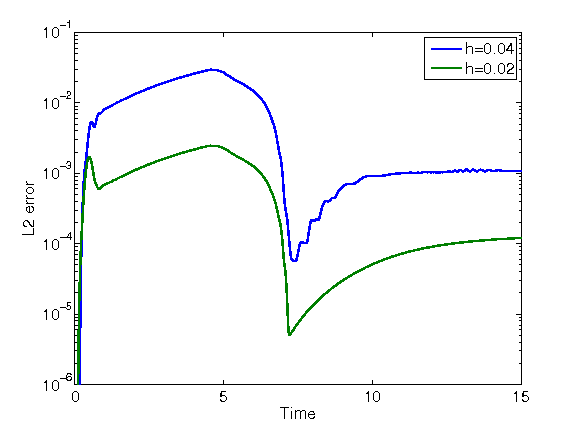
\includegraphics[width=0.7\textwidth]{lamb-err.png}
\caption{The max norm of the error in the solution of Lamb's problem, as function of time. The blue
and green lines correspond to $h=0.04$ and $h=0.02$, respectively.}
\label{fig:lamb-err}
\end{center}
\end{figure}


%% Here we provide input files with four different grid sizes, with $116^2\times 59$, $231^2 \times
%% 116$, $461^2\times 231$, and $921^2\times 461$ grid points, respectively. Be aware that the finest
%% grid uses about 391 Million grid points and can only be run on a sufficiently large machine. The
%% corresponding output files are given in
%% \begin{verbatim}
%% Lambtest1.out  Lambtest2.out  Lambtest3.out  Lambtest4.out
%% \end{verbatim}
%% Note that the most important information is near the end of these files, where the error in the numerical
%% solution is reported. 

\section{Point moment tensor test (not done)}\label{sec:testpointsource}
\index{testing!pointsource}

%%%%%%%%%%%%%%%%%%%%%%%%%%%%%%%%%%%%%%%%%%%%%%%%%%%%%%%%%%%%%%%%%
\chapter{Run time and memory requirements (not done)}\label{sec:performance}
\index{performance}
%%%%%%%%%%%%%%%%%%%%%%%%%%%%%%%%%%%%%%%%%%%%%%%%%%%%%%%%%%%%%%%%%

\section{Run time (not done)}
UPDATE!
%% The execution times shown in Table \ref{tab:cputime-usage} were obtained by running \emph{SW4} on a problem
%% with 5e5 to 1e6 grid points per processor. Timings were measured on 16 processors of the sierra
%% machine at LLNL, in July of 2011. The \emph{SW4} executable was compiled with Intel compilers at
%% optimization level -O. While the absolute numbers in Table \ref{tab:cputime-usage} are machine
%% dependent and destined to change in the (near) future, the relative cost of various solver
%% configurations is likely to stay more or less constant. Note that the visco-elastic cases used 3
%% mechanisms. For the case with topography, about 82\% of the grid points were in the curvilinear
%% grid.

%% We note that 1): solving the visco-elastic wave equations with m=3, requires a factor 3.7 more CPU
%% time than the purely elastic case. 2): Satisfying the interface conditions for grid refinement is
%% relatively expensive. With one refinement and the elastic solver, those conditions required
%% approximately 60\% of the total computation time.  For the visco-elastic case, more calculations per
%% grid point are performed in the interior of the domain, and the relative cost for enforcing the
%% interface conditions goes down to about 35\% of the total time. 3): The strong scaling properties
%% are not perfect. Hence, the performance might be degraded when the number of processors is increased
%% while keeping the number of grid points fixed. More experimentation is needed to better evaluate the strong
%% scaling properties of \emph{SW4}.

%% \begin{table}
%% \begin{center}
%% \begin{tabular}{|l|l|r|r|}\hline
%% Configuration              & Solver        & Execution time [s] & Relative factor \\ \hline\hline
%% Cartesian, single grid     & elastic       & $6.90\cdot 10^{-9}$ & 1 \\ \hline
%% Cartesian, one refinement  & elastic       & $1.64\cdot 10^{-8}$ & 2.4 \\ \hline
%% Cartesian, two refinements & elastic       & $1.77\cdot 10^{-8}$ & 2.7 \\ \hline
%% Topography                 & elastic       & $3.48\cdot 10^{-8}$ & 5.0 \\ \hline
%% %Cartesian, single grid     & visco-elastic & $2.57\cdot 10^{-8}$ & 3.7\\ \hline
%% %Cartesian, one refinement  & visco-elastic & $3.49\cdot 10^{-8}$ & 5.1\\ \hline
%% %Topography                 & visco-elastic & $1.27\cdot 10^{-7}$ & 18.0\\ \hline
%% \end{tabular}
%% \end{center}
%% \caption{Execution time per time step and grid point for different grid configurations, both for
%%   solving the elastic and the visco-elastic wave equations. The relative factor is the execution time
%%   relative to the Cartesian single grid case, for the elastic wave equation.}\label{tab:cputime-usage}
%% \end{table}

\section{Memory usage (not done)}

UPDATE! 
%% The memory usage in Table~\ref{tab:mem-usage} was obtained by running \emph{SW4} on a single processor
%% using 1-2 M grid points. By inspection of the source code, we found the following number of 3-D
%% arrays holding double precision (8 bytes) floating point variables:
%%  15 for Cartesian grids, another
%% 13 for topography (coordinates and metric coefficients in the curvilinear grid), and an additional
%% 5+11*m for a m-mechanism visco-elastic material. These numbers correspond to the asymptotic memory
%% requirements presented in the right column of Table \ref{tab:mem-usage}, which agree well with the
%% observed memory usage. The observed numbers tend to the theoretical asymptotic numbers as the
%% problem size increases.
%% \begin{table}
%% \begin{center}
%% \begin{tabular}{|l|l|r|r|}\hline
%% Configuration   &  solver       & Memory [bytes/grid point]  & Asymp. usage [bytes/grid point] \\ \hline\hline
%% Cartesian grid  & elastic       & 135 & 120 \\ \hline
%% Topography      & elastic       & 228 & 205 \\ \hline 
%% %Cartesian grid  & visco-elastic & 440 & 424 \\ \hline 
%% %Topography      & visco-elastic & 530 & 509 \\ \hline 
%% \end{tabular}
%% \end{center}
%% \caption{Memory usage for different grid and solver configurations. The visco-elastic case has 3
%%   mechanisms and the case with topography has 82\% of the grid point in the curvilinear
%%   grid.}\label{tab:mem-usage}
%% \end{table}

%% As expected, the observed memory usage closely follows the linear relation
%% \[
%%  M=k*N+m, 
%% \]
%% where M is memory usage and N is the number of grid points. For parallel runs, the memory per
%% grid point will be somewhat higher, because of duplicated ghost points at the processor
%% boundaries. Here we only report the memory usage for a single processor run. Note that the
%% volimage command saves a copy of the image variable over the full 3D volume. This adds (at single
%% precision, and full resolution) 4 bytes per grid point and per volume image command. It is possible
%% to reduce this size by only saving every n:th grid point in each coordinate direction. For example,
%% only saving every 2nd point reduces the size of the data by a factor 8.

\printindex

\bibliographystyle{plain}

\bibliography{refs} 


\end{document}
